% -----------------------------------------------------------------
% Vorlage fuer Ausarbeitungen von
% Bachelor- und Masterarbeiten am ISS
% 
% Template for written reports or master theses at the ISS
% 
% For use with compilers pdflatex or latex->dvi2ps->ps2pdf.
%
% -----------------------------------------------------------------
% README, STUDENT USERS:
% We highly appreciate students using this template _AS IS_,period. 
% The document provides adjustable document preferences, 
% student information settings and typography definitions. Look for
% code delimited by *** ***
%
% The short explanation: it's the ISS common standard and 
% 	it's battle tested.
% The long explanation: 
%	We do not want you to go through the document and tweak the 
%	package options, layout parameters and line skips here and 
%	there and waste hours. We are providing this template such 
%	that you can fully concentrate on filling in the much more 
%	important _contents_ of your thesis.
%
% If you have serious needs on extra packages or design 
% modifications, talk to your supervisor _before_ modifying 
% the template.
% Similarly, we're happy if you give your supervisor a hint on any 
% errors in this template.
%
% -----------------------------------------------------------------
% History:
% Jan Scheuing,   04.03.2002
% Markus Buehren, 20.12.2004
% last changes:   10.01.2008 (removed unused packages), 
% 		07.08.2009 (added IEEEtran_LSS.bst file)
% 		02.05.2011 removed matriculation number from cover page
% Martin Kreissig, 25.01.2012: all eps/ps parts removed for 
% 				pdflatex to work properly
% Peter Hermannstaedter, 14.08.2012: fusion of versions for 
% 		latex/dvi/ps/pdf and pdflatex, additional comments,
% 		unification of document flags and student options
% Florian Liebgott, 12.03.2015: bug fixes, removal of obsolete options,
%		switch to UTF-8
% Florian Liebgott, 20.05.2015: fixed encoding problem on title page
% Florian Liebgott, 24.01.2017: changed deprecated font commands (like
%		\sl) to up-to-date commands to be compatible with
%		current TeX distributions.
% Felix Wiewel, 30.08.2021: Replace obsolete scrpage2 with scrlayer-scrpage
%
% -----------------------------------------------------------------
% If you experience any errors caused by this template, please
% contact Florian Liebgott (florian.liebgott@iss.uni-stuttgart.de)
% or your supervisor, so we can fix the errors.
% -----------------------------------------------------------------


\documentclass[12pt,DIV14,BCOR12mm,a4paper,footinclude=false,headinclude,parskip=half-,twoside,openright,cleardoublepage=empty,toc=index,bibliography=totoc,listof=totoc]{scrreprt}
% encoding needs to be defined here, otherwise umlauts on the titelpage won't work.
\usepackage[utf8]{inputenc}
\usepackage{acronym}
\usepackage{setspace}
\usepackage{textgreek}
\usepackage{enumitem}
\usepackage{algorithm}
\usepackage{algorithmic}
% \usepackage{algpseudocode}
\usepackage{graphicx}
\usepackage{subcaption}
\usepackage{adjustbox}
\usepackage{makecell}
\usepackage{amsmath, amssymb, mathrsfs}
\usepackage[abbreviations,symbols,style=index]{glossaries-extra}
\usepackage[acronym]{glossaries}
\usepackage{abstract}
\usepackage[sorting=none]{biblatex}
\addbibresource{refs.bib}%
\usepackage{multirow}
\usepackage{cleveref}
\usepackage{dirtree}
\usepackage{pifont}
\usepackage{float}
\usepackage{makecell}
\usepackage{siunitx}
%
%
% *****************************************************************
% -------------------> document preferences here <-----------------
% *****************************************************************
% Uncomment the settings you like and comment the settings you don't
% like.

% Language: 
% affects generic titles, Figure term, titlepage and bibliography
% (Note:if you switch the language, compile tex and bib >2 times)
\def \doclang{english} 	% For theses/reports in English
%\def \doclang{german} 		% For theses/reports in German

% Hyperref links in the document:
\def \colortype{color} % links with colored text
%\def \colortype{bw} 	% plain links, standard text color (e.g. for print)
%\def \colortype{boxed} % links with colored boxes
% *****************************************************************
%
%
%
% *****************************************************************
% --------------> put student information here <------------------
% *****************************************************************
% Please fill in all items denoted by "to be defined (TBD)"
\def \deworktitle{Upsampling der Range-Doppler-Karte für einkanaliges Chirp-Sequence-Radar unter Verwendung von Deep Learning}        % German title/translation
\def \enworktitle{Range-Doppler map upsampling for single channel chirp sequence radar using Deep Learning}        % English title/translation
\def \tutor{Sven Hinderer}
\def \student{Zheming Yin}
\def \worksubject{Masterarbeit D1513}  % type and number (S/Dxxxx) of your thesis
\def \startdate{01.10.2024}
\def \submission{31.03.2025}
\def \signagedate{31.03.2025}   % Date of signature of declaration on last page
\def \keywords{Range-Doppler map, Image upsampling, Transformer, cGAN, Data collection, Data processing, Loss combination}
%\def \abstract{Abstract TBD}

% *****************************************************************
%

\usepackage{amsmath}
\usepackage{amsfonts}
\usepackage{ifthen}
\ifthenelse{\equal{\doclang}{german}}{
	\usepackage[ngerman]{babel} %german version
	\def \maintitle{\deworktitle}
	\def \translatedtitle{\enworktitle}
	% set , to decimal and . to thousands separator, if German language is used
	\DeclareMathSymbol{,}{\mathord}{letters}{"3B}
	\DeclareMathSymbol{.}{\mathpunct}{letters}{"3A}
	}{
	%english version
	\def \maintitle{\enworktitle}
	\def \translatedtitle{\deworktitle}
	}
\usepackage{txfonts} % Times-Fonts
\usepackage[T1]{fontenc}
\usepackage{color}
\usepackage[headsepline]{scrlayer-scrpage} % Headings

\usepackage{graphicx}
\usepackage[format=hang]{caption}       % for hanging captions
\usepackage{subfig}                     % for subfigures
\usepackage{wrapfig}                    % for figures floating in text, alternatively you can use >>floatflt<<
\usepackage{booktabs}                   % nice looking tables (for tables with ONLY horizontal lines)

%%%%% Tikz / PGF - drawing beautiful graphics and plots in Latex
% \usepackage{tikz}
% \usetikzlibrary{plotmarks}              % larger choice of plot marks
% \usetikzlibrary{arrows}                 % larger choice of arrow heads
% % ... insert other libraries you need
% \usepackage{pgfplots}
% % set , to decimal and . to thousands separator for plots, if German language is used
% \ifthenelse{\equal{\doclang}{german}}{
% \pgfkeys{/pgf/number format/set decimal separator={,}}
% \pgfkeys{/pgf/number format/set thousands separator={.}}
% }{}
%%%%%%

\ifthenelse{\equal{\colortype}{color}}{
	% colored text version:
	\usepackage[colorlinks,linkcolor=blue]{hyperref}
	\newcommand{\bugfix}{\color{white}{\texttt{\symbol{'004}}}} % Bug-Fix Umlaute in Verbatim
}{
	\ifthenelse{\equal{\colortype}{boxed}}{
		% colored box version:
		\usepackage{hyperref}
		\newcommand{\bugfix}{\color{white}{\texttt{\symbol{'004}}}} % Bug-Fix Umlaute in Verbatim
	}{
		% monochrome version:
		\usepackage[hidelinks]{hyperref}
		\newcommand{\bugfix}{\color{white}{\texttt{\symbol{'004}}}} % Bug-Fix Umlaute in Verbatim
	}
}

% Layout and Headings
\pagestyle{scrheadings}
\automark{chapter}
\clearscrheadfoot
\lehead[]{\pagemark~~\headmark}
\rohead[]{\headmark~~\pagemark}
\renewcommand{\chaptermark}[1]{\markboth {\normalfont\slshape \hspace{8mm}#1}{}}
\renewcommand{\sectionmark}[1]{\markright{\normalfont\slshape \thesection~#1\hspace{8mm}}}
\addtolength{\textheight}{15mm}
\parindent0ex
\setlength{\parskip}{5pt plus 2pt minus 1pt}
\renewcommand*{\pnumfont}{\normalfont\slshape} % Seitenzahl geneigt
\renewcommand*{\sectfont}{\bfseries} % Kapitelueberschrift nicht Helvetica

% Settings for PDF document
\pdfstringdef \studentPDF {\student} 
\pdfstringdef \worktitlePDF {\maintitle}
\pdfstringdef \worksubjectPDF {\worksubject}
\hypersetup{pdfauthor=\studentPDF, 
            pdftitle=\worktitlePDF,
            pdfsubject=\worksubjectPDF}

% Title page
\titlehead{
	
\includegraphics[width=20mm]{university-logo}
	\hspace{6mm}
	\ifthenelse{\equal{\doclang}{german}}{
		\begin{minipage}[b]{.6\textwidth}
		{\Large Universit\"at Stuttgart } \\
		Institut f\"ur Signalverarbeitung und Systemtheorie\\
		Professor Dr.-Ing. B. Yang \vspace{0pt}
		\end{minipage}
	}{
		\begin{minipage}[b]{.6\textwidth}
		{\Large University of Stuttgart } \\
		Institute for Signal Processing and System Theory\\
		Professor Dr.-Ing. B. Yang \vspace{0pt}
		\end{minipage}
	}
	\hspace{1mm}
	
\includegraphics[width=28mm]{isslogocolor}
}
\subject{\worksubject\vspace*{-5mm}} % Art und Nummer der Arbeit
\title{\maintitle}%\\ \Large{\subtitle}}
\subtitle{\translatedtitle}
\author{
\large
  \ifthenelse{\equal{\doclang}{german}}{
  \begin{tabular}{rp{7cm}}
    \Large 
    Autor:      & \Large \student \vspace*{2mm}\\
    Ausgabe:    & \startdate \\
    Abgabe:     & \submission \vspace*{3mm}\\
    Betreuer:   & \tutor \vspace*{2mm}\\
    Stichworte: & \keywords
  \end{tabular}
  }{
  \begin{tabular}{rp{7cm}}
    \Large 
    Author:             & \Large \student \vspace*{2mm}\\
    Date of work begin: & \startdate \\
    Date of submission: & \submission \vspace*{3mm}\\
    Supervisor:         & \tutor \vspace*{2mm}\\
    Keywords:           & \keywords
  \end{tabular}
  }
  \bugfix
}
\date{}
\publishers{\normalsize
  \begin{minipage}[t]{.9\textwidth}
    \abstract
  \end{minipage}
}

\numberwithin{equation}{chapter} 
\sloppy 

%
%
%
% *****************************************************************
% --------------> put typography definitions here <----------------
% *****************************************************************
% colors
\definecolor{darkblue}{rgb}{0,0,0.4}

% declarations
\newcommand{\matlab}{\textsc{Matlab}\raisebox{1ex}{\tiny{\textregistered}} }
% Integers, natural, real and complex numbers
\newcommand{\Z}{\mathbb{Z}}
\newcommand{\N}{\mathbb{N}}
\newcommand{\R}{\mathbb{R}}
\newcommand{\C}{\mathbb{C}}
% expectation operator
\newcommand{\E}{\operatorname{E}}
% imaginary unit
\newcommand{\im}{\operatorname{j}}
% Euler's number with exponent as parameter, e.g. \e{\im\omega}
\newcommand{\e}[1]{\operatorname{e}^{\,#1}}
% short command for \operatorname{}
\newcommand{\op}[1]{\operatorname{#1}}

% unknown hyphenation rules
\hyphenation{Im-puls-ant-wort Im-puls-ant-wort-ko-ef-fi-zien-ten
Pro-gramm-aus-schnitt Mi-kro-fon-sig-nal}
% *****************************************************************
%

\makeglossaries

\newabbreviation{adagrad}{Adagrad}{Adaptive gradient algorithm}
\newabbreviation{adam}{Adam}{Adaptive Moment Estimation}
\newabbreviation{adc}{ADC}{Analog-to-Digital Converter}
\newabbreviation{api}{API}{Application Program Interface}

\newabbreviation{bgd}{BGD}{Batch Gradient Descent}

\newabbreviation{cfar}{CFAR}{Constant False Alarm Rate}
\newabbreviation{cgan}{cGAN}{Conditional Generative Adversarial Networks}
\newabbreviation{cmgan}{CMGAN}{Conformer-Based Metric-GAN}
\newabbreviation{cnn}{CNN}{Convolutional Neural Network}
\newabbreviation{cpi}{CPI}{Coherent Processing Interval}
\newabbreviation{cri}{CRI}{Chirp Repetition Interval}

\newabbreviation{dc}{DC}{Direct Current}
\newabbreviation{dft}{DFT}{Discrete Fourier Transform}
\newabbreviation{dp}{DP}{Dual-Path}

\newabbreviation{fft}{FFT}{Fast Fourier Transform}
\newabbreviation{ffw}{FFW}{Feed-Forward}
\newabbreviation{fm}{FM}{Frequency Modulated}
\newabbreviation{fmcw}{FMCW}{Frequency Modulated Continuous Wave}
\newabbreviation{fol}{FOL}{Frame Of Length}

\newabbreviation{gan}{GAN}{Generative Adversarial Networks}
\newabbreviation{gpu}{GPU}{Graphics Processing Unit}

\newabbreviation{hq}{HQ}{High-Quality}

\newabbreviation{if}{IF}{Intermediate Frequency}
\newabbreviation{ifft}{iFFT}{Inverse Fast Fourier Transform}
\newabbreviation{irdp}{iRDP}{Inverse Range-Doppler Processing}
\newabbreviation{irfft}{irFFT}{Inverse Real-valued Fast Fourier Transform}
\newabbreviation{iss}{ISS}{Institut f\"ur Signalverarbeitung und Systemtheorie}
\newabbreviation{i/o}{I/O}{Input/Output}

\newabbreviation{ln}{LN}{Layer Normalization}
\newabbreviation{lsd}{LSD}{Logarithmic Spectral Distance}
\newabbreviation{lq}{LQ}{Low-Quality}

\newabbreviation{mlp}{MLP}{Multi-Layer Perceptron}
\newabbreviation{mimo}{MIMO}{Multiple input, multiple output}
\newabbreviation{msa}{MSA}{Multi-head Self-Attention}
\newabbreviation{mse}{MSE}{Mean Square Error}

\newabbreviation{plsd}{PLSD}{Phase-aware Logarithmic Spectral Distance}
\newabbreviation{pmse}{PMSE}{Pixel-wise Mean Squared Error}
\newabbreviation{psnr}{PSNR}{Peak Signal-Noise Ratio}

\newabbreviation{ra}{RA}{Range-Azimuth}
\newabbreviation{rdp}{RDP}{Range-Doppler Processing}
\newabbreviation{relu}{ReLU}{Rectified Linear Unit}
\newabbreviation{rfft}{rFFT}{Real-valued Fast Fourier Transform}
\newabbreviation{rmsprop}{RMSProp}{Root Mean Square Prop}
\newabbreviation{rnn}{RNN}{Recurrent Neural Networks}
\newabbreviation{rstb}{RSTB}{Residual Swin Transformer Blocks}
\newabbreviation{rx}{Rx}{Receiver}

\newabbreviation{sar}{SAR}{Synthetic Aperture Radar}
\newabbreviation{sdr}{SDR}{Signal-to-Distortion Ratio}
\newabbreviation{sdk}{SDK}{Software Development Kit}
\newabbreviation{sd-sdr}{SD-SDR}{Scale-Dependent Signal-to-Distortion Ratio}
\newabbreviation{sgd}{SGD}{Stochastic Gradient Descent}
\newabbreviation{si-sdr}{SI-SDR}{Scale-Independent Signal-to-Distortion Ratio}
\newabbreviation{snr}{SNR}{Signal-to-Noise Ratio}
\newabbreviation{stft}{STFT}{Short-Time Fourier Transform}
\newabbreviation{stl}{STL}{Swin Transformer Layers}
\newabbreviation{swin}{Swin}{Shifted Windows}
\newabbreviation{swinir}{SwinIR}{Image Restoration using Swin Transformer}

\newabbreviation{te}{TE}{Transformer Encoder}
\newabbreviation{tf}{TF}{Time-Frequency}
\newabbreviation{tfrecord}{TFRecord}{TensorFlow Records}
\newabbreviation{tx}{Tx}{Transmitter}

\newabbreviation{vgg}{VGG}{Very Deep Convolutional Networks}

\newabbreviation{wandb}{WandB}{Weights and Biases}
\newabbreviation{wmse}{WMSE}{Weighted MSE}


\begin{document}

% title and table of contents
\pagenumbering{alph}
\maketitle
 \cleardoublepage
\pagenumbering{roman} % roman numbering for table of contents
\tableofcontents
 \cleardoublepage


% Input the abbreviation
\renewcommand{\glossarypreamble}{\glsfindwidesttoplevelname[\currentglossary]}
\setglossarystyle{alttree}
\printunsrtglossary[type=abbreviations]
\cleardoublepage
\noindent

% Input the abstract
\begin{minipage}[t]{\textwidth}
    \chapter*{Abstract}
    \addcontentsline{toc}{chapter}{Abstract}
During the extensive usage of chirp sequence radar, it is often affected by the cost, system limit or regulations, resulting in limited resolution of the range-Doppler map. Meanwhile, the range-Doppler map collected in the indoor environment also puts higher requirements on the model in terms of complexity and high amplitude fluctuation, whereas the current upsampling approaches cannot meet this requirement well. Therefore, this thesis will combine the current upsampling models in the state of the art, such as Transformer and cGAN models, with a series of data processing methods, such as logarithm and normalization operations, and the combination of multiple loss functions to improve the quality of the super-resolution range-Doppler map. In addition, the environmental conditions and data in the public datasets about the range-Doppler map are currently simple, so the dataset of this thesis is collected in the indoor environment by ourselves. In the evaluation phase, we obtain an optimized combination of model, processing methods and loss functions and tune the hyperparameters of the model, which significantly improves the result compared to the other image upsampling approaches.
\end{minipage}%
\hfill
\begin{minipage}[t]{\textwidth}
    \chapter*{Kurzfassung}
    % \addcontentsline{toc}{chapter}{Kurzfassung}
Bei der umfangreichen Nutzung von Chirp-Sequence-Radar ist es häufig von den Kosten, Systembeschränkungen oder Vorschriften beeinflusst, was zu einer limitierten Auflösung der Range-Doppler-Karte führt. Gleichzeitig stellt die in Innenräumen erfasste Range-Doppler-Karte höhere Anforderungen an das Modell hinsichtlich Komplexität und hoher Amplitudenfluktuation, denen aktuelle Upsampling-Methoden nicht gut gerecht werden können. Daher kombiniert diese Masterarbeit aktuelle fortgeschrittene Upsampling-Modelle, wie Transformer- und cGAN-Modelle, mit einer Reihe von Datenverarbeitungsmethoden wie Logarithmierung und Normalisierung sowie die Kombination mehrerer Verlustfunktionen, um die Qualit\"at der hochauflösenden Range-Doppler-Karte zu verbessern. Da die Umgebungsbedingungen und Daten in öffentlichen Datens\"atzen zur Range-Doppler-Karte derzeit noch einfach sind, wurde der Datensatz dieser Arbeit selbst in Innenräumen erfasst. In der Evaluierungsphase erzielen wir eine optimierte Kombination aus Modell, Verarbeitungsmethoden und Verlustfunktionen und optimieren die Hyperparameter des Modells, was das Ergebnis im Vergleich zu anderen Bild-Upsampling-Methoden deutlich verbessert.
\end{minipage}

\cleardoublepage

\setcounter{page}{1}
\pagenumbering{arabic} % arabic numbering for rest of document

% *****************************************************************
% -------------------> start writing here <------------------------

%\chapter{Introduction}
%\section{Explanations}
%As shown in \cite{C2}, we present an equation
%\begin{align}
%	H(\omega) = \int h(t) \e{\im\omega t} \delta t \in \N
%\end{align}
%
%Then we include a graphic in figure \ref{mind} and information about captions in table \ref{captions}.\\
%\begin{figure}
%	\centering
%	
\includegraphics[scale=.3]{isslogocolor}
%	\caption{A beautiful mind}
%	\label{mind}
%\end{figure}
%
%\begin{table}
%    \centering
%    \caption{Where to put the caption}
%    \label{captions}
%    \begin{tabular}{lcc}
%        \toprule
%         & above & below\\
%        \midrule
%        for figures & no & yes\\
%        for tables & yes & no\\
%        \bottomrule
%    \end{tabular}
%\end{table}
%
%
%Lorem ipsum dolor sit amet, consetetur sadipscing elitr, sed diam nonumy eirmod tempor invidunt ut labore et dolore magna aliquyam erat, sed diam voluptua. At vero eos et accusam et justo duo dolores et ea rebum. Stet clita kasd gubergren, no sea takimata sanctus est Lorem ipsum dolor sit amet. Lorem ipsum dolor sit amet, consetetur sadipscing elitr, sed diam nonumy eirmod tempor invidunt ut labore et dolore magna aliquyam erat, sed diam voluptua. At vero eos et accusam et justo duo dolores et ea rebum. Stet clita kasd gubergren, no sea takimata sanctus est Lorem ipsum dolor sit amet.
%\newpage
%Lorem ipsum dolor sit amet, consetetur sadipscing elitr, sed diam nonumy eirmod tempor invidunt ut labore et dolore magna aliquyam erat, sed diam voluptua. At vero eos et accusam et justo duo dolores et ea rebum. Stet clita kasd gubergren, no sea takimata sanctus est Lorem ipsum dolor sit amet. Lorem ipsum dolor sit amet, consetetur sadipscing elitr, sed diam nonumy eirmod tempor invidunt ut labore et dolore magna aliquyam erat, sed diam voluptua. At vero eos et accusam et justo duo dolores et ea rebum. Stet clita kasd gubergren, no sea takimata sanctus est Lorem ipsum dolor sit amet.

\chapter{Introduction} \label{introduction}
This chapter introduces the chirp sequence radar and the meaning of the range-Doppler map. The motivation and structure of this thesis are subsequent and the state-of-the-art models are explained in this chapter as well.

\section{Chirp sequence radar} \label{chirp sequence radar}
%Introduce the \gls{fmcw}. Introduce the definition of the range-doppler map, how does it look like, how can range and Doppler effect be calculated.
Chirp sequence radar is used in the radar system based on \gls{fmcw} technology, widely used in the field of automotive driving, target detection, and environmental sensing and so on \cite{7556357}. Chirp sequence radar transmits multiple consecutive chirp signals, receives the echoes, and calculates target information such as range and velocity, which can be used to generate a range-Doppler map.

\begin{spacing}{1.5}
\textbf{\large{FMCW radar}}
\end{spacing}

In \gls{fmcw} radar, the chirp frequency increases linearly with time, of which the signal is called the linear \gls{fm} signal. Figure \ref{FMCW_signal} illustrates the change of a linear \gls{fm} chirp in amplitude and frequency over time. The signal frequency will increase from the initial value $f_c$ by the bandwidth $B$ during the duration of one chirp $T_c$. After a time interval, the other chirp will be transmitted at time $T_p$. The rate of the frequency change is shown as the slope, namely $S=B/T_c$.

With this property, we can get the range and velocity of the other targets related to the \gls{fmcw} radar. There will be a delay between the signal being transmitted and being received by the radar, which is proportional to the range. Since the signal is a round trip motion, the range between the radar and the target can be defined as

\begin{equation}
    \centering
    r = c \cdot \frac{\tau}{2},
    \label{propagation delay formula}
\end{equation}

where $c$ represents the speed of light, namely $3 \times 10^8$ m/s, and $\tau$ represents the propagation delay. The Doppler effect refers to the phenomenon that the frequency of the received signal and the transmitted signal will be different when there is a relative velocity between the signal source and the target. The relationship between the frequency of the transmitted signal $f$ and the received signal $f'$ is

\begin{equation}
    \centering
    f' = f \left( \frac{c \pm v_o}{c \mp v_s} \right),
    \label{doppler shift formula}
\end{equation}

where $v_0$ and $v_s$ represent the relative velocity of the radar and target. When they move towards each other, the frequency of the received signal increases, and vice versa. In the collected dataset, the radar as the signal source is moving, while the surrounding objects are stationary in most cases.

\begin{figure}
    \centering
    \hspace{-0.4cm}
    \begin{subfigure}{0.45\textwidth}
        \centering
        \adjustbox{height=5cm}{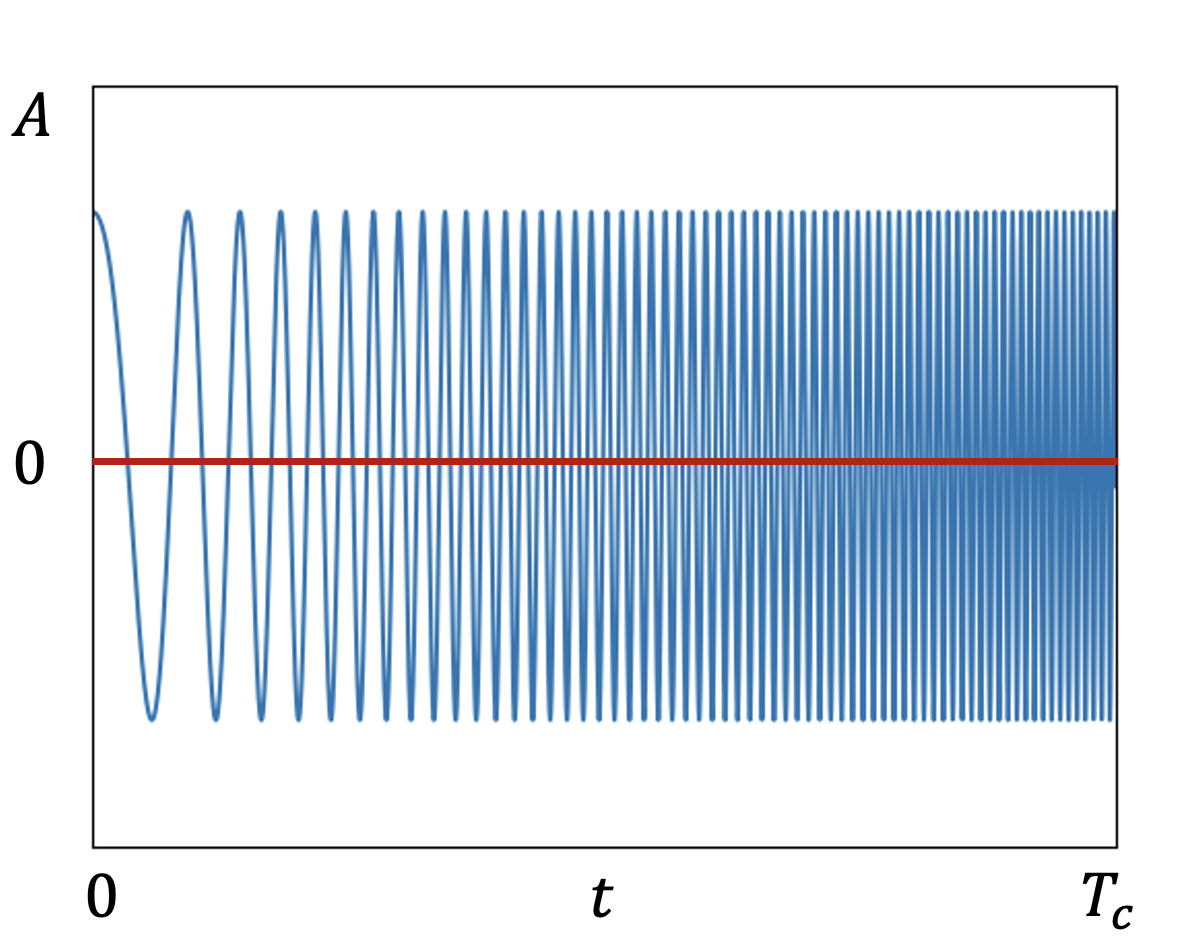
\includegraphics[scale=.3]{figures/FMCW_signal_left.png}}
    \end{subfigure}
    \begin{subfigure}{0.45\textwidth}
        \centering
        \adjustbox{height=5cm}{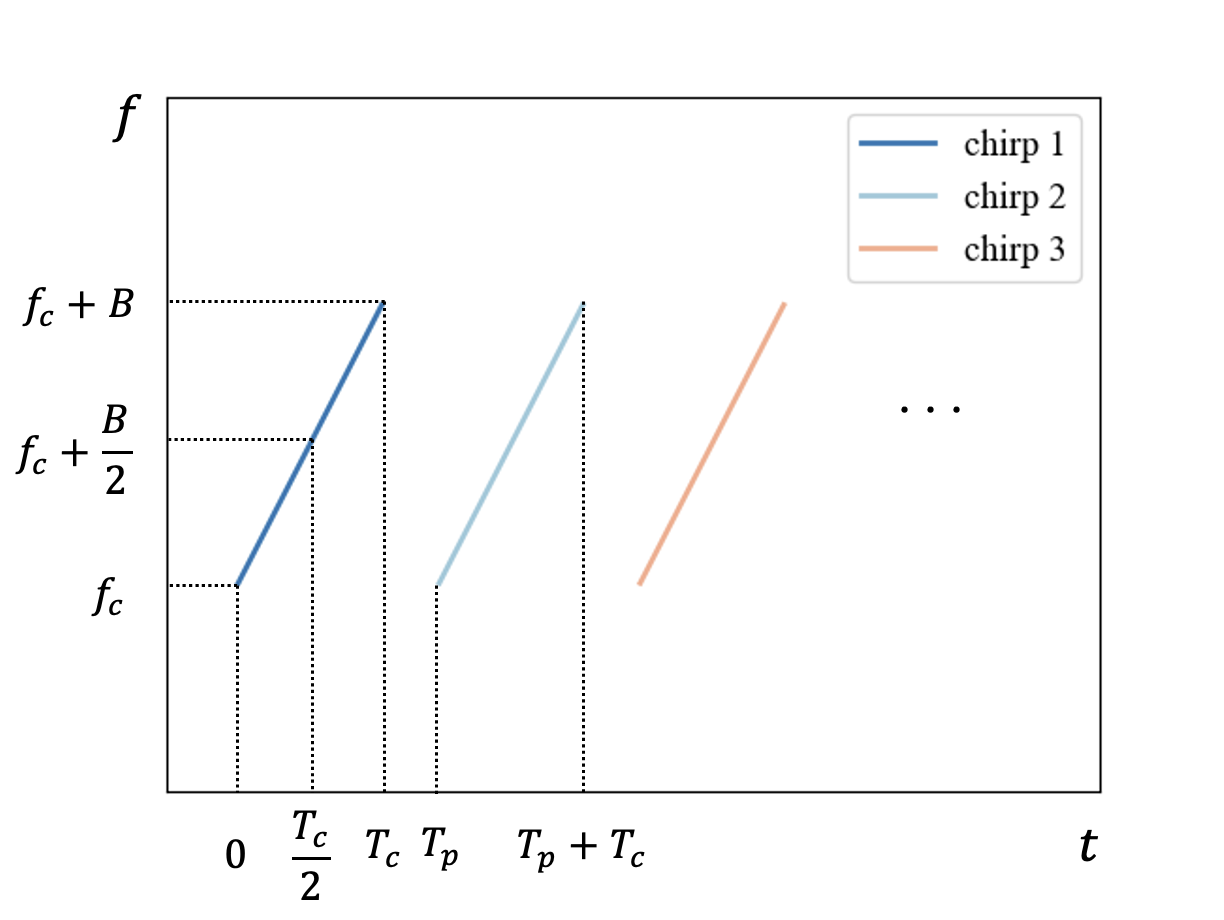
\includegraphics[scale=.3]{figures/FMCW_signal_right.png}}
    \end{subfigure}
    \caption{The amplitude and frequency variation of FMCW radar in time respectively.}
	\label{FMCW_signal}
\end{figure}

Meanwhile, as the reflected signal is captured by the radar, it will be mixed with the transmitted signal in the system to obtain a new signal called \gls{if} signal. The frequency of this \gls{if} signal is theoretically not only depending on the frequency shift $f_r$ caused by the propagation distance but also the Doppler frequency $f_d$, according to \cite{7556357} written as

\begin{equation}
    \centering
    f\textsubscript{IF}\ = f_r - f_d = S \cdot \frac{2r}{c} - \frac{2v}{\lambda},
\end{equation}

but in our case, the Doppler frequency $f_d$ in the beat frequency can be ignored due to the property of the chirp sequence radar, namely

\begin{equation}
    \centering
    f\textsubscript{IF}\ = f_r = S \cdot \frac{2r}{c},
\end{equation}

where the reason will be shown in the next explanation of the chirp sequence radar.

\begin{spacing}{1.5}
\textbf{\large{Chirp sequence radar}}
\end{spacing}

The chirp sequence radar is a \gls{fmcw} radar with the steep frequency ramps \cite{fink_comparison_2015}. The dataset in this paper are collected by a single channel chirp sequence radar \cite{ag_bgt60tr13c_nodate}, which means only a single transmitter and a single receiver are used. In section \ref{dataset recording}, the hardware of the chirp sequence radar will be explained in detail, where there are a single transmitter and three receivers in the radar device. The advantages of using the single channel are following, on one hand, the \gls{mimo} radar will cause a higher cost, hence the single channel radar system reduce the cost to make the localization system cheaper. On the other hand, the signal needs to do the \gls{fft} to convert the signal from time domain into the frequency domain, and the computational complexity will be decreased accordingly.

Due to the difference in the rate of frequency change, the advantage of chirp sequence radar is removing the Doppler frequency part from the \gls{if} signal as mentioned above. The reason is that with the short chirp, i.e. the high value of the slope $S$, the frequency shift $f_r$ will be much larger than the Doppler frequency $f_d$ part. With this property, the radar system will be easy to de-couple the range and velocity estimation, where the range can be calculated by the \gls{if} signal frequency. The estimation of the range is within each chirp which is called the fast time axis, whereas the velocity is calculated by the frequencies of the transmitted and received signals according to the Doppler shift between the chirps which is called the slow time axis, since the time interval between the samples within the chirp is quite short.

\begin{spacing}{1.5}
\textbf{\large{Range-Doppler map}}
\end{spacing}

According to the above, the chirp sequence radar based on the \gls{fmcw} radar can also obtain information about the range and velocity. Meanwhile, there is a corresponding relationship between the range and velocity, which can be drawn through the range-Doppler map. The derivation and visualization process will be shown in detail in section \ref{range-Doppler map visualization}, where the range-Doppler map looks like the one in Figure \ref{an example of the range-Doppler map}.

\begin{figure}
	\centering
	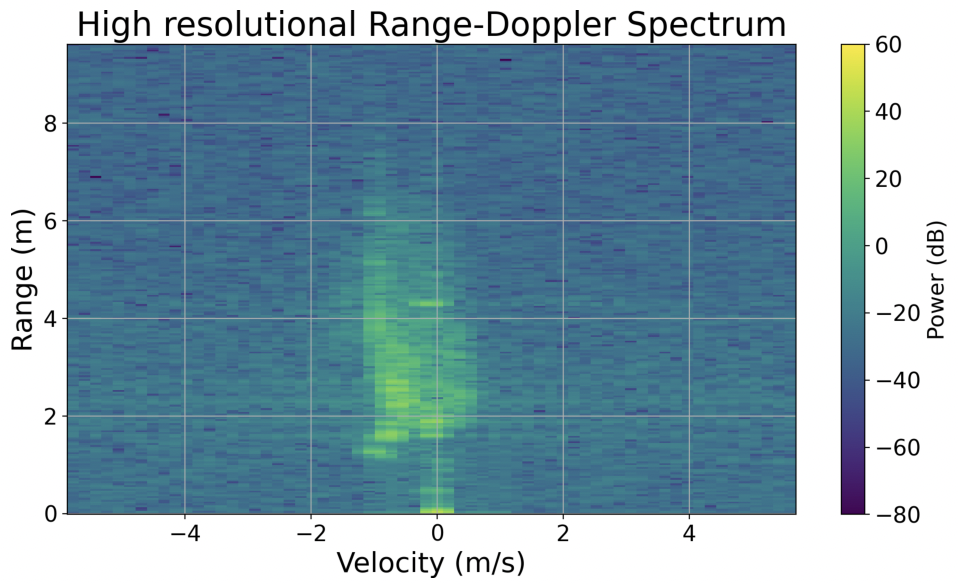
\includegraphics[scale=.6]{thesis/figures/high_res_new.png}
	\caption{An example of the range-Doppler map.}
	\label{an example of the range-Doppler map}
\end{figure}

In the range-Doppler map, the horizontal and vertical axes denote velocity and range respectively. In our dataset, the range is calculated from 0 m to roughly 10 m, and the velocity changes from roughly -5 m/s to 5 m/s. At each point where the range and velocity intersect, the value represents the amplitude about the signal power. When the amplitude is converted to dB unit, the value range is between -80 dB and 60 dB, and the corresponding color in the bar gradually changes from dark to light.


\section{Motivation} \label{motivation}
%The motivation of this thesis and structure of the thesis, show how does the data look like.
As mentioned above, the chirp sequence radar can achieve a larger bandwidth and higher range resolution, but in practical applications, many factors will limit the resolution, such as the hardware of the radar and \gls{cpi}. The carrier frequency and the bandwidth are fixed values in a radar system, since the large bandwidth or high frequency put a higher requirements on the hardware, such as \gls{adc}, antennas and so on, if the cost of the radar system is limited, that is, the frequency or bandwidth are limited, both range and velocity resolutions are influenced. The carrier frequency used by the radar system is affected by many other factors as well, such as regulation. \gls{cpi} refers to the time interval in which the radar continuously observes the targets and performs signal processing. The signal during this time period is coherent, that is, the phase of the signal remains stable and does not change significantly. \gls{cpi} is inversely proportional to the Doppler frequency resolution. In this process, the longer the \gls{cpi}, the more accurate the Doppler frequency resolution can be obtained which leads to a more accurate velocity estimation. However, in many cases, due to the movement of the targets or the ego-motion of the radar itself, the \gls{cpi} is limited, which in turn affects the velocity resolution.

When Figure \ref{an example of the range-Doppler map} is regarded as a high-resolution range-Doppler map, then in reality, the resolution of range and velocity may be only half or even a quarter of that, resulting in a lot of information loss, as shown in Figures \ref{examples of the low resolutional range-Doppler map in different downsampled factor}, where Figure \ref{in halved resolution} shows the effect of the range-Doppler map with the halved resolution, whereas Figure \ref{in quarter resolution} shows a quarter resolutional range-Doppler map.

\begin{figure}
    \centering
    \hspace{-0.4cm}
    \begin{subfigure}{0.5\textwidth}
        \centering
        \adjustbox{height=5cm}{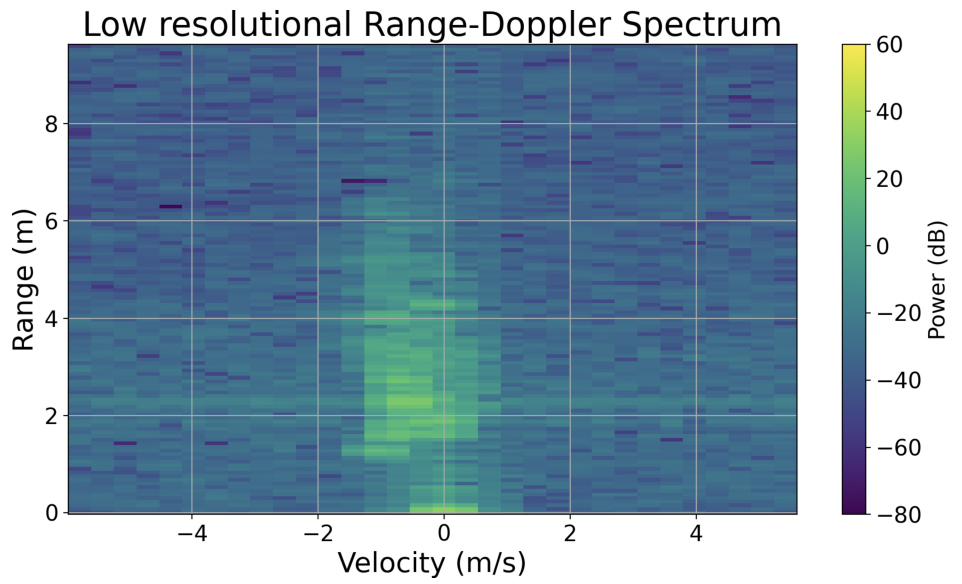
\includegraphics[scale=.24]{thesis/figures/factor_2_new.png}}
        \caption{In halved resolution}
        \label{in halved resolution}
    \end{subfigure}
    \begin{subfigure}{0.5\textwidth}
        \centering
        \adjustbox{height=5cm}{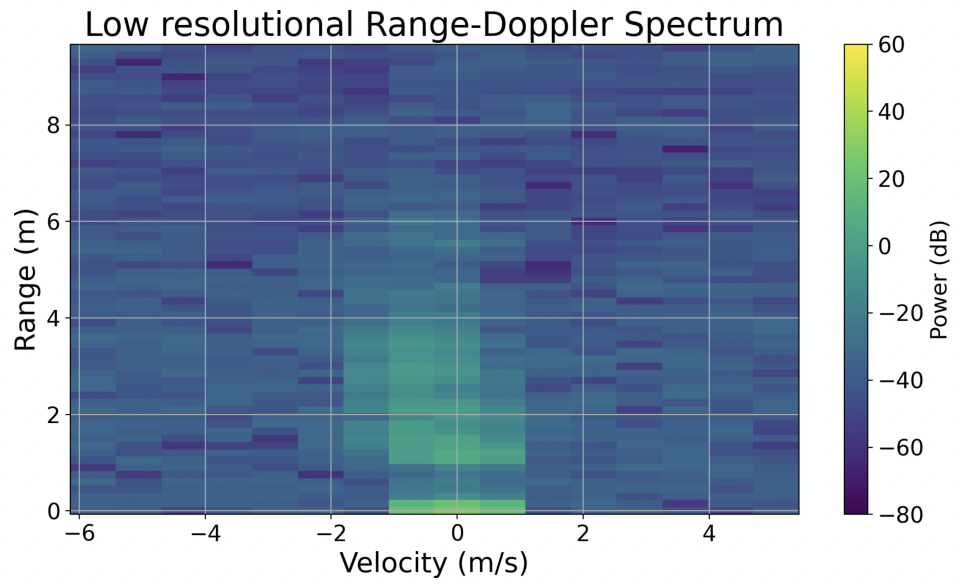
\includegraphics[scale=.24]{thesis/figures/factor_4_new.png}}
        \caption{In quarter resolution}
        \label{in quarter resolution}
    \end{subfigure}
    \caption{Examples of the low-resolution range-Doppler map with different downsampling factor related to the high-resolution range-Doppler map in Figure \ref{an example of the range-Doppler map}.}
	\label{examples of the low resolutional range-Doppler map in different downsampled factor}
\end{figure}

However, high-resolution range-Doppler maps are crucial and have a wide range of applications in areas such as the indoor localization. In order to accurately process and utilize the range-Doppler map, such as \gls{cfar} detection, a high-resolution range-Doppler map is wanted. A traditional, simple and parameter-free method for upsampling is (bi-)linear interpolation. With the development of deep learning, it has shown a strong capability to upsample data to the high resolution. The common structures and models include \gls{cnn}, Encoder-Decoder architecture, Transformer, \gls{cgan} and so on \cite{wang_deep_2021}. Meanwhile, there are also multiple commercial super-resolution solution, such as the super-resolution system in video games provided by NVIDIA \cite{watson2020deep}.

However, the current upsampling approaches are mainly based on images or videos generally, and rarely specifically based on the range-Doppler map of the indoor environment. Compared with the daily images, the range-Doppler map has several significant characteristics. One is that the data in the range-Doppler map have relatively wide dynamic range, especially in the complex environment such as the indoor environment. According to Figure \ref{an example of the range-Doppler map}, the amplitude can be as high as \SI{40}{dB} in places with a closer range, while the noise will be lower than \SI{-60}{dB} in places farther away from the radar. Furthermore, the values in the range-Doppler map are not as visually coherent as those images in the daily life. In addition to the higher values in the parts with closer range, there are usually large differences between even two adjacent points in the surrounding area, which asks for the special requirements on data processing and structure of the model. We would like to process the data so that its dynamic range is relatively smaller. Meanwhile, since each point in the range-Doppler map contains a variety of information such as velocity, range and power, there is a certain correlation between these informations. We hope that the model can learn the connection and relationship between different areas and use deep learning to achieve better upsampling effect than the traditional methods, such as interpolation, and the models commonly used in computer vision.

In addition, another challenge is that our goal is not just based on the closer part, i.e., the area with higher amplitude, but the entire range-Doppler map, including the signals with the lower amplitude. Therefore, in data processing, the purpose of making the range of amplitude smaller not only reduces the dynamic range of the data, but also allows the lower amplitude signals to receive attention.

This thesis will mainly focus on three parts: dataset, models, and loss functions. We will use the radar in the \gls{iss} at the University of Stuttgart to collect the data of the range-Doppler maps and process the dataset. The pipeline will be built to load and process dataset, build and train models, and evaluate them. We will also choose the best data processing methods and the combination of loss functions as well to achieve better upsampling effects for range-Doppler maps.

\section{Structure of the thesis} \label{structure of the thesis}
The thesis will consist of seven chapters. Chapter \ref{introduction} focuses on the introduction of the content in the title and the explanation of some basic concepts, which are completed in section \ref{chirp sequence radar}. Section \ref{motivation} introduced the motivation of the upsampling task based on the range-Doppler map, the challenges, and the ultimate goal of this thesis. Section \ref{structure of the thesis} shows the main structure of the entire thesis and each section. Section \ref{overview of the state of the art} shows the current upsampling approaches in the state of the art, including but not limited to upsampling models for range-Doppler maps.

Chapter \ref{dataset} will focus on the data part. Section \ref{dataset recording} will introduce the information about the data collection, including the hardware of the radar used, the parameters of radar initialization, the settings during the collection process, such as the motion and environmental conditions, and the size of the collected dataset. Moreover, in order to meet our needs, the parameters of the radar as well as the resolution equations will be derived and calculated during the initialization. Section \ref{dataset loading} will show the process of dataset loading, using \gls{tfrecord} files to store data and speed up the loading and training process, and the setting of parameters while creating \gls{tfrecord} files, such as the number of frames, where we use a sliding window for that and the augmentation. In addition, the resampling operation of the data will be demonstrated. Based on the collected high-resolution data, i.e., the ground truth, we create paired low-resolution and high-resolution tuples for training and evaluation by downsampling the high-resolution signals to their respective low-resolution representation. Meanwhile, since the visualization of the range-Doppler map is in the frequency domain, the conversion between the time domain and the frequency domain for the range-Doppler map will also be demonstrated. Section \ref{pre- and post-processing of the model inputs and outputs} will show the processing methods on the models' inputs and outputs. Since the model can only deal with the real value rather than complex value, it could be converted into the concatenation of the real and imaginary part or of the amplitude and phase part, and they can be also normalized or applied logarithm operation to reduce the dynamic range.

Chapter \ref{models} is mainly about the deep learning models used, including a basic \gls{cnn} model, a classical UNet structure and a UNet model that concatenates the decoder part with the encoder part, and two different architectures using Transformer, called \gls{dp}-\gls{tf} Transformer model and \gls{swinir} architecture, respectively in section \ref{dp-tf transformer architecture} and \ref{swinir transformer architecture}. The Transformer architectures have also two types, \gls{dp}-\gls{tf} Transformer block and \gls{swin} Transformer block. Section \ref{comparison between the architecture} will compare the differences between the Transformer architectures and blocks. Section \ref{cgan architecture} will use the above models to design a \gls{cgan} model which contains a generator and introduces a discriminator to implement the adversarial model. Furthermore, in the process of converting data from the time domain to the frequency domain, the range dimension will turn to an odd value, such as from 512 to 257, which will cause problems when the model divide the data into the patches or do the downsampling. Therefore, section \ref{dimension processing layer} will focus on this problem and propose two methods. Additionally, the model must undergo an upsampling layer before the output. There are currently two main methods, which will be introduced in section \ref{upsampling layer}.

Chapter \ref{loss functions} focuses on various loss functions in both training and evaluation phases, and based on the effects of different loss functions, section \ref{combination of the losses} will combine them to complement each other. Chapter \ref{training optimization} will show some methods used in the pipeline to optimize the entire training process, such as using multiple GPUs for distributed training to speed up the training process in section \ref{distributed training}, some settings in the pipeline in section \ref{settings in the pipeline}, and the hyperparameters which can be tuned by the sweep function of the tool WandB shown in section \ref{hyperparameter optimization}.

Finally, Chapter \ref{results} shows the impact of multiple settings, such as different models, processing methods as well as loss functions, on the evaluation loss results, the effect of the super-resolution range-Doppler maps and analyzes them. Chapter \ref{summary and outlook} summarizes the results of the entire thesis and gives the outlook on the further research.

\section{Overview of the state of the art} \label{overview of the state of the art}

%The approaches in the reference papers, and introduce some architectures such as Encoder-Decoder, Transformer and Swin Transformer as well as \gls{cgan} which are normally used in image upsampling.

The state-of-the-art super-resolution methods mainly focus on the supervised learning algorithms \cite{wang_deep_2021}. Currently, the models and structures used in the super-resolution field mainly include \gls{cnn}, residual-based methods, encoder-decoder structure, GAN model, etc \cite{wang_deep_2021}. In addition, Transformer has a strong ability in terms of translation task and wording understanding. The model uses Attention mechanism to understand the association and relationship between different words and phrases, so that it can understand longer sentences than \gls{rnn} \cite{vaswani_attention_2023}. Taking advantage of this feature, the \gls{swin} Transfomer designs a shifted window based on Transformer to divide the data patches and shift windows between them, then different windows can also learn the relationship between each other \cite{liu_swin_2021}.

\begin{spacing}{1.5}
\textbf{\large{Encoder-decoder structure}}
\end{spacing}

The encoder-decoder structure includes two parts. First, it will use encoder to extract features, learn the extracted features, and then use the decoder part to restore the input based on those learned features, so that the model can get the required output. A common structure is called UNet. Olaf et al. apply UNet to segment medical images \cite{ronneberger_u-net_2015}. According to Figure \ref{unet architecture}, the structure of their model is U-shaped. The left side of "U" is the encoder part, that is, the features of the data are extracted and learned, and the right side is the part of the decoder which uses the learned features to restore the data back the original size, while segmenting the objects in the image.

\begin{figure}
	\centering
	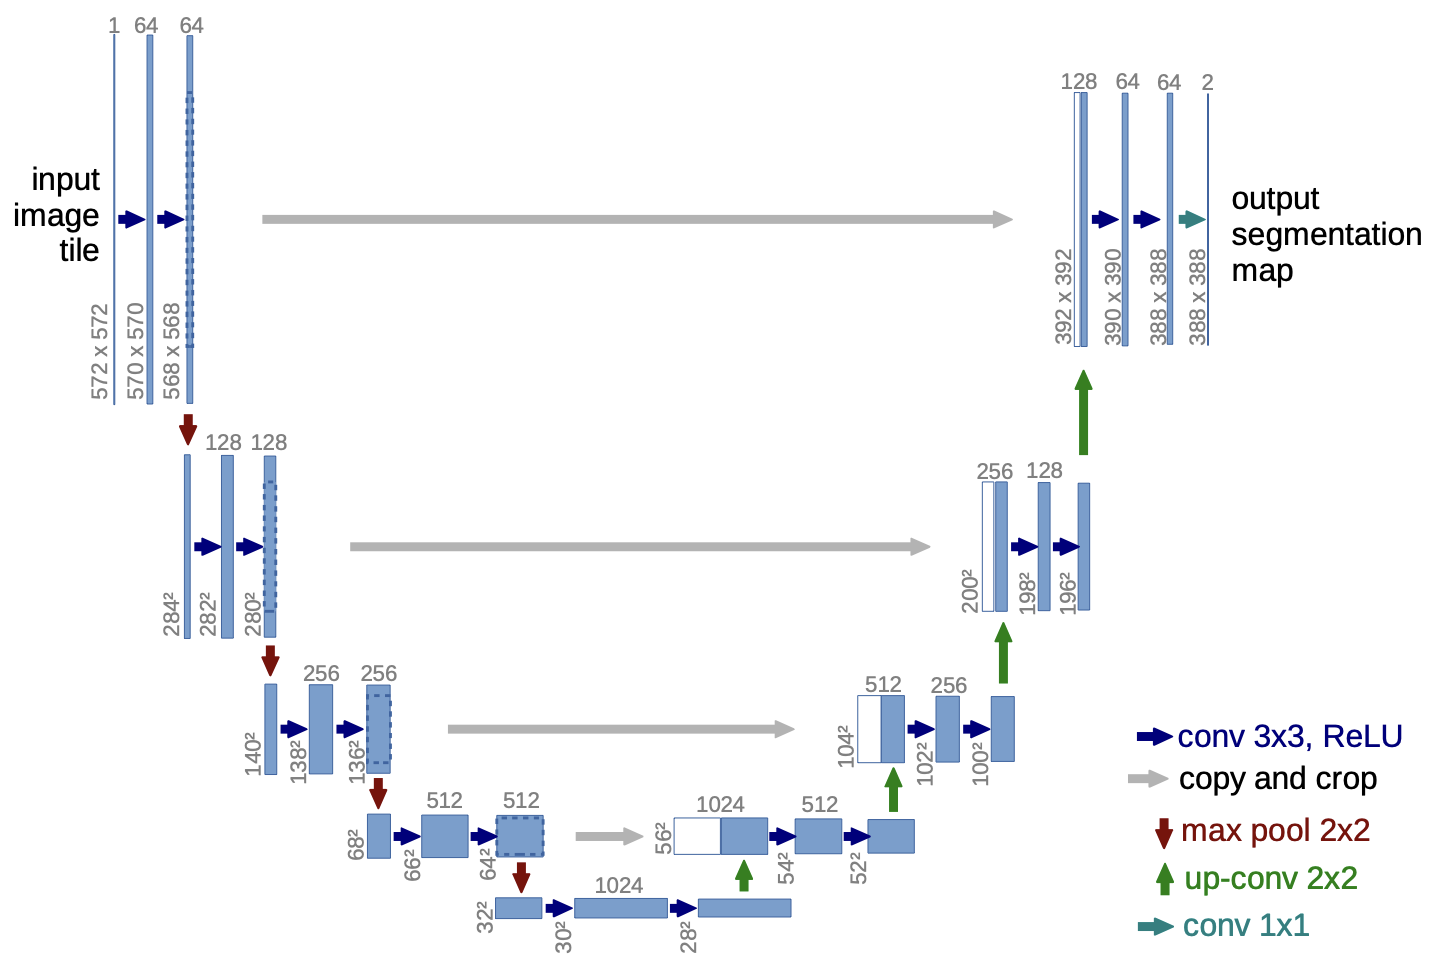
\includegraphics[scale=.5]{figures/unet_paper.png}
	\caption{UNet architecture \cite{ronneberger_u-net_2015}}
	\label{unet architecture}
\end{figure}

In the field of super-resolution data, Akarsh et al. used UNet to upsample the point clouds of mmWave radar \cite{prabhakara_high_2023}. A structure similar to residual path is used in the UNet model, concating the decoder part with the corresponding position of the encoder to alleviate the information loss. The pixel-wise loss and dice loss are combined in the loss function to improve both pixel-wise accuracy and the clarity of the boundary. In the evaluation part, the paper used different environments to test the robustness of the model. Li et al. also applied UNet to the \gls{ra} map collected by \gls{fmcw} radar with \gls{mimo} \cite{li_azimuth_2023}. They have much data processing, inclusive converting the data with the real and imaginary parts, using \gls{fft} to convert the data to a more informative map, and choosing the pixel shuffle method for upsampling.

\begin{spacing}{1.5}
\textbf{\large {Transformer \& Swin Transformer}}
\end{spacing}

In Transformer, the encoder-decoder structure exists as well. There are six identical layers in the encoder part, each layer includes a multi-head attention and a forward propagation sub-layer. According to the attention layer shown in Figure \ref{attention mechanism}, it will calculate the similarity between the query, key and value, thereby obtaining the relationship between different words. In the upsampling task, we will use the self-attention mechanism, that is, query, key and value all come from the same data, thereby obtaining the relationship between the patches. It is on this basis that the \gls{swin} transformer adds shifted windows to achieve that there can be overlapping between windows to improve the uncertainty brought about by fixed split \cite{liu_swin_2021}. Liang et al. proposed the \gls{swinir} architecture based on the \gls{swin} transformer, adding shallow feature extraction and \gls{hq} image restoration \cite{liang_swinir_2021}. The \gls{lq} image will be downsampled once and then passed through multiple \gls{swin} transformers and residual blocks to improve the image resolution.

\begin{figure}
	\centering
	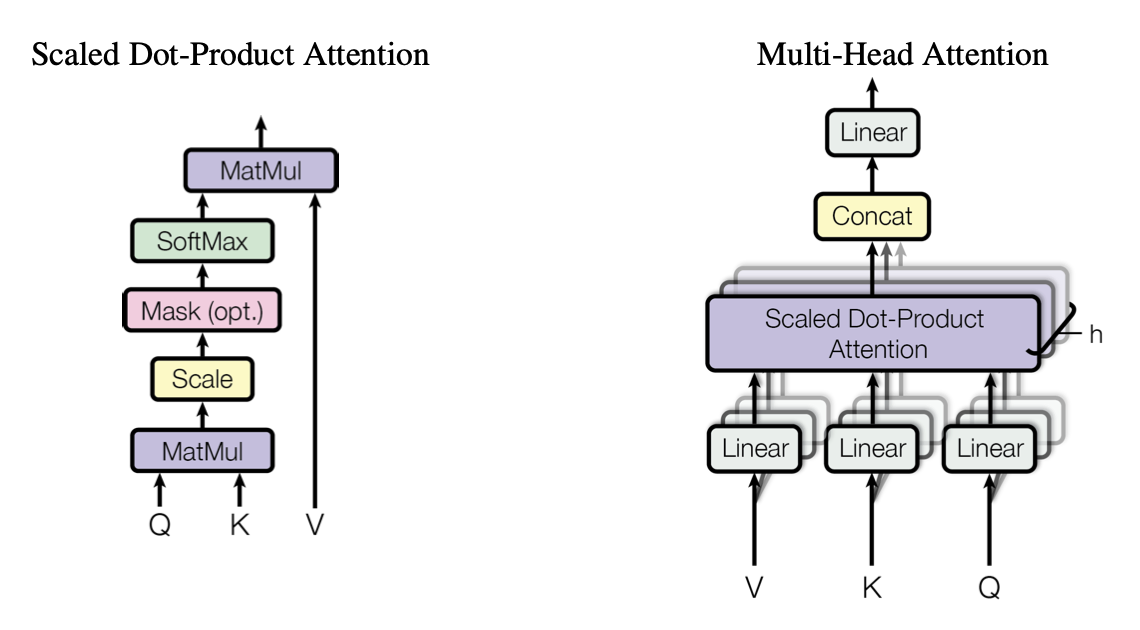
\includegraphics[scale=.65]{figures/attention.png}
	\caption{Attention mechanism \cite{vaswani_attention_2023}}
	\label{attention mechanism}
\end{figure}

The author of \cite{hinderer_blind_2022} proposed a novel approach to separate two signals, which also uses Transformer model, but split the signals along the two coordinates of time and frequency respectively. In addition, due to two signals, it uses a dual-path structure to achieve better distinction between different signal sources. Inspired by this division method, since there are also two obvious dimensions in the range-Doppler map, namely the range and the Doppler effect, we can also try to apply Transformer along these two axes respectively, and the overlapping will exist in this segmentation approach as well.

\begin{spacing}{1.5}
\textbf{\large{GAN \& cGAN models}}
\end{spacing}

The \gls{gan} model also contains two parts, called generator and discriminator. The generator part will extract and learn the data distribution of the input. After generating an output, the discriminator estimates the probability of real and generated samples belonging to the real class. The goal is to make the output of generator as visually close to the ground truth as possible. On the other hand, it is hoped that the discriminator can enhance its discrimination ability and jointly improve the learning ability of the model through adversarial learning between these two parts \cite{goodfellow_generative_2014}.

Based on the \gls{gan} model, Mehdi et al. proposed a conditional version of \gls{gan} model, called \glsfirst{cgan} \cite{mirza_conditional_2014}. \gls{cgan} will feed additional data in the generator and discriminator parts, which is called the condition, as the "y" demonstrated in the Figure \ref{cgan illustrated architecture}. While in our case, the input of the generator is just the low-resolution data as the condition without the noise part. The discriminator will give the probability between the generated super-resolution and real high-resolution range-Doppler maps based on the conditional low-resolution range-Doppler map, which is well shown in Figure \ref{cgan architecture without noise for the generator}.

\begin{figure}
	\centering
	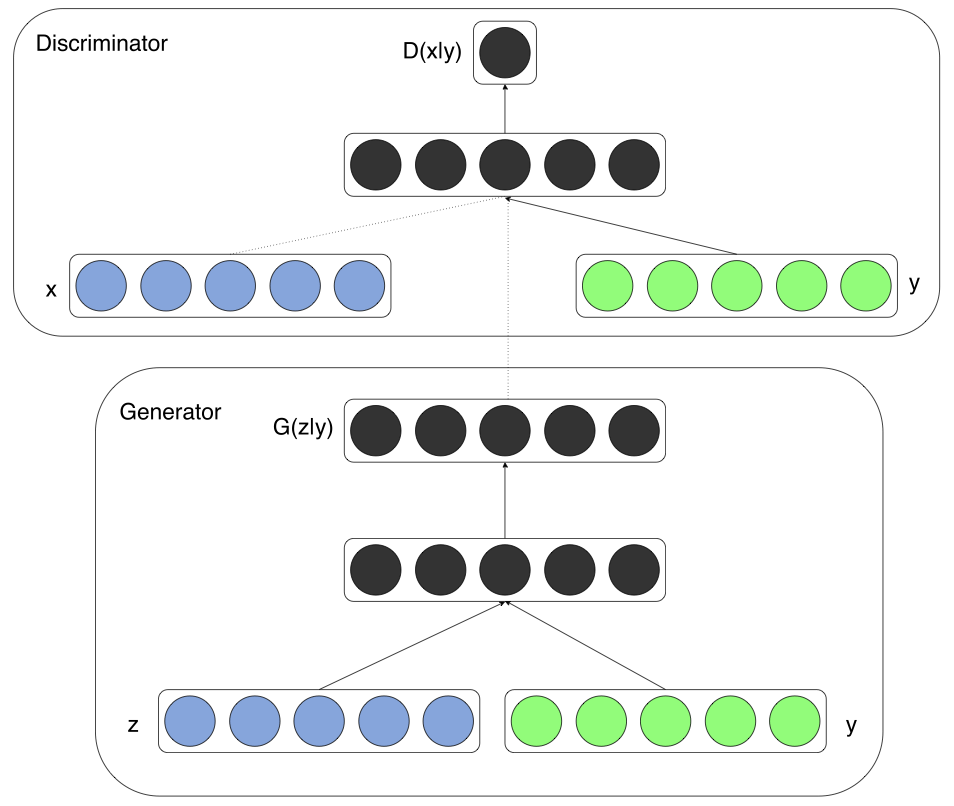
\includegraphics[scale=.65]{figures/cgan_paper.png}
	\caption{cGAN architecture, where x is the ground truth or the generated output, z represents the noise and y is the condition of the model \cite{mirza_conditional_2014}.}
	\label{cgan illustrated architecture}
\end{figure}

\begin{figure}
	\centering
	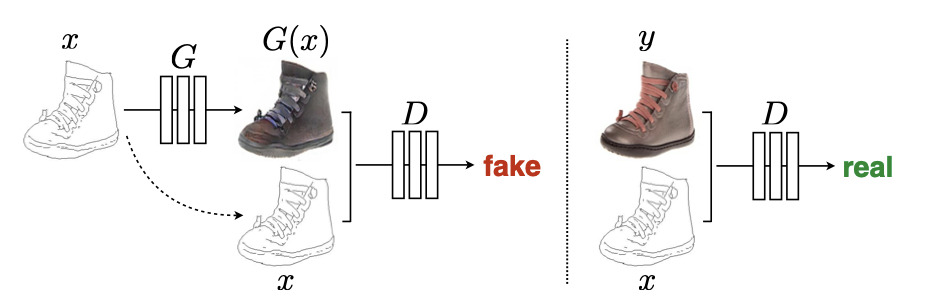
\includegraphics[scale=.8]{thesis/figures/cgan_pix2pix.png}
	\caption{cGAN architecture without noise input for the generator, where x is the conditional low-resolution data and y is the ground truth \cite{isola_image--image_2018}.}
	\label{cgan architecture without noise for the generator}
\end{figure}

In the field of image super-resolution remedy, Karim et al. used the \gls{gan} model on the data of \gls{fmcw} radar, which was based on the micro-Doppler signature of walking human targets \cite{armanious_adversarial_2019}. The \gls{gan} model consists of two parts: the discriminator and the CasNet generator, where the CasNet generator is a stack of multiple UNet models. The loss function combines the pixel-wise L1 loss and the perceptual loss obtained by the discriminator. Compared with the task in this thesis, the content of our range-Doppler map is more complicated and the dynamic range of the data is more obvious.

With the usage of \gls{cgan}, Kong applied it to the super-resolution of \gls{sar} imagery \cite{kong_dmsc-gan_2023}. The structure of UNet is used in the generator, downsampling is performed through the convolutional layer and upsampling is performed through transposed convolutional layer, and an attention mechanism is performed after each dimension change. Furthermore, multiple losses are combined in the loss function, including \gls{gan} loss, VGG perceptual loss and feature matching loss. Inspiration from this, multiple loss functions can also be combined in our training process to achieve better results. Sherif et al. used the \gls{cmgan} model, combining the Transformer with the GAN structure to learn long-distance dependencies and the convolutional layers to exploit local features, which can tackle a variety of tasks, including super-resolution processing of speech \cite{abdulatif_cmgan_2024}.

Also in the field of super-resolution range-Doppler map, Jeong et al. used the \gls{cgan} architecture, in which the generator was based on the UNet model \cite{jeong_resource-efficient_2023}. In the evaluation, more metrics are used, such as \gls{pmse}, \gls{psnr}, etc. However, since the data was collected mainly in open areas such as the playground, the content in the range-Doppler map is relatively simple. Ledig et al., in their SRGAN model, a GAN for super-resolution image, used a larger resampling rate, namely factor of four, which puts higher requirements on the ability of the model \cite{ledig_photo-realistic_2017}. Meanwhile, they combine perceptual loss, adversarial loss and content loss to prevent the loss of high-frequency information and ensure that the boundaries of objects are clear.


\chapter{Dataset} \label{dataset}
Dataset is very important for the training. Sufficient data that meets the requirement of the task is crucial, and the proper preprocessing can effectively help the model learn well. Based on the complexity of the indoor environment, which leads to the wide dynamic range of the data amplitude, we choose to collect the required dataset by ourselves so that the model can better adapt to complex range-Doppler map.

\section{Dataset recording} \label{dataset recording}
% The hardware of the radar product, the parameters, settings of recording, the environment and environment split, and the size of the dataset as well as resampling.

\begin{spacing}{1.5}
\textbf{\large{Radar hardware}}
\end{spacing}

In the collection of the dataset, we used the type of BGT60TR13C radar from Infineon \cite{ag_bgt60tr13c_nodate}. The BGT60TR13C type is a 60 GHz radar sensor with four integrated antennas, which includes single \gls{tx} and three \glspl{rx}, where the receivers are arranged in L-shape as shown in Figure \ref{the antenna arrangement of the radar}. In the task, due to the single channel chirp sequence radar, one of the three receivers has to be chosen. \gls{rx}3 is used by default during the recording, since \gls{rx}1 and \gls{rx}2 are closer to the \gls{tx} than Rx3, it means that the interference between signals will increase, and the noise will increase accordingly. On the other hand, using different receivers can increase the variety of data to a certain extent, so \gls{rx}1 is also sometimes used in the collection process.

\begin{figure}
	\centering
	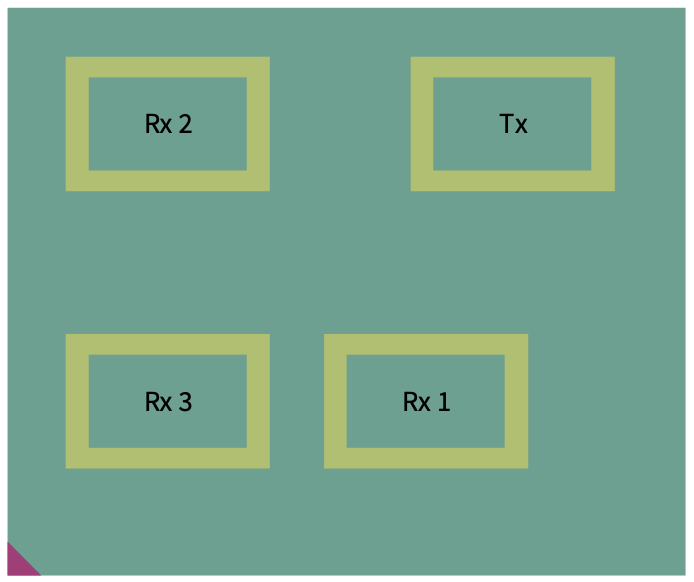
\includegraphics[scale=.5]{thesis/figures/antenna arrangement.png}
	\caption{The antennas arrangement of the radar device \cite{ag_bgt60tr13c_nodate}}
	\label{the antenna arrangement of the radar}
\end{figure}

The advantage of the BGT60TR13C radar is that it can achieve ultra-wide bandwidth \gls{fmcw} operation in a small package, which is conducive to provide higher resolution, retain more details and provide more possibilities in data, such as the downsample as the factor of 4. With a bandwidth of 5.5 GHz, the minimum range resolution is \SI{3}{\centi\meter}. Furthermore, the high \gls{snr} of this radar can achieve detection of up to \SI{15}{\meter}, providing a good hardware foundation for the movement, identification and segmentation of objects within this range, where more parameters are given in Table \ref{parametrics of the radar product}.

\begin{table}
    \centering
    \caption{Parameters of the BGT60TR13C radar product \cite{ag_bgt60tr13c_nodate}}
    \label{parametrics of the radar product}
    \begin{tabular}{cc|cc}
        \hline
        \multicolumn{1}{l|}{Parametrics} & BGT60TR13C & \multicolumn{1}{l|}{Parametrics} & BGT60TR13C \\
        \hline
        \multicolumn{1}{l|}{Angle of Arrival} & Yes & \multicolumn{1}{l|}{Current consumption} & 200 mA \\
        \hline
        \multicolumn{1}{l|}{Motion} & Yes & \multicolumn{1}{l|}{Supply voltage} & 1.8 V \\
        \hline
        \multicolumn{1}{l|}{Frequency} & 60 GHz & \multicolumn{1}{l|}{Gain} & 5 dBi \\
        \hline
        \multicolumn{1}{l|}{Min. frequency} & 58 GHz & \multicolumn{1}{l|}{Max detection range} & 15 m \\
        \hline
        \multicolumn{1}{l|}{Max. frequency} & 63.5 GHz & \multicolumn{1}{l|}{Min detection range} & 0.2 m \\
        \hline
        \multicolumn{1}{l|}{Range} & Yes & \multicolumn{1}{l|}{Speed} & Yes \\
        \hline
        \multicolumn{1}{l|}{Number of Rx antennas} & 3 & \multicolumn{1}{l|}{Number of Tx antennas} & 1 \\
        \hline
        % \multicolumn{1}{l|}{Minimal required TX power ($\mu \mathrm{W}$)} & 0.99 & 1.91 & 2.49 & 2.94 & 4.32\\
    \end{tabular}
\end{table}

While using this BGT60TR13C radar, Infineon provides a corresponding radar \gls{sdk}, which can access radar sensors and collect data through C/C++, Python and MATLAB, and can implement some radar algorithms such as range-Doppler map, simple segmentation, etc. with the \gls{sdk}. In addition, Infineon also provides wrappers that adapt to multiple platforms, such as MacOS, Linux, etc. For specific instructions, the developer community and other platforms can be referred \cite{noauthor_how_2023}.

\begin{spacing}{1.5}
\textbf{\large{Initial device parameters}}
\end{spacing}

The parameters and settings during the data collection are mainly divided into three parts: the initial parameter settings of the radar, the time interval during radar operation, and the environmental conditions for collection. This part is about the parameters derivation of the radar.

As a member of Infineon's 60 GHz family, the wavelength $\lambda$ of this radar is
\begin{equation}
    \centering
    \lambda = \frac{c}{f} = 5\,\mathrm{mm}.
\end{equation}

According to the information in Table \ref{parametrics of the radar product}, the bandwidth range is selected from 59 GHz to 63 GHz, that is, the bandwidth is 4 GHz. Since the collected range-Doppler map is mainly based on the indoor environment, the maximum velocity requirements are not that high, and it can be within $\pm$5 m/s. Therefore, according to the relationship between \gls{cri} $T_p$ and maximum velocity $v_{max}$, the required \gls{cri} can be obtained as
\begin{equation}
    \centering
    T\textsubscript{p} = \frac{\lambda}{4 \cdot v\textsubscript{max}} = 2.5 \times 10^{-4}\,\mathrm{s}.
\end{equation}

Considering the requirements of velocity resolution, data processing capability, and power consumption, the chirp repetition interval is determined as $T_p$=220 \textmu s. Conversely, the detectable velocity is
\begin{equation}
    \centering
    v\textsubscript{max} = \frac{\lambda}{4 \cdot T\textsubscript{p}} = 5.68\,\mathrm{m/s}.
    \label{maximum velocity equation}
\end{equation}

$T_p$ is usually a little larger than the duration of the chirp $T_c$ to make sure that there will a gap between chirps. This ratio is usually set as 1.1, that is, $T_c$=200 \textmu s.

If the detection range is too large, the radar power and resolution will be more demanding, and the noise will also increase. Assuming that the maximum range is set at roughly \SI{10}{\meter}, the relationship between the number of samples $N_s$ and the maximum range $r_{max}$ can be obtained as
\begin{equation}
    \centering
    N\textsubscript{s} = \frac{2B \cdot r\textsubscript{max}}{c} = \frac{2 \cdot 4\,\mathrm{GHz} \cdot 10\,\mathrm{m}}{3 \times 10\textsuperscript{8}\,\mathrm{m/s}} = 266.67.
\end{equation}

Since the \gls{fft} operation is most efficient while processing data is the power of 2, the number of chirp $N_s=256$. Due to the real-valued data collected by the radar, the negative frequencies will be discarded by the \gls{rfft} processing, the required sampling number should be doubled to $N_s=512$. Therefore, the maximum range is specified as 
\begin{equation}
    \centering
    r\textsubscript{max} = \frac{c \cdot N\textsubscript{s}}{2B} = 9.6\,\mathrm{m}.
    \label{maximum range equation}
\end{equation}

According to the number of samples and chirp time, the sampling frequency $F_s$ can be deduced as
\begin{equation}
    \centering
    F\textsubscript{s} = \frac{N\textsubscript{s}}{T\textsubscript{c}} = \frac{512}{200 \times 10^{-6}\,\mathrm{s}} = 2.56\,\mathrm{MHz}.
    \label{sampling frequency equation 2.6}
\end{equation}

The number of chirps is limited by the velocity and range resolution as well as the maximum velocity. If the required velocity resolution $\Delta v$ and the range resolution $\Delta r$ are set to be no less than 0.2 m/s and \SI{0.2}{\meter} respectively, the number of chirps $N_c$ will be limited by two values, namely between
\begin{equation}
    \centering
    N\textsubscript{c} \geq \frac{c}{2f\textsubscript{c}} \cdot \frac{1}{T\textsubscript{p} \cdot \Delta v} = \frac{3 \times 10\textsuperscript{8}\,\mathrm{m/s}}{2\cdot 60\,\mathrm{GHz} \cdot 220\,\text{\textmu s} \cdot 0.2\,\mathrm{m/s}} = 56.82,
\end{equation}
and
\begin{equation}
    \centering
    N\textsubscript{c} \leq \frac{\Delta r}{2 \cdot v\textsubscript{max} \cdot T\textsubscript{p}} = \frac{0.2\,\mathrm{m}}{2\cdot 5.68\,\mathrm{m/s} \cdot 220\,\text{\textmu s}} = 80.03.
\end{equation}

Similarly as the reason for $N_s$, the number of chirps will be determined as $N_c=64$.

\begin{table}
    \centering
    \caption{Initial configs of the radar device, where the resolutions are calculated in the section \ref{dataset loading}.}
    \label{initial configs of the radar device}
    \begin{tabular}{l|c|l|c}
        \hline
        \textbf{Parametrics} & \textbf{Value} & \textbf{Parametrics} & \textbf{Value} \\
        \hline
        Chirp repetition time $T_p$ & 220 \textmu s & Frequency $f$ & 60 GHz \\
        \hline
        \#Chirps $N_c$ & 64 & \#Samples $N_s$ & 512 \\
        \hline
        Start frequency $f_{c}$ & 59 GHz & End frequency $f_{max}$ & 63 GHz \\
        \hline
        Sample rate $F_{s}$ & 2.56 MHz & Gain $G$ & 33 dB \\
        \hline
        Receiver index & 1 or 3 & Transmitter index & 1 \\
        \hline
        Maximum range $r_{max}$ & 9.6 m & Maximum speed $v_{max}$ & 5.68 m/s \\
        \hline
        Range resolution $\Delta r$ & 0.0375 m & Velocity resolution $\Delta v$ & 0.178 m/s \\
        \hline
    \end{tabular}
\end{table}

In summary, the initial parameters of the radar can be set according to Table \ref{initial configs of the radar device}. In the process of data collection, in order to mitigate the correlation between the scene and the surrounding objects, we increased the time interval. Specifically, the data collected once in the above initial setting is called a frame, the interval between frames will be a little bit increased, namely 0.1 second, and each group will include 8 frames. This setting can ensure the motion coherence of the object related to the radar while the similarity of the data can be mitigated.

To further reduce the similarity between groups, the time interval between groups is set as 1 second, and 5 groups are collected each time. The above process is considered to be called as the single measurement or called once measurement. The interval between each measurement is also set as 1 second. During the time interval between two measurements, the position and angle of the radar will change significantly. The direction of the radar is not limited to the ceiling, but also faces all surroundings, except the floor. This recording setting is summarized in the Table \ref{recording settings}.

\begin{table}
    \centering
    \caption{Recording settings}
    \label{recording settings}
    \begin{tabular}{l|c}
        \hline
        \textbf{Settings} & \textbf{Value} \\
        \hline
        Repetition interval between frames & 0.1 s \\
        \hline
        \#Frames & 8 \\
        \hline
        Interval between groups & 1 s \\
        \hline
        \#Groups & 5 \\
        \hline
        Interval between the measurements  & 1 s \\
        \hline
    \end{tabular}
\end{table}

\begin{spacing}{1.5}
\textbf{\large{Environment}}
\end{spacing}

During the data collection process, the data was mainly recorded in the indoor environment, and the location was in the corridor of the V47 building at the University of Stuttgart. Compared with dynamic data, static data does not provide more information, but loses the information of the Doppler effect, which will not improve the model much. Therefore, only dynamic data exists in the data collection process. Data is collected by walking between the five floors from -1 to 4, and other students and scholars will also pass through the corridor at the same time, which will enrich the data content to a certain extent.

The equipments used in the recording are mainly the laptop and the radar. The dataset which is recorded in the first time, i.e. \texttt{dataset\_1}, the laptop was moved by placing it on a chair with sliding wheels, while in subsequent data measurements, the laptop was directly carried in a backpack. Hence, the data collection process includes two tempos, called medium tempo and slow tempo. The medium tempo means the normal walking velocity of an adult, and the slow tempo includes the data measured when the walking speed is slowed down or the chair is pushed. In conclusion, the environmental conditions of the recording are summarized in Table \ref{environment conditions}.

\begin{table}
    \centering
    \caption{Environment conditions}
    \label{environment conditions}
    \begin{tabular}{c|c|c|c}
    \hline
    \multicolumn{2}{c|}{\textbf{Type}} & \textbf{Environment} & \textbf{Tempo} \\
    \hline
    \multirow{2}{*}{Dynamic} & \multirow{2}{*}{Indoor} & \multirow{2}{*}{Corridors of building V47} & Medium tempo\\
    \cline{4-4}
    & & & Slow tempo \\
    \hline
    \end{tabular}
\end{table}

\begin{spacing}{1.5}
\textbf{\large{Dataset structure}}
\end{spacing}

In the server, the data is stored in the path \texttt{/data/public/rd\_sr/}. There are currently three folders, which also represent three types of data. As the earliest data, \texttt{dataset\_sample} has most of its data in a static state, and the number of chirps and samples are relatively lower, which is not enough for resampling, so it is abolished. The above parameters in Table \ref{initial configs of the radar device} are firstly used in \texttt{dataset\_1}, but the data is still divided into dynamic and static, as well as the environments in different rooms. Subsequently, the sampling parameters and environment set in the above tables are used in \texttt{dataset\_2}. On this basis, the dynamic and in corridor collected part of \texttt{dataset\_1} is taken into the low tempo case of the \texttt{dataset\_2}. Then, the following entire subsequent data processing and training parts will only use the data in \texttt{dataset\_2}.

In \texttt{dataset\_2}, the following structure is the subfolders of the environment and tempo, the next are the measurements, five groups and eight frames of data in each group. The naming convention for each measurement is, in order, the location (such as corridor), mode (such as moving radar), year, month, day, hour, minute and second, connecting with the underlines. Following illustrates the view of the data storage structure.
\dirtree{%
 .1 /data/public/rd\_sr/.
 .2 dataset\_sample/.
 .3 .../.
 .2 dataset\_1/.
 .3 .../.
 .2 dataset\_2/.
 .3 corridor/.
 .4 medium\_tempo/.
 .5 .../.
 .4 slow\_tempo/.
 .5 Corridor\_movingRadar\_2024\_12\_17\_16\_50\_3/.
 .5 .../.
 .5 .../.
 .5 Corridor\_movingRadar\_2024\_12\_17\_16\_52\_4/.
 .6 0/.
 .7 ....
 .6 .../.
 .6 5/.
 .7 0.pickle.
 .7 1.pickle.
 .7 ....
 .7 8.pickle.
}

\begin{spacing}{1.5}
\textbf{\large{Size}}
\end{spacing}

In \texttt{dataset\_2}, the medium tempo includes 1431 measurements, and the low tempo includes 931 measurements. The size of \texttt{dataset\_2} reaches 16.4 GB totally.

In the way of splitting dataset, since the scene only occurs in the corridor, the training set, validation set and test set will be divided according to the tempo. Assuming that the training set and validation set contain both medium tempo and low tempo, and the test set only contains medium tempo, the medium tempo part will be divided into 80\% for the training process and 20\% for the test set, and of the 80\%, 80\% will be divided into the training set and 20\% into the validation set. 80\% of the low tempo part will be divided into the training set and 20\% into the validation set. According to the above mentioned division method, the training set can contain 11.9 GB data, the size of validation set will be roughly 3 GB, while the size of test set is 1.5 GB.

\section{Dataset loading} \label{dataset loading}
% the settings \& Creation of the \gls{tfrecord} files creation such as frame of length, shift window for augmentation, cube de-biasing, iFFT, FFT shift, riFFT.

For dataset loading, we will read and store it in \gls{tfrecord} files to effectively speed up the training process, and directly reload the \gls{tfrecord} files in the subsequent training process. During creating \gls{tfrecord} files, the number of frames and resampling operation will be done, and the conversion between the frequency domain and time domain will be performed in the subsequent reloading process.

\begin{spacing}{1.5}
\textbf{\large{\gls{tfrecord} files}}
\end{spacing}

\gls{tfrecord} is a file format based on the TensorFlow framework that stores data in binary format. This data format can bring many benefits, one of which is that it helps to speed up the training efficiency and reduce the waiting time for data loading of each training process. Since the subfolders must be loaded in sequence, the process of loading the subfolders needs to be completed by the CPU, which will increase the requirements for the CPU and CPU memory, as well as the time required, while the \gls{tfrecord} files reloading process can be operated by the GPU which allows the parallel \gls{i/o} operations. According to a rough estimation, it will take nearly 3 hours to complete all data loading, while only costs roughly 5 minutes to reload it from the \gls{tfrecord} files. However, note that the durations are still depending on the usage of server resources or settings.

Another advantage is that due to its binary format, it can effectively reduce the space of the data storage. According to the estimated size of the ground truth in the training set, validation set, and test set in section \ref{dataset recording}, it can reach 11.9 GB, 3 GB, and 1.5 GB respectively. On this basis, the corresponding low-resolution data will also be saved in the \gls{tfrecord} files. Table \ref{advantages of the tfrecord files} shows the space occupied by saving both low-resolution and high-resolution data after downsampling by the factor of two and four. The occupied storage space is much smaller.

\begin{table}
    \centering
    \caption{Advantages of the TFRecord files about loading time and storage space, where the TFRecord files of resampling with the factor 2 or 4 contain both low-resolution and high-resolution data while in the original data folders only the high-resolution data is stored. Note that the durations is still depending on the usage of server resources.}
    \label{advantages of the tfrecord files}
    \begin{tabular}{cccc}
        \hline
        \multicolumn{4}{c}{\textbf{Duaration of the dataset loading}}\\
        \hline
        \multicolumn{2}{l|}{Loading the subfolders} & \multicolumn{2}{c}{\textasciitilde 3 hours}\\
        \hline
        \multicolumn{2}{l|}{Loading the \gls{tfrecord} files} & \multicolumn{2}{c}{\textasciitilde 5 minutes}\\
        \hline
        \multicolumn{4}{c}{\textbf{Storage of the dataset}}\\
        \hline
        \multicolumn{1}{l|}{Type} & \multicolumn{1}{c|}{High resolution data} & \multicolumn{1}{c|}{Factor of 2} & \multicolumn{1}{c}{Factor of 4}\\
        \hline
        \multicolumn{1}{l|}{Train set} & \multicolumn{1}{c|}{11.9 GB} & \multicolumn{1}{c|}{5.6 GB} & \multicolumn{1}{c}{3.5 GB}\\
        \hline
        \multicolumn{1}{l|}{Validation set} & \multicolumn{1}{c|}{3 GB} & \multicolumn{1}{c|}{1.4 GB} & \multicolumn{1}{c}{888 MB}\\
        \hline
        \multicolumn{1}{l|}{Test set} & \multicolumn{1}{c|}{1.5 GB} & \multicolumn{1}{c|}{717 MB} & \multicolumn{1}{c}{448 MB}\\
        \hline
    \end{tabular}
\end{table}

There are two processes of the \gls{tfrecord} files, namely creating and reloading. Firstly, in the process of creating files, the subfolders are read in sequence. In the code pipeline, a combination of dictionaries and lists is used to store data. The first-hierarchy of the dictionary records the environment and low- or high-resolution data. Although the current data only has the environment of indoor corridors, it is prepared for the case of new environments in the future. Each dictionary adds the same number of lists according to the number of tempo types, which corresponds to the structure in Table \ref{environment conditions}, so as to facilitate the subsequent split according to the required types in different dataset. To clarify it, according to the current corridor environment, two dictionaries will be generated, called \texttt{corridor\_GT} and \texttt{corridor\_downsampled}, and then each dictionary will contain two lists, called \texttt{medium\_tempo} and \texttt{slow\_tempo}.

For any list in \texttt{corridor\_GT}, its size will be \texttt{(\#Sequences, 1, 64, 512)} while \texttt{corridor\_downsampled} with factor of two has the size of \texttt{(\#Sequences, \#Frames, 32, 256)}. Therefore, in the current pipeline, two parameters in the \gls{tfrecord} file will be determined, one is the number of frames and the other is the resampling rate. The significance of the number of frames is that due to the continuous motion of the radar, such as feeding 4 consecutive range-Doppler maps for the model, the model learns the temporal correlation between consecutive range-Doppler maps and creates more consistent outputs, while the input with single range-Doppler map doesn't have this information. Based on this goal, a sliding window approach will be introduced in loading for data augmentation which will be explained following. In the \gls{tfrecord} files, except the low-resolution and high-resolution data being stored in byte format, the corresponding sizes of the two dictionaries are stored as int value for subsequent reloading. Additionally, the data cube will be operated with the de-biasing to remove the offset of each chirp.

The other part is to prepare the data from the \gls{tfrecord} files, and after restoring the data according to the size stored in the \gls{tfrecord} files, some additional processing will be performed. First of all, \gls{rdp} will be used to convert the real-valued cube in the time domain into the complex-valued data in the frequency domain, and the minimum, mean as well as maximum values of the each dataset will be calculated for normalization, which will be shown in section \ref{normalization types}, then they will be split into mini-batches, additionally the training set will be shuffled.

\begin{spacing}{1.5}
\textbf{\large{Sliding window for the number of frames}}
\end{spacing}

As mentioned above, due to the continuous movement of the radar, the changes in the range and relative velocity of the objects can have some relationships. When the data also contains previous information, the upsampling results of the model could be better. This part of the evaluation will be shown in the section \ref{FOL comparison}. Two settings about the number of frames can be evaluated, namely a single frame without previous information and four frames. The quantity and quality of data will have a great impact on the training process of the model. In order to augment the data, the sliding window will be used, as shown in Figure \ref{sliding window}.

\begin{figure}
    \centering
    \hspace{-0.4cm}
    \begin{subfigure}{0.49\textwidth}
        \centering
        \adjustbox{height=3.2cm}{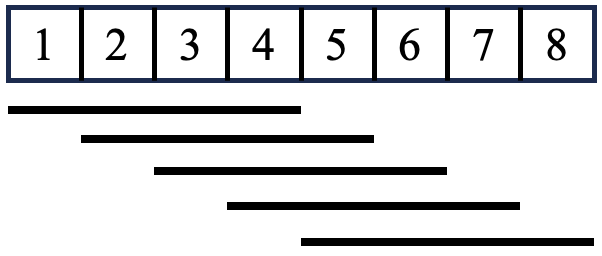
\includegraphics[scale=.24]{thesis/figures/sliding_window_left.png}}
        \caption{Shift step as one}
        \label{shift step as one}
    \end{subfigure}
    \begin{subfigure}{0.49\textwidth}
        \centering
        \adjustbox{height=3.2cm}{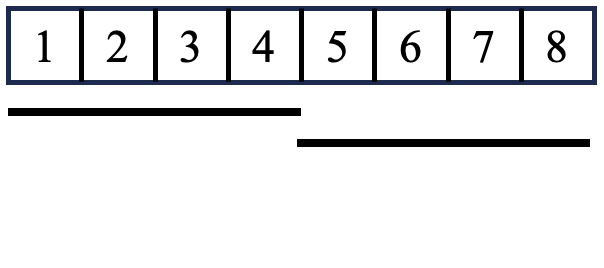
\includegraphics[scale=.24]{thesis/figures/sliding_window_right.png}}
        \caption{Stride same as the number of frames}
        \label{shift step as the fol value}
    \end{subfigure}
    \caption{Sliding window while the number of the frames is 4, where the number 1-8 represent the frames in each group and the lines illustrate the selected frames within each window.}
	\label{sliding window}
\end{figure}

According to the measurement, group and frame defined in Table \ref{recording settings}, the sliding window will only be applied to the frames, that is, sliding within each group. That is to say, the integers from 1 to 8 in Figure \ref{sliding window} above represent the pickle files stored in eight frames, namely \texttt{1.pickle} to \texttt{8.pickle}. The reason for applying it only within the group is that in the above recording setting, in order to reduce the similarity of the scenery and data, the time interval between groups and collections is larger, so only the data within each group can be regarded as continuous. The lines at the bottom of the figures represent the frames covered by the window. The four frames covered will be used as one sequence input of the model, and the data to be upsampled is the last frame within each window, and the ground truth is only the high-resolution version of this last frame.

In addition, there are two ways as shown in Figure \ref{sliding window}. The window in Figure \ref{shift step as one} moves once a step, while the window in Figure \ref{shift step as the fol value} moves according to the number of frames. Compared with the approach that only loads the certain required number of frames once within a group, the method in Figure \ref{shift step as the fol value} will obtain twice the amount of data, while Figure \ref{shift step as one} can obtain five times the amount. However, the shift method in the Figure \ref{shift step as one} will cause the overlapping part, that is, the data to be upsampled in one input also appears in another input, which blows up the scale of the dataset but doesn't bring more information. Therefore, in order to ensure the quality of the data, subsequent data processing will only use the window sliding in the way as in Figure \ref{shift step as the fol value}.

\begin{spacing}{1.5}
\textbf{\large{Resampling}}
\end{spacing}

During creating the \gls{tfrecord} files, high-resolution and low-resolution data will be stored in pairs. At this moment, the data is still in the time domain. Figure \ref{downsample in time domain with the factor of 2} draws a signal containing multiple chirps and the process of the downsampling with the factor of two.

\begin{figure}
	\centering
	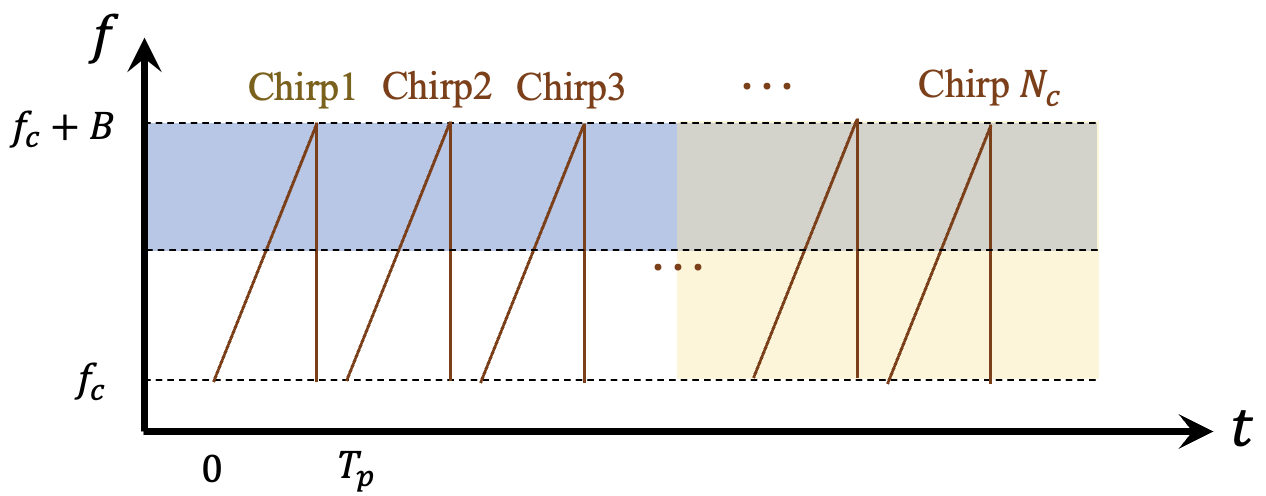
\includegraphics[scale=.67]{thesis/figures/resampling.png}
	\caption{Downsampling processing with the factor of 2 by cutting the bandwidth with only half samples within the chirp to obtain half range resolution and dropping half of the chirps to halve the velocity resolution.}
	\label{downsample in time domain with the factor of 2}
\end{figure}

Based on the radar settings selected above, the velocity and range resolutions can be calculated separately. Substituting the initial radar parameters from into the velocity resolution formula below, the value is
\begin{equation}
    \centering
    \Delta v = \frac{c}{2f\textsubscript{c}} \cdot \frac{1}{T\textsubscript{p} \cdot N\textsubscript{c}} = 0.178\,\mathrm{m/s},
    \label{velocity resolution equation}
\end{equation}

while the range resolution can be derived as
\begin{equation}
    \centering
    \Delta r = \frac{c}{2B} = 0.0375\,\mathrm{m}.
    \label{range resolution equation}
\end{equation}

First of all, regarding the resampling of velocity resolution, according to the derivation of formula \ref{velocity resolution equation}, if in order to double the velocity resolution while the speed of light and carrier frequency are constant, the \gls{cri} $T_p$ or the number of chirps $N_c$ have to be reduced to half of the original parameters. Since the \gls{cri} have the influence on the shape of chirp and it's hard to build the pairs with different \gls{cri}, the later alternative is chosen, namely the number of chirps $N_c$ turns to 32, corresponding to the abolishment of the signals under the yellow mask in Figure \ref{downsample in time domain with the factor of 2}, and only keep the first 32 chirps. In terms of the range resolution, according to formula \ref{range resolution equation}, since the speed of light is a constant, reducing the bandwidth increases the range resolution. Therefore, the blue mask in Figure \ref{downsample in time domain with the factor of 2} indicates that the upper half of the chirp has been removed, thereby halving the range resolution.

For the maximum values of both velocity and range, according to formulas \ref{maximum velocity equation} and \ref{maximum range equation}, maintaining the wavelength $\lambda$ and \gls{cri} $T_p$ can ensure that the maximum velocity is the same as the high-resolution case. When the bandwidth is reduced by half, the number of sampling points within each chirp is also reduced by half, as plugging the formula \ref{sampling frequency equation 2.6} into the formula \ref{maximum range equation}, the maximum value of the range is up to the slope only, hence, it remains.

For each high-resolution frame within the sliding window, known the shape of each high resolution data is \texttt{(64, 512)}, the pseudo-code of this downsampling process is written in Algorithm \ref{pseudo code of downsampling}.
\begin{algorithm}
    \caption{Pseudo code of resampling}
    \label{pseudo code of downsampling}
    \renewcommand{\algorithmicrequire}{\textbf{Input:}}
    \renewcommand{\algorithmicensure}{\textbf{Output:}}
    
    \begin{algorithmic}[1]
        \REQUIRE $High-resolution\ data\ as\ data,\ sampling\ rate$
        \ENSURE $Low-resolution\ data$

        \STATE $row\ =\ data.shape[0]$
        \STATE $col\ =\ data.shape[1]$
        \STATE $low\_resolution\_data\ =\ data[:row\ //\ sampling\_rate,\ :col\ //\ sampling\_rate]$
        
    \end{algorithmic}
\end{algorithm}

\begin{spacing}{1.5}
\textbf{\large{Cube de-biasing}}
\end{spacing}

During creating the \gls{tfrecord} files, another operation is cube de-biasing. Cube de-biasing refers to the mean removal of the data cube. The main purpose of this operation is to eliminate the constant offset caused by the hardware system or environment, so as to more clearly and fairly detect the reflected signal of the target, while ensuring no different offset between the chirps in the collection process.

The operation of cube de-biasing is to calculate the mean of each chirp, and then expand it to the size of $N_s$ to remove the offset along the fast time axis. The pseudo code is as following Algorithm \ref{pseudo code of cube de-biasing}.
\begin{algorithm}
    \caption{Pseudo code of cube de-biasing}
    \label{pseudo code of cube de-biasing}
    \renewcommand{\algorithmicrequire}{\textbf{Input:}}
    \renewcommand{\algorithmicensure}{\textbf{Output:}}
    
    \begin{algorithmic}[1]
        \REQUIRE $Cube\ data\ in\ time\ domain$
        \ENSURE $Debiasing\ data$

        \STATE $avgs\ =\ np.average(cube,\ 1)[:,\ None]$
        \STATE $cube\ =\ cube\ -\ avgs$
        
    \end{algorithmic}
\end{algorithm}

\begin{spacing}{1.5}
\textbf{\large{\gls{rdp}}}
\end{spacing}

After loading the \gls{tfrecord} files, one processing to do is \gls{fft}, which is used to convert the data from time domain to frequency domain. This is a very important process in radar signal processing. Decomposing the data in the time domain into different frequency components helps to provide more useful information.

But in \gls{fft}, the frequency can be positive or negative, since the sine and cosine signals in the complex component can be in both directions. However, in our radar data, the signal in time domain is real-valued, which is different from the complex-valued signal as input. The real-valued input signal has a Hermitian symmetric spectrum. The reason is that in the definition of \gls{fft}, for a discrete signal $x(n)$ with the length of $N$, its \gls{dft} conversion is as following
\begin{equation}
    \centering
    X[k] = \sum_{n=0}^{N-1} x[n] e^{-j\frac{2\pi kn}{N}}.
\end{equation}

Its conjugate is
\begin{equation}
    \centering
    X^*[k] = \sum_{n=0}^{N-1} x[n] e^{+j\frac{2\pi kn}{N}},
\end{equation}

then they both can be derived as conjugated pair, namely
\begin{equation}
    \centering
    X[N - k] = X^*[k].
\end{equation}

Therefore, there is no additional information between the positive and negative parts, in order to reduce the computational complexity and storage requirements, we can only save the information of the positive frequency part as well as one real value and discard the negative frequency part. Figure \ref{an overview of the rfft} shows well the finally obtained symmetrical data after the \gls{fft} process.

\begin{figure}
	\centering
	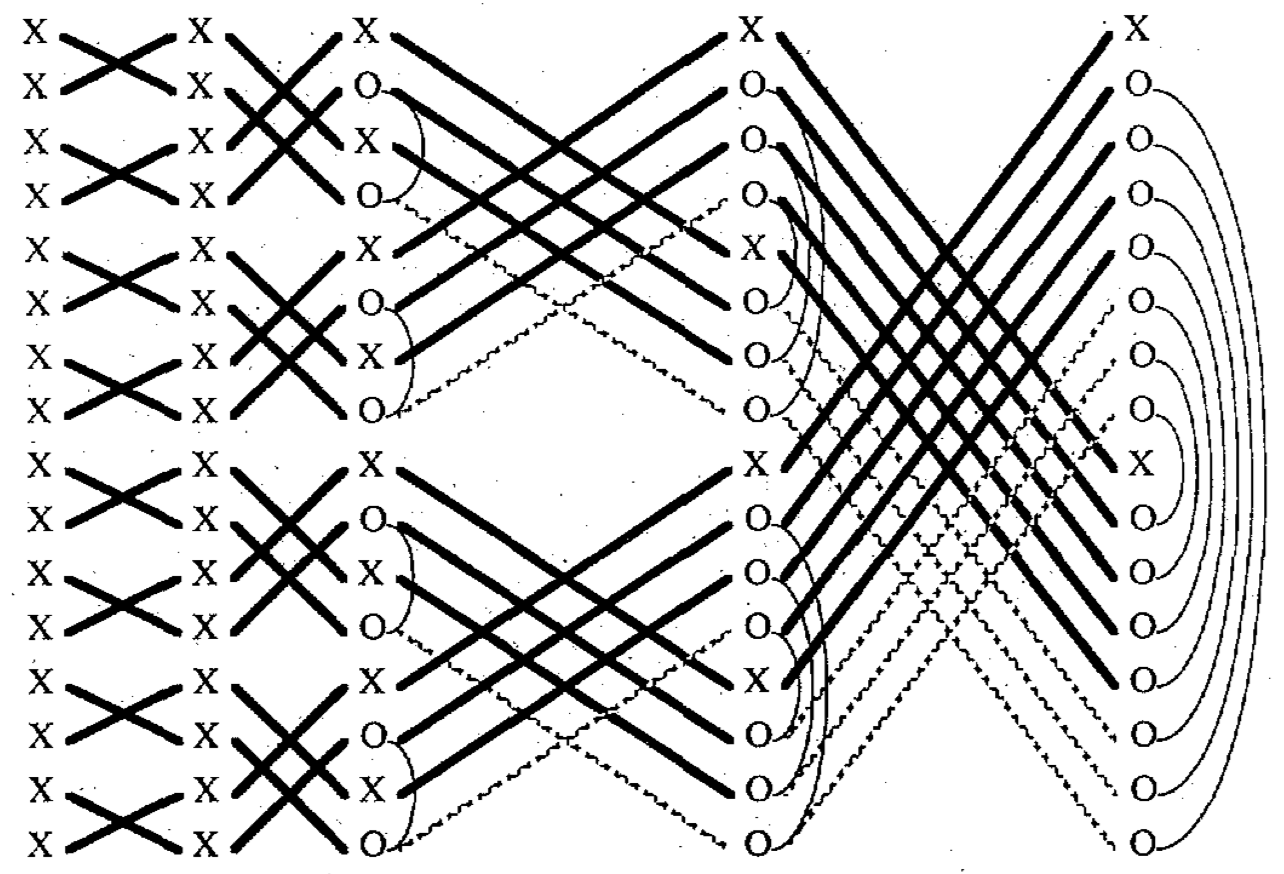
\includegraphics[scale=.45]{thesis/figures/rfft.png}
	\caption{An overview of the \gls{fft} in the case of real-valued inputs, where X indicates the real value and O represents the complex value. The figure shows the symmetric converted complex values \cite{sorensen_real-valued_1987}.}
	\label{an overview of the rfft}
\end{figure}

The data after \gls{rfft} processing contains two parts. One part is the \gls{dc} component, which can be regarded as the offset of the data and the other part is the Nyquist frequency component. In our data, when the dimension of a low resolution data obtained by double downsampling in time domain is \texttt{(256, 32)}, the dimension of the data in frequency domain will be in the shape of  \texttt{(129, 32)}, while the dimension of the low-resolution data obtained by quadruple downsampling is \texttt{(65, 16)}. Similarly, the shape of the high-resolution cube data will changed from \texttt{(512, 64)} to \texttt{(257, 64)}.

For the specific transform process, since \gls{fft} can only process time domain data of limited length, it is necessary to truncate the signal, that is, add a window, and each transform process is only performed within one window. The commonly used window functions include but not limit to the Hamming windows, Hanning windows, and blackman windows. For the two window functions built in TensorFlow, Hamming windows and Hanning windows, since the end of the Hamming window has a smaller main lobe in frequency domain which leads to a shaper range-Doppler map \cite{podder2014comparative}. Therefore, before performing \gls{rfft}, using the Hamming window function on the data cube during the \gls{rdp} is necessary.

After obtaining the windows of the range and Doppler effect axes respectively, we first apply the window on the range dimension and perform the \gls{rfft} operation. The dimension of the range will then change from 512 to 257 or from 256 to 129. The data after the \gls{rfft} operation on the range dimension is complex-valued. While applying the window on the velocity axis, it should be applied to the real and imaginary parts respectively. Since it is already complex-valued, only \gls{fft} is performed on the velocity dimension instead of \gls{rfft}. In addition, the \gls{fft} operation in TensorFlow only acts on the last dimension, so after finishing the transform on the range dimension, a transpose operation is required. Finally, since the range is between 0 and the maximum value, whereas the velocity can be in both positive and negative values, the data can be shifted so that the position where the velocity is zero centered, which is clear and convenient for the visualization. The pseudo code for this processing is shown in Algorithm \ref{pseudo code of rdp processing}.

\begin{algorithm}
    \caption{Pseudo code of \gls{rdp} processing}
    \label{pseudo code of rdp processing}
    \renewcommand{\algorithmicrequire}{\textbf{Input:}}
    \renewcommand{\algorithmicensure}{\textbf{Output:}}
    
    \begin{algorithmic}[1]
        \REQUIRE $Cube\ data\ in\ time\ domain\ as\ cube$
        \ENSURE $Range-Doppler\ map\ in\ frequency\ domain\ as\ rD$

        \STATE $range\_window\ =\ tf.signal.hamming\_window(tf.shape(cube)[2])$
        \STATE $doppler\_window\ =\ tf.signal.hamming\_window(tf.shape(cube)[1])$
        \STATE ~
        \STATE $cube\_windowed\ =\ cube\ *\ range\_window$
        \STATE $rfft\ =\ tf.signal.rfft(cube\_windowed)$
        \STATE $rfft\ =\ tf.transpose(rfft,\ perm=[0, 2, 1])$
        \STATE ~
        \STATE $re\_rfft\ =\ tf.math.real(rfft)\ *\ doppler\_window$
        \STATE $im\_rfft\ =\ tf.math.imag(rfft)\ *\ doppler\_window$
        \STATE $rfft\ =\ tf.complex(re\_rfft,\ im\_rfft)$
        \STATE $rD\ =\ tf.signal.fft(rfft)$
        \STATE ~
        \IF {$whether\_fftshift$}
            \STATE $rD\ =\ tf.signal.fftshift(rD, 2)$
        \ENDIF
        
    \end{algorithmic}
\end{algorithm}

\begin{spacing}{1.5}
\textbf{\large{\gls{irdp}}}
\end{spacing}

When the data needs to be converted from the frequency domain back to the time domain, the \gls{irdp} operation can be performed. The operation is the opposite of the above mentioned \gls{rdp} operation. First of all, make sure that the shape of each range-Doppler map is as the format of \texttt{(1, \#samples, \#chirps)}. The reason for the extra dimension at the first position is to emphasize the number of frames. The number of frames may be 4 as input, but in the output it goes to one frame. Next, use \gls{ifft} to process the velocity axis and calculate the window functions of the range dimension as well as the velocity dimension. Furthermore, since the range dimension has not yet recovered its original size, the dimension must be calculated additionally in the range window function. Then, after removing the window function in the real and imaginary parts and transposing the shape, \gls{irfft} and removing the range window function can be performed. The pseudo code is written in Algorithm \ref{pseudo code of irdp processing} as well.

\begin{algorithm}
    \caption{Pseudo code of \gls{irdp} processing}
    \label{pseudo code of irdp processing}
    \renewcommand{\algorithmicrequire}{\textbf{Input:}}
    \renewcommand{\algorithmicensure}{\textbf{Output:}}
    
    \begin{algorithmic}[1]
        \REQUIRE $Range-Doppler\ map\ in\ frequency\ domain\ as\ rD$
        \ENSURE $Cube\ data\ in\ time\ domain\ as\ cube$

        \STATE $num\_chirps\ =\ tf.shape(rD)[2]$
        \STATE $num\_samples\ =\ tf.shape(rD)[1]$
        \STATE $rD\ =\ tf.reshape(rD,\ (-1,\ num\_samples,\ num\_chirps))$
        \STATE ~
        \IF {$whether\_fftshift$}
            \STATE $rD\ =\ tf.signal.fftshift(rD, 2)$
        \ENDIF
        \STATE ~
        \STATE $rfft\ =\ tf.signal.ifft(rD)$
        \STATE $range\_window\ =\ tf.signal.hamming\_window((num\_samples-1)*2)$
        \STATE $doppler\_window\ =\ tf.signal.hamming\_window(num\_chirps)$
        \STATE ~
        \STATE $re\_rfft\ =\ tf.math.real(rfft)\ /\ doppler\_window$
        \STATE $im\_rfft\ =\ tf.math.imag(rfft)\ /\ doppler\_window$
        \STATE $rfft\ =\ tf.complex(re\_rfft,\ im\_rfft)$
        \STATE ~
        \STATE $rfft\ =\ tf.transpose(rfft,\ perm=[0, 2, 1])$
        \STATE $cube\_windowed\ =\ tf.signal.rfft(rfft)$
        \STATE $cube\ =\ cube\_windowed\ /\ range\_window$
        
    \end{algorithmic}
\end{algorithm}

\section{Pre- and post-processing of the model inputs and outputs} \label{pre- and post-processing of the model inputs and outputs}

According to the type and characteristics of the data, a more appropriate preprocessing will greatly promote the training of the model. Furthermore, the convolutional layer is common in the models. Currently, after processing by \gls{rdp}, the data is converted into complex value, whereas the convolutional layer can only be used to process the data in real value, so it needs to choose some preprocessing methods as well. In the pipeline, the following three processing steps are mainly used: the conversion from complex value to real value, that is, input data representation, the logarithm operation on the amplitude of the data, and the normalization of the data. The three processing steps contain different methods which can be combined in different ways.

\subsection{Input data representation} \label{separation types}
% real/imaginary separation
% incl. logarithm operation \& 10.0 power and cut-off to avoid the nan problem
In order to convert the range-Doppler map from complex value to real value, three different input data representations are introduced as real and imaginary representation, amplitude representation, as well as amplitude and phase representation. In addition, a very important preprocessing is about the dimensions. During the process of creating and loading \gls{tfrecord} files, mini batch dimension is introduced. Therefore, the current shape of the low-resolution data is \texttt{(batch, \#Frames, \#samples//sampling\_rate//2+1, \#chirps//sampling\_rate)}. According to the default setting of the convolutional layer in TensorFlow, the feature is always put in the last dimension, so the current data should be transposed, that is, transposed into \texttt{(batch, \#samples//sampling\_rate//2+1, \#chirps//sampling\_rate, \#Frames)}.

\begin{spacing}{1.5}
\textbf{\large{Real and imaginary representation}}
\end{spacing}

In this representation type, the real and imaginary parts of the input are taken out separately and concatenated. According to the above input size, the last dimension will be converted from \texttt{\#Frames} to \texttt{\#Frames*2}, that is, \texttt{(batch, \#samples//sampling\_rate//2+1, \#chirps//sampling\_rate, \#Frames*2)}. There are two options for the concating process. One option is to take features as the number of frames of the real part and features of the imaginary part separately and stack them directly on the last dimension, that is, \texttt{rrrriiii}, where \texttt{r} represents the real part and \texttt{i} indicates the imaginart part. Another is that separating each data and then stacking them, that is, \texttt{riririri}. After a quick experiment, we used a small model and part of the data and found that there's no big difference between these two, since the convolution is invariant to the permutation with respect to the channels. Therefore, in order to focus on more important improvements later and reduce the complexity of different combinations, the first option is used by default, that is, directly stacking the real and imaginary parts.

In this representation type, the number of kernels in the last convolutional layer in the models will be set as two, where the first dimension represents real part and the second dimension indicates imaginary part, so the final output of the model will be \texttt{(batch, \#samples//2+1, \#chirps, 2)}. While calculating the loss, this prediction is still used in this shape. Only for the visualization, the value will be considered to convert back. TensorFlow also provides a function for directly merging real and imaginary parts into a complex value.

\begin{spacing}{1.5}
\textbf{\large{Amplitude representation}}
\end{spacing}

According to the definition of range-Doppler map, there is an amplitude at the position corresponding to the range and velocity, which is a required parameter in the visualization and range-Doppler map upsampling. Therefore, a real value can be obtained by calculating the amplitude of each complex value, and the size of the input will be hence \texttt{(batch, \#samples//sampling\_rate//2+1, \#chirps//sampling\_rate, \#Frames)}.

In this case, the number of kernels in the last convolutional layer in all models will be set as 1, which represents the amplitude and the output shape would be \texttt{(batch, \#samples//2+1, \#chirps, 1)}. In the loss functions, only the difference between the amplitude can be calculated without any phase information. Meanwhile, this value is directly used while plotting the range-Doppler map, and the complex value or the signal in time domain cannot be restored.

\begin{spacing}{1.5}
\textbf{\large{Amplitude and phase representation}}
\end{spacing}

In order to retain as much information as possible, to facilitate the recovery of time domain signals and to add phase in the loss functions to supplement information, the amplitude and phase can also be concatenated. Its size will be \texttt{(batch, \#samples//sampling\_rate//2+1, \#chirps//sampling\_rate, \#Frames*2)}, and the last dimension will be concated as \texttt{aaaapppp}, where \texttt{a} represents amplitude and \texttt{p} represents phase. The output unit of the last convolutional layer in the models is 2, where the first one represents amplitude and the second dimension denotes phase.

\subsection{Logarithm operation} \label{logarithm operation}
% only in amplitude, with log10, with log2
Compared to the upsampling image or signal approaches in the state-of-art papers mentioned in section \ref{overview of the state of the art}, a significant difference is that the amplitude of our range-Doppler map in the indoor environment varies widely. As the detection range increases, the noise becomes greater and the \gls{snr} decreases. We hope that the model can also pay attention to areas with low signal power, so we need to reduce the dynamic range of the signal. One way is to perform logarithm operations on the data. For this part, there are currently two ways: no logarithm processing and logarithm processing with base 10.

\subsection{Normalization types} \label{normalization types}
% the normalisation of the input to be (-1,1) or (0,1), angle normalisation, and the global min/max/mean
In order to further reduce the dynamic range of the signal, the data can also be normalized. In addition to the amplitude, phase can also be normalized.

For amplitude normalization, there are two normalization ranges, namely (-1, 1) or (0, 1). First of all, we need to find the minimum, mean, and maximum values of the dataset. This part of the operation is performed when the \gls{tfrecord} files are reloaded but not yet converted into the mini batches. By mapping a loop in the dataset, the corresponding values can be iteratively found. The value searching and normalization operation will be performed on the training set, validation set, and test set separately, not the entire dataset. In addition, since in reality, the model can only get the low-resolution data as the input, while the high-resolution data is unknown to the model. Therefore, while calculating these values, it is based on the low-resolution data rather than the high-resolution data. Another reason is that although the data has been downsampled, the overall value range, the minimum, mean as well as maximum values and data distribution will not change much. It can be considered that the data range and distribution at low-resolution case are basically consistent with the high-resolution data.

If the range is going to be (-1,1), the normalization operation can be done by
\begin{equation}
    \centering
    \text{normalized data} = \frac{\text{data}}{\text{max}},
\end{equation}

where max means the maximum absolute value among the dataset and in case of the range (0,1), the equation should be written as
\begin{equation}
    \centering
    \text{normalized data} = \frac{\text{data - min}}{\text{max - min}}.
\end{equation}

In the case of real and imaginary representation, the normalization can be performed as 
\begin{equation}
    \centering
    \text{normalized data} = \frac{\text{data}}{\text{amplitude}}.
\end{equation}

Furthermore, since the phase is always in the range of (-\(\pi\), \(\pi\)), it can be divided by \(\pi\) to make its range fall into (-1, 1). In conclusion, the dataset can be preprocessing in these three types, and their combination can be summarized as Table \ref{combination of three different preprocessing types}.

\begin{table}
    \centering
    \caption{Combination of three different processing types, where \ding{56} represents the valid combination and - denotes no combination.}
    \label{combination of three different preprocessing types}
    \begin{tabular}{l|c|c|c}
        \hline
        \textbf{Combination} & Real/imaginary & Amplitude & Amplitude/phase\\
        \hline
        Logarithm operation & - & \ding{56} & \ding{56} \\
        \hline
        Amplitude normalization & \ding{56} & \ding{56} & \ding{56} \\
        \hline
        Angle normalization & - & - & \ding{56} \\
        \hline
    \end{tabular}
\end{table}

\section{Range-Doppler map visualization} \label{range-Doppler map visualization}
% plotting the rD map in logarithm, resolution calculation, maximum range and velocity, limit the value range of the bar.
In order to intuitively see the effect of upsampling, we can plot the range-Doppler map, which mainly includes three steps: restoring the processed part, calculating the required parameters, and drawing.

First of all, some postprocessing should be performed to reverse preprocessing, and then the parameters that need to be calculated include the amplitude of each point, range resolution, and velocity resolution. The formulas for calculating velocity and range resolution can be applied in the pipeline according to formulas \ref{velocity resolution equation} and \ref{range resolution equation}, and for the amplitude, it needs to be determined according to the input data representation. When the data is divided into real and imaginary parts, the square root of the sum of the squares should be calculated, and if it is separated by amplitude or amplitude and phase, the first value in the last dimension will be taken. In the visualization, the first range-Doppler map in the last batch of each epoch is used by default, that is, each epoch has one visualization plot. There are something also necessary to emphasize that while plotting low-resolution range-Doppler maps, the calculated resolution values must be changed according to the resampling rate. Meanwhile, since the data collected by radar device is in voltage unit, whereas the unit of range-Doppler map is in power, the above mentioned amplitude must be squared.

There are two additional settings in the range-Doppler visualization function. One is that the amplitude value can be drawn in linear scale or in dB unit. Since the data is postprocessed, the input of the visualization function is already in linear scale, but due to the large dynamic range in the data, in order to facilitate the observation of the low \gls{snr} part, the log scale is used by default, namely in dB unit. Another setting is that since the color bar in the range-Doppler map will produce different shades of colors as the amplitude in the range-Doppler map changes, in order to compare results clearly as well as according to the distribution of high-resolution data, the range in the color bar is set between -80 dB and 60 dB. When data exceeding this range exists, a warning will be displayed in logging. In the \gls{wandb} log, the corresponding low-resolution, predicted super-resolution, and high-resolution range-Doppler maps will be visualized together in this way.

\chapter{Models} \label{models}

In this chapter, we will build the models for range-Doppler map upsampling. According to the introduction in section \ref{overview of the state of the art}, there are mainly the following deep learning models, encoder-decoder architecture such as UNet architecture, Transformer model, \gls{cgan}, etc. Additionally, two layers are required in models, namely dimension processing layer and upsampling layer.

\section{Dimension processing layer} \label{dimension processing layer}
% padding or convolutional layer to make (129,32) to be (130, 32) or (128,32)
According to the \gls{rdp} introduced in section \ref{dataset loading} and the preprocessing types in section \ref{pre- and post-processing of the model inputs and outputs}, the input size of the model will be \texttt{(batch, \#samples//sampling\_rate//2+1, \#chirps//sampling\_rate, \#Frames or \#Frames*2)}. In order to explain the change of the shape easily and clearly, following will use the amplitude and phase representation type, batch size as 8, sampling rate as 2, the number of frames as 4 by default. In this combination, the shape of the low-resolution input will be \texttt{(8, 129, 32, 8)} and for high-resolution data as ground truth as \texttt{(8, 257, 64, 2)}. However, there is a problem with the current range dimension as an prime number. In the encoder-decoder architecture, it is difficult to choose a suitable stride for the current shape of the range axis because multiple times of the downsampling and upsampling layers will be performed. For the \gls{swin} Transformer, the current shape of range axis is also a troublesome size since the data needs to be split into multiple patches. Except the \gls{dp}-\gls{tf} Transformer model, since it calculates self-attention along the range and velocity axes separately, the problem of dimension does not need to be considered as well as our basic \gls{cnn} model, because it will not downsample the data.

There are three solutions for dimension processing layer. The first is that only in the case of \gls{dp}-\gls{tf} Transformer model and the basic \gls{cnn} model, it's possible to skip the additional dimension processing layer, and the model directly learns based on the input shape, but also ensure that there is no other downsampling process in the \gls{dp}-\gls{tf} Transformer model. In this case, since the model will perform an upsampling operation at the end, the dimension will become \texttt{(8, 258, 64, 2)}, so a cropping is required to select only the first 257 samples along the range axis.

Another option is that for models that need multiple downsampling layers such as in the encoder-decoder structure, it is more convenient when the range-Doppler map shape is in the power of 2, so the solution is to perform a convolutional layer along the range dimension, which uses a stride of 1 and the kernel size is set as \texttt{(2, 1)}, so that the input dimension of the model becomes \texttt{(8, 128, 32, 8)}. After passing through the model and subsequent upsampling layer, its dimension goes to \texttt{(8, 256, 64, 2)}. Therefore, there is always one less value in the range dimension. Then the transposed convolutional layer is needed, and also chosen stride as 1 and kernel size as \texttt{(2, 1)} to make its shape the same as ground truth.

However, while applying the convolutional layer according to the second option, the reduction in one dimension means that information may be lost. In order to alleviate this problem, the third solution is padding. By filling a row of 0 values along the range dimension, it will not lose input information and can become an even number, that is, the input becomes \texttt{(8, 130, 32, 8)}. Meanwhile, since it is not a power of 2, the downsampling layer can be performed only once in the model at most. In this case, after the final upsampling layer, the size of the output will be \texttt{(8, 260, 64, 2)}. There are extra \texttt{(2*sampling\_rate - 1)} samples in the range dimension, but since it was initially filled with 0, directly discarding this part will not cause information loss, that is, taking the values before the last \texttt{(2*sampling\_rate - 1)} dimension.

In summary, according to the input data representation, logarithm, normalization type as well as the dimension processing type, the preprocessing block can be combined with six forms as shown in Figure \ref{preprocessing_block}. The corresponding postprocessing module has six forms as well, illustrated in Figure \ref{postprocessing_block}. The green part in the preprocessing block is the input data that the model starts to process, while the red part in the postprocessing block is the output of the model for calculating the training loss with the ground truth.

\begin{figure}
	\centering
	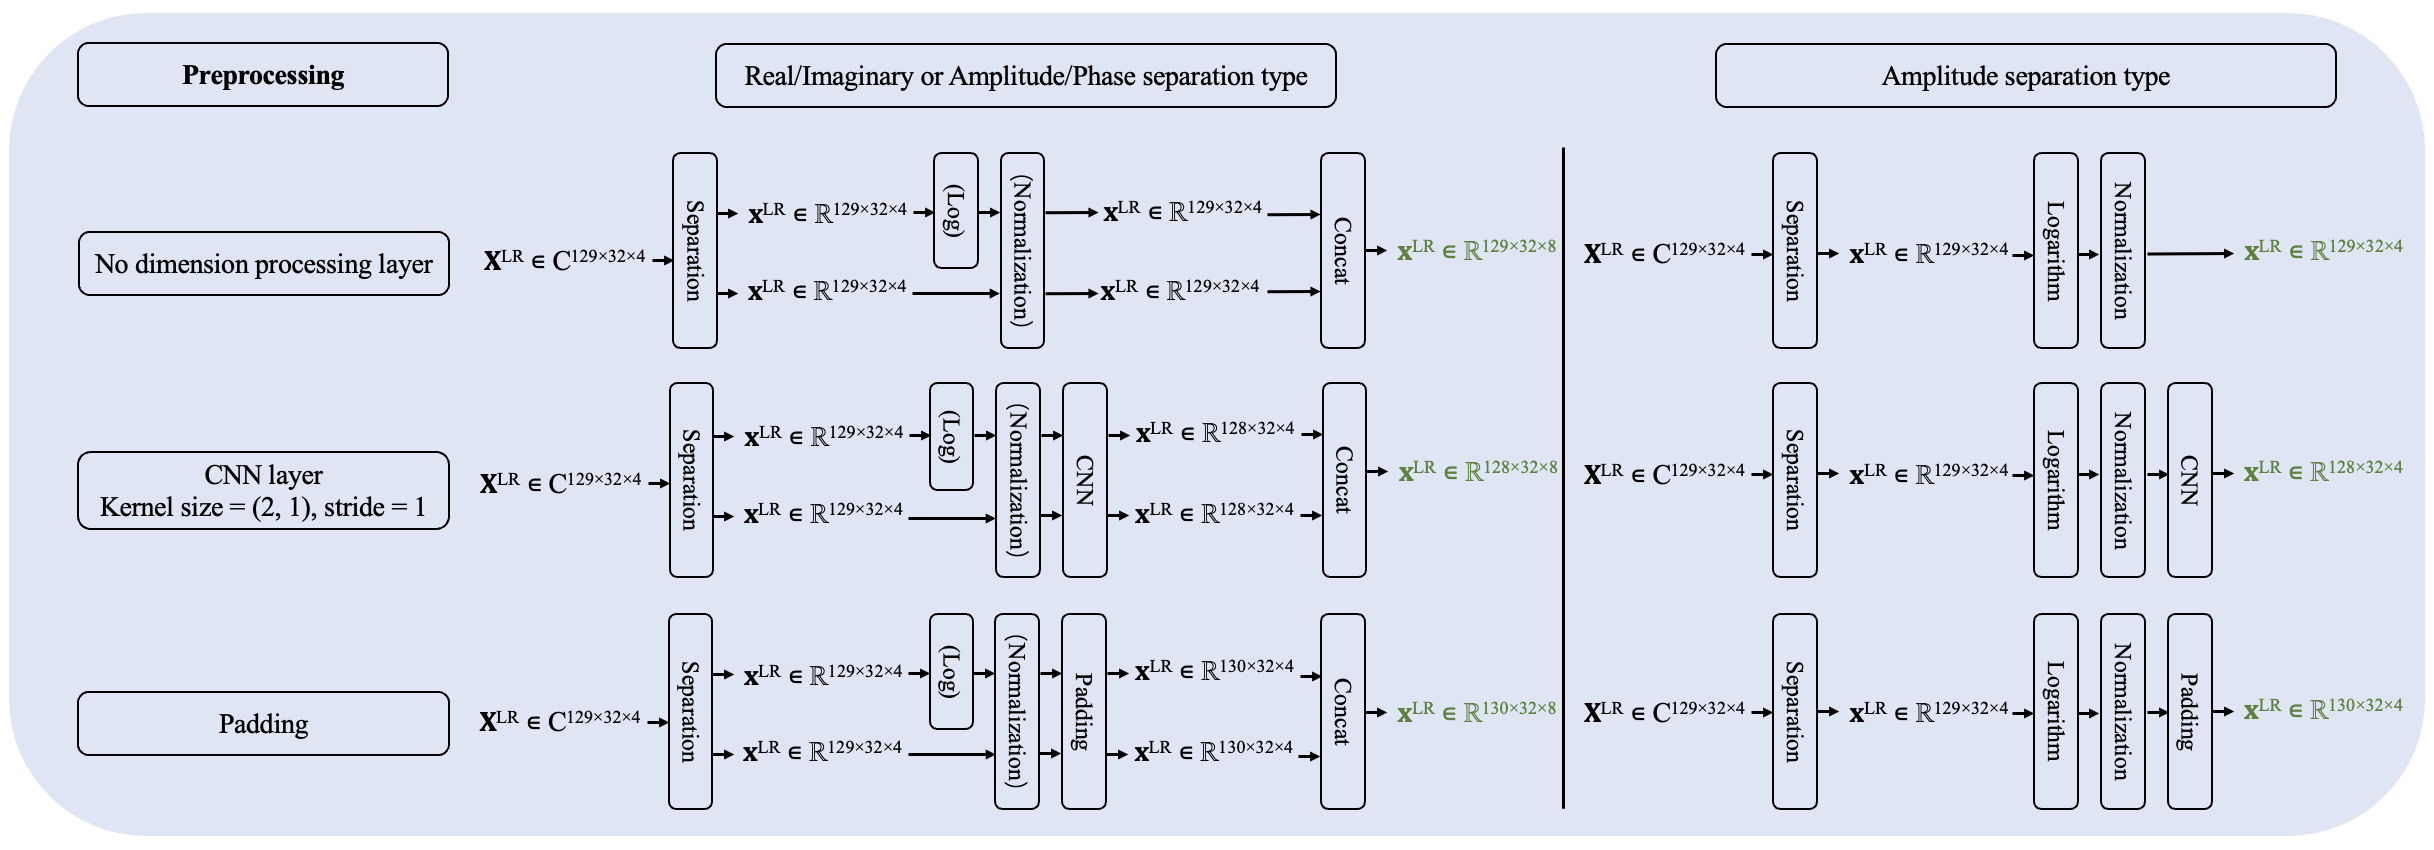
\includegraphics[scale=.45]{thesis/figures/preprocessing_block.png}
	\caption{Preprocessing block in the case of the number of frames as 4, where logarithm and normalization are not used in real and imaginary representation type and the green represents the model inputs.}
	\label{preprocessing_block}
\end{figure}

\begin{figure}
	\centering
	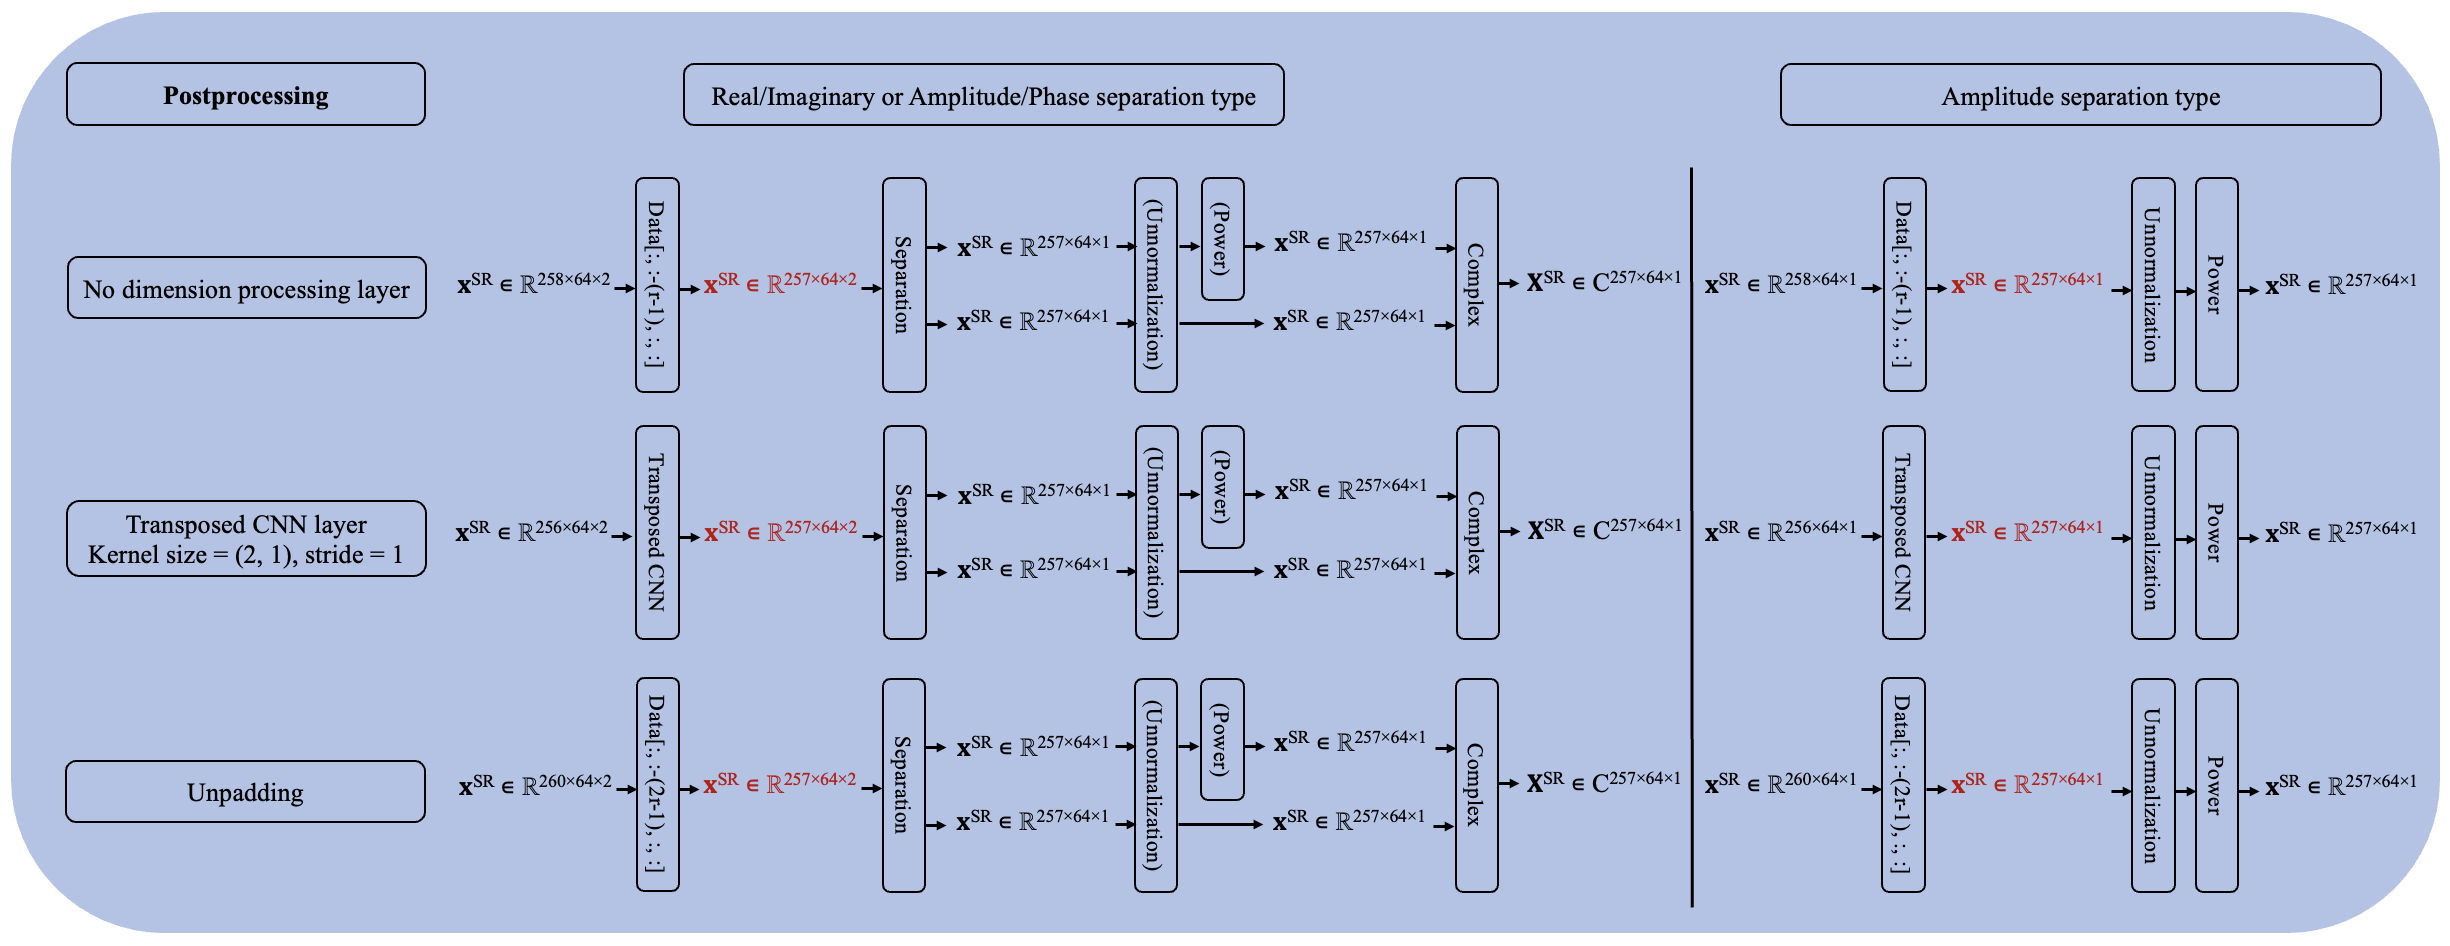
\includegraphics[scale=.42]{thesis/figures/postprocessing_block.png}
	\caption{Postprocessing block in the case of the number of frames as 4, where unnormalization and power of 10.0 are not used in real and imaginary representation type, the red represents the model outputs to calculate the training loss and r is the resample rate.}
	\label{postprocessing_block}
\end{figure}

\section{Upsampling layer} \label{upsampling layer}
% Transposed convolutional layer or Shuffle pixel
Before performing the upsampling layer, it's necessary to determine the times of upsampling layers required. Since the upsampling functions in TensorFlow or PyTorch usually doubles the resolution each time, the upsampling rate prefers to be a power of 2, so the times of upsampling operations in our case can be determined to be logarithmic sampling rate with the base as 2.

A common layer for upsampling is the transposed convolutional layer, whose operation is logically equivalent to the reverse convolutional layer as shown in Figure \ref{view of a transposed cnn layer}, but these two are not their respective inverse, that is, the transposed convolutional layer can not completely restore the range-Doppler map back to the original one before the convolutional layer. The shape relationship between the input and output of the transposed convolutional layer is
\begin{equation}
    \centering
    o = (i - 1) * s + k - 2 * p,
\end{equation}

where $s$ represents stride, $k$ is the kernel size, $p$ denotes the padding size, $i$ and $o$ are the shape of input and output, respectively.

\begin{figure}
	\centering
	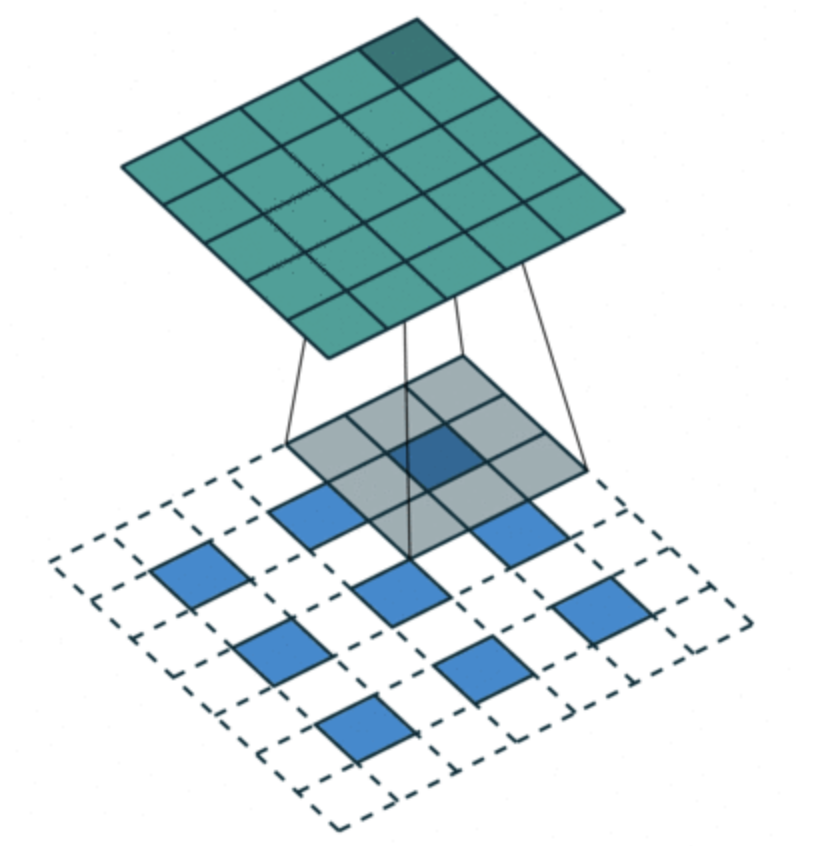
\includegraphics[scale=.45]{thesis/figures/transposed_cnn.png}
	\caption{View of the transposed convolutional layer in the case of the stride as 2, padding as 1 and kernel size as 3, where the blue is input and the green is output \cite{vdumoulin_vdumoulinconv_arithmetic_2025}.}
	\label{view of a transposed cnn layer}
\end{figure}

TensorFlow has a built-in transposed convolutional module. To facilitate upsampling, there are two options in the padding parameter, either valid or same. When same is selected, upsampling will be performed according to the stride value. Furthermore, each time the transposed convolutional layer is used, it will pass through the additional layer normalization and \gls{relu} activation layers as the other paper \cite{hinderer_blind_2022} did, which makes the training process more stable and converges faster as well as preventing the gradient explosion.

Another upsampling method is called pixel shuffle approach, also known as sub-pixel convolution or depth to space method, etc., proposed by Shi et al \cite{shi_real-time_2016}. As shown in Figure \ref{view of the pixel shuffle}, the principle is that the input data is processed by a series of hidden layers in the model, data of the shape \texttt{(N, C $\times$ r\textsuperscript{2}, H, W)} is obtained, where r denotes the resampling rate and all of the numbers are positive integers. Upsampling is achieved by splitting the size of \texttt{r\textsuperscript{2}} in depth and expanding its value into the dimensions of spaces, namely \texttt{H} and \texttt{W}.

There are two main benefits of pixel shuffle approach. Firstly, the pixel shuffle method does not require any other parameters, which can reduce the number of parameters and computational complexity compared to the transposed convolutional layer \cite{shi_is_nodate}. On the other hand, according to the paper from Odena, etc., one reason for the checkerboard effect is that the transposed convolutional layer causes overlapping, while the lack of overlapping in the method of pixel shuffle approach can mitigate this problem to a certain extent \cite{odena_deconvolution_2016}.

\begin{figure}
	\centering
	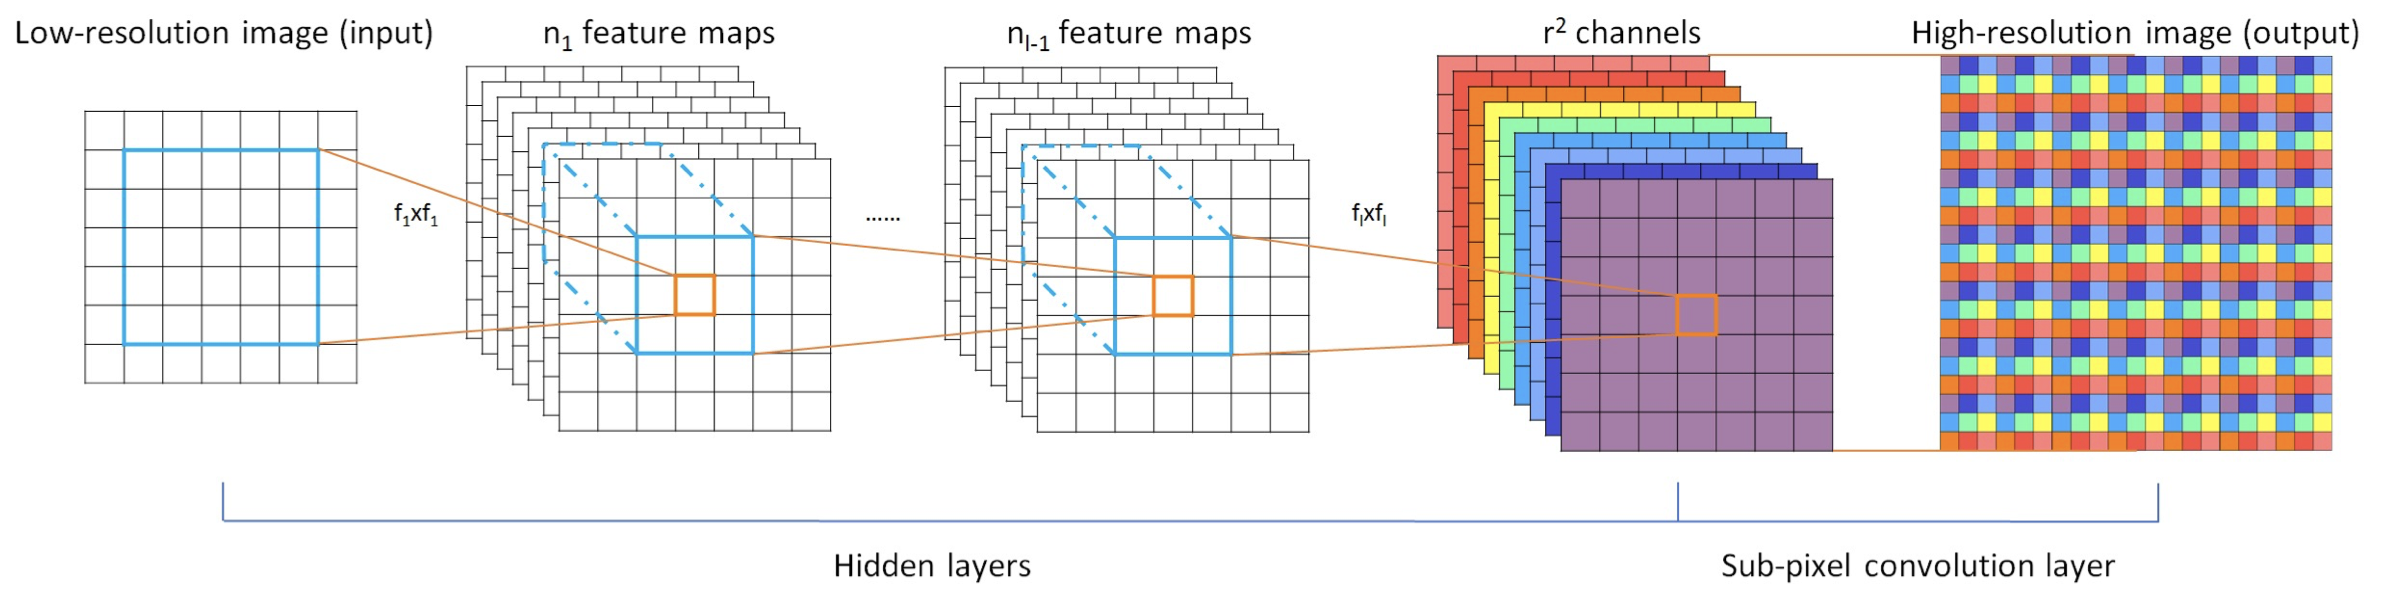
\includegraphics[scale=.35]{thesis/figures/pixelShuffle.png}
	\caption{View of the pixel shuffle approach, where r denotes the resample rate \cite{shi_real-time_2016}.}
	\label{view of the pixel shuffle}
\end{figure}

\section{Interpolation} \label{interpolation}
As a method that does not require any parameters and training process, the interpolation method can be used as a baseline in the range-Doppler upsampling task. Its principle is to interpolate a value in the middle according to the values of the surrounding points. Figure \ref{interpolation model} shows the interpolation model built in this thesis, which has two forms, Figure \ref{interpolation model left} and Figure \ref{interpolation model right}, according to the input data representation.

\begin{figure}
    \centering
    \hspace{-0.4cm}
    \begin{subfigure}{0.59\textwidth}
        \centering
        \adjustbox{height=12cm}{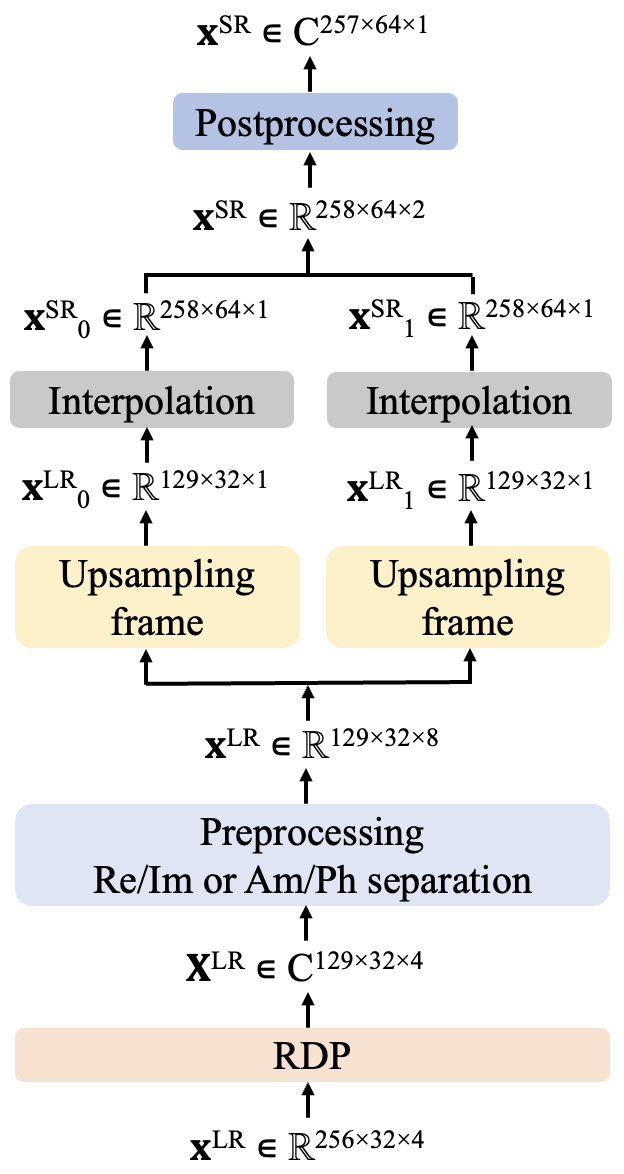
\includegraphics[scale=.25]{thesis/figures/interpolation_left.png}}
        \caption{Interpolation model with the real and imaginary or amplitude and phase representation types.}
        \label{interpolation model left}
    \end{subfigure}
    \begin{subfigure}{0.39\textwidth}
        \centering
        \adjustbox{height=12cm}{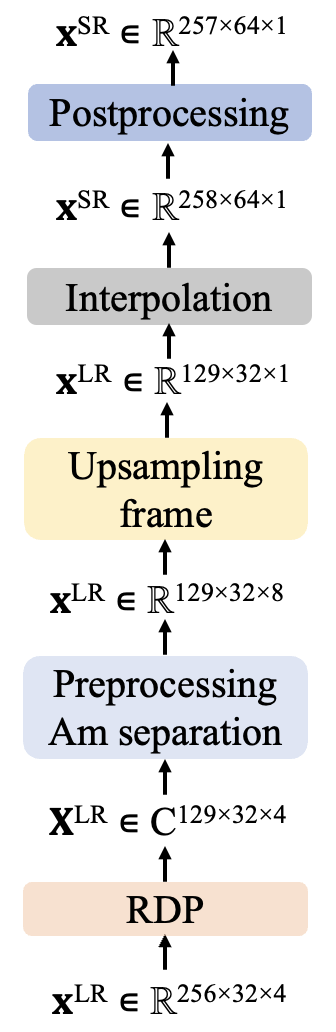
\includegraphics[scale=.25]{thesis/figures/interpolation_right.png}}
        \caption{Interpolation model with the amplitude representation type.}
        \label{interpolation model right}
    \end{subfigure}
    \caption{Interpolation models in terms of the representation types, in the case of the downsampling rate as 2 and the number of frames as 4.}
	\label{interpolation model}
\end{figure}

Assuming the same parameters as in section \ref{dimension processing layer} are used, that is, the batch size is set as 8, the data resampling rate is 2, and the number of frames is 4, the shape of the input is \texttt{(8, 129, 32, 8)} in the case of the real and imaginary or amplitude and phase representation types after preprocessing block. Since the interpolation method has no parameters and training process, it will directly process the low-resolution range-Doppler map which is going to be upsampled. According to the order of the number of frames in section \ref{dataset loading} and the input data representation mentioned in section \ref{pre- and post-processing of the model inputs and outputs}, the last dimension of the real part or the amplitude part $\text{x}^{\text{LR}}_0$ and the last dimension of the imaginary part or the phase part $\text{x}^{\text{LR}}_1$ are the data that need to be upsampled, so only these two frames are taken out.

For the interpolation process, TensorFlow provides many approaches. By default, bilinear interpolation is used in this model, as illustrated in Figure \ref{bilinear interpolation}, which is calculated based on the distance from the surrounding four points, namely
\begin{figure}
	\centering
	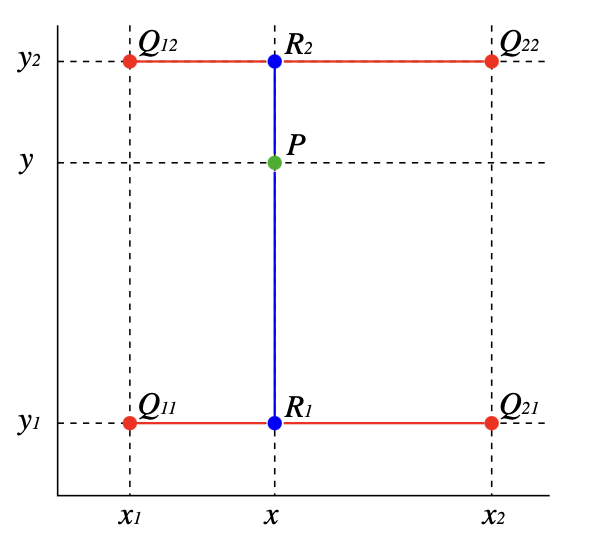
\includegraphics[scale=.7]{thesis/figures/bilinear.png}
	\caption{Bilinear interpolation, where $P$ is the interpolated point and $Q$s are the surrounding points \cite{noauthor_bilinear_2025}.}
	\label{bilinear interpolation}
\end{figure}

\begin{equation}
    \centering
    f(x, y) = \frac{1}{(x_2 - x_1)(y_2 - y_1)}
    \begin{bmatrix}
    x_2 - x & x - x_1
    \end{bmatrix}
    \begin{bmatrix}
    f(Q_{11}) & f(Q_{12}) \\
    f(Q_{21}) & f(Q_{22})
    \end{bmatrix}
    \begin{bmatrix}
    y_2 - y \\
    y - y_1
    \end{bmatrix},
\end{equation}

where $f(x, y)$ is the interpolation value at the point $(x, y)$. Furthermore, the default upsampling rate is 2 each time, so the sampling rate should be a power of 2. The model will be postprocessed according to the value of the resampling rate and as mentioned in section \ref{dimension processing layer} to make it the same size as the ground truth after stacking along the last dimension.

\section{CNN model} \label{cnn model}
Compared with the bilinear interpolation model, the most common model for image processing is the \glsfirst{cnn}. We introduced a relatively basic \gls{cnn} model, which does not downsample the data and performs the upsampling operation after one specified convolutional layer. The overview of the \gls{cnn} model is shown in Figure \ref{cnn model structure}.

\begin{figure}
	\centering
	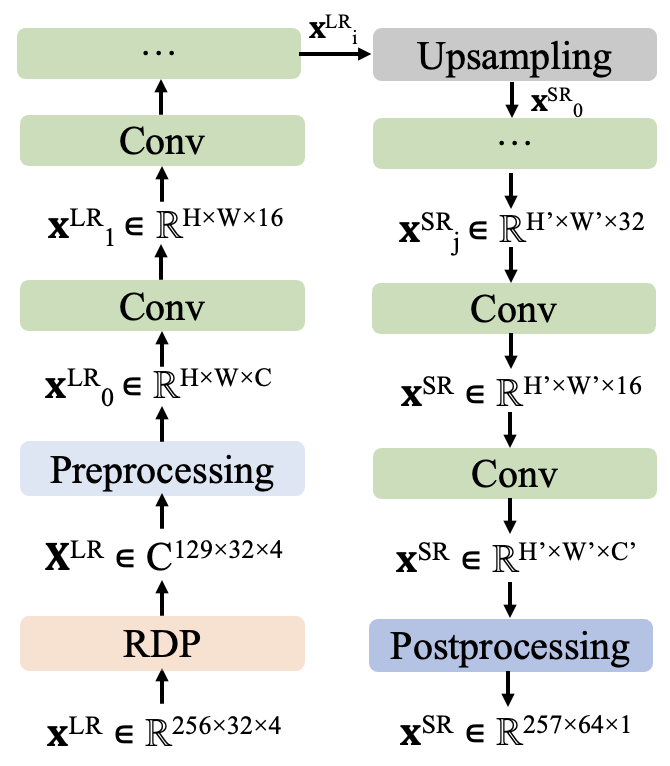
\includegraphics[scale=.63]{thesis/figures/cnn_simple.png}
	\caption{CNN model, where the channel, height and width are depending on the processing methods.}
	\label{cnn model structure}
\end{figure}

As shown, since the preprocessing is a combination of representation, dimension processing, logarithm and normalization types, the height \texttt{H} and width \texttt{W} depend on the selected dimension processing type, while the channel \texttt{C} and \texttt{C'} depend on the input data representation. The value of \texttt{C} can be 4 or 8, and then enters the convolutional layers. In this model, two parameters are set to facilitate the change of model scale, namely the neuron list and upsampling layer index. The neuron list represents a list of the channel values in the case of stride as 1, and the upsampling layer index indicates the position of the convolutional layer after which the upsampling layer is performed. Similarly, \texttt{H'} and \texttt{W'} are the sizes of the range-Doppler map after upsampling, which are also up to the dimension processing type, and are then converted into the same shape as the ground truth while postprocessing. The process can be written as

\begin{equation}
    \centering
    \text{x}^{\text{LR}}_i = \text{Conv2D}^{i}(\text{x}^{\text{LR}}_0),
\end{equation}

where $i$ is the upsampling layer index with the upsampling operation

\begin{equation}
    \centering
    \text{x}^{\text{SR}}_0 = \text{Upsampling}(\text{x}^{\text{LR}}_i),
\end{equation}

then the final super-resolution data after $j$ times convolutional layers is

\begin{equation}
    \centering
    \text{x}^{\text{SR}} = \text{Conv2D}(\text{Conv2D}^{j}(\text{x}^{\text{SR}}_0)).
\end{equation}

\begin{figure}[t]
	\centering
	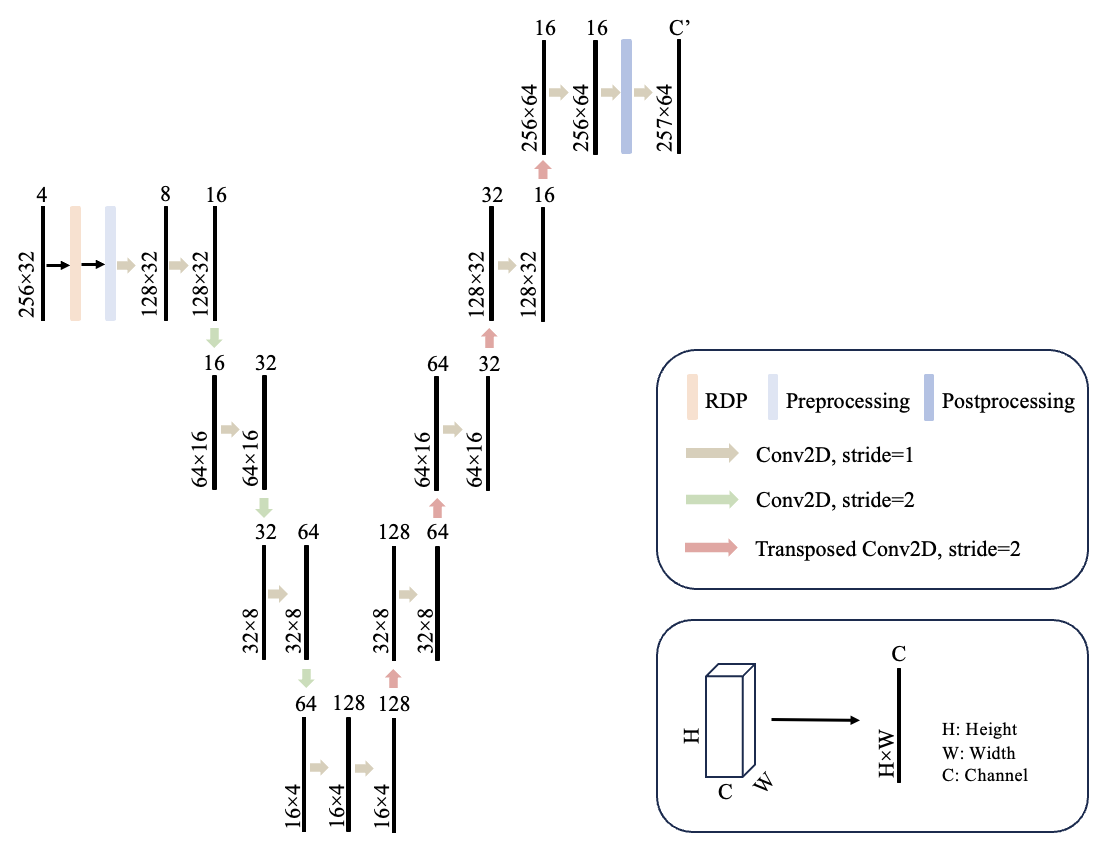
\includegraphics[scale=.8]{thesis/figures/unet_model.png}
	\caption{UNet model}
	\label{unet model}
\end{figure}

\section{UNet architecture} \label{u-net architecture}
As mentioned in section \ref{overview of the state of the art}, the encoder-decoder structure is very common for the upsampling task in deep learning. During the encoder process, the model will do the downsampling operations and learn important features from the data, and then perform multiple upsampling layers based on the learned information. The most common model is the UNet model, so we built it based on the convolutional layers with the stride as 2. Compared with the \gls{cnn} model in section \ref{cnn model}, the downsampling process may cause information loss. Inspired by the paper \cite{prabhakara_high_2023} from Akarsh et al., by adding residual connections between the encoder and decoder parts, the information loss problem is alleviated. Therefore, in this section, there will be two parts, namely basic UNet model and UNet concat model.

\subsection{UNet model} \label{UNet model subsection}
The overview of the UNet model is illustrated in Figure \ref{unet model}. Since there are multiple downsampling operations in the UNet model and the default downsampling rate is 2, the data size in height and width should be the power of 2. Therefore, the dimension processing layer is determined as the convolutional layer approach in most cases. Otherwise, only once downsampling can be done if using padding. Meanwhile, due to the representation type, the channel would be either 4 or 8, and while passing through the first convolutional layer, this dimension is uniformly converted to 8.

In the UNet model, four times downsamplings are performed by default, and different numbers of upsampling layers are performed according to the resampling rate. When the resampling rate is 2, five times upsampling are performed. Before each upsampling layer, a convolutional layer with a stride of 1 is performed, and the number of channels is meanwhile modified. The upsampling operation uses the transposed convolutional layer by default. In postprocessing part, the corresponding unit parameters are set according to the data representation type.

\subsection{UNet concat model} \label{UNet concat model subsection}
As mentioned above, to mitigate the information loss during downsamping operations, in UNet concat model the upsampling data will be concatenated with the downsampled data, as shown in Figure \ref{unet_concat model}. 

\begin{figure}
	\centering
	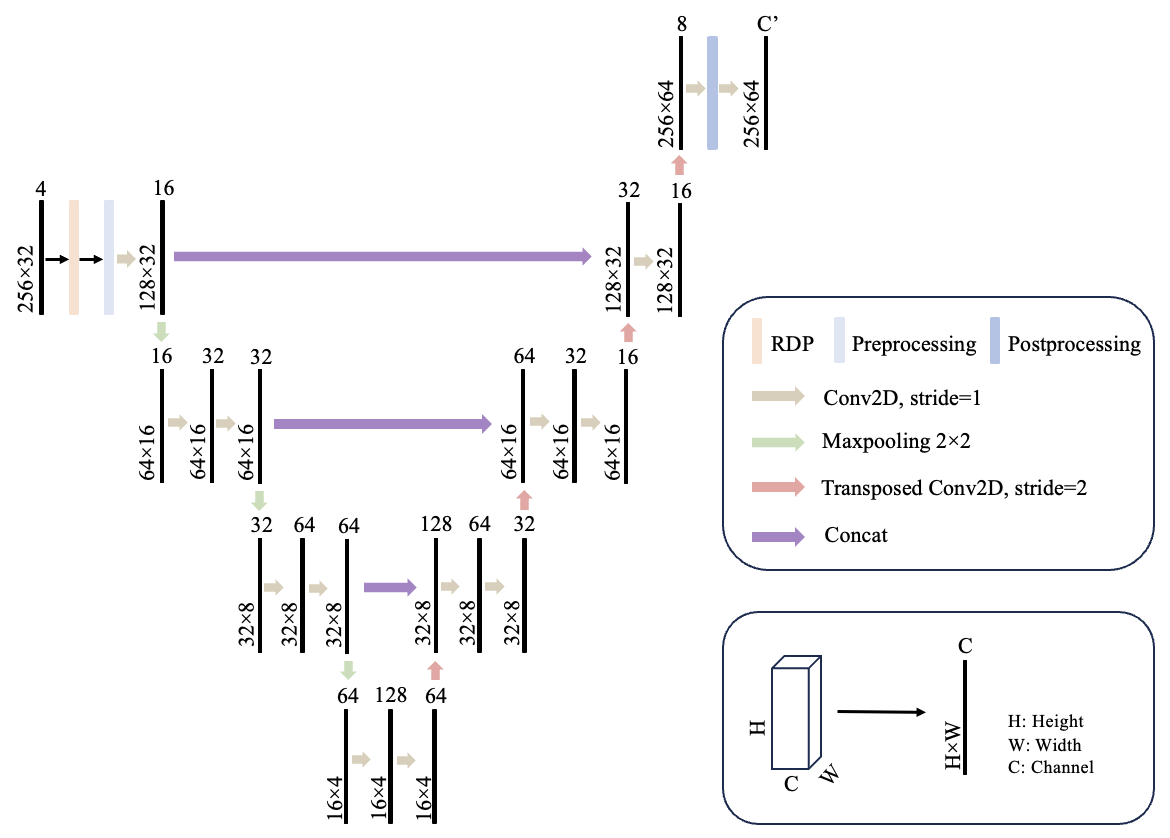
\includegraphics[scale=.75]{thesis/figures/unet_concat.png}
	\caption{UNet concat model}
	\label{unet_concat model}
\end{figure}

Compared with the UNet model in section \ref{UNet model subsection}, the UNet concat model has the following four main differences. First, the encoder part passes through two convolutional layers with a stride of 1 instead of just one layer. Moreover, in the decoder part, the UNet model only passes through the convolutional layer once to reduce the channel before the upsampling layer, while UNet concat model passes through two convolutional layers and reduces the channel dimension twice. The UNet model uses a convolutional layer with a stride of 2 for downsampling, while UNet concat model uses a 2$\times$2 maxpooling layer. In addition, during each upsampling process, the data is concatenated with the corresponding downsampled data of the same size along the channel dimension.

\section{DP-TF Transformer architecture} \label{dp-tf transformer architecture}
As mentioned in section \ref{overview of the state of the art}, Transformer is a state-of-the-art model in the task of data upsampling. It uses the self-attention mechanism to learn the similarities and relationships between different blocks. In the range-Doppler map, the objects have a certain correlation in the dimension of the range and velocity related to the radar. Furthermore, the consecutive motion can also bring some additional motion information as well. In this model, it will mainly focus on the division along the two dimensions of range and velocity.

Figure \ref{dp-tf_transformer_architecture} shows the overall structure of this model. Compared with the models mentioned previously, it mainly has three different blocks: feature extractor, feature Transformer, and reconstruction. According to \cite{hinderer_blind_2022}, feature extractor is equivalent as an encoder, but since additional downsampling may cause information loss, the stride of the convolutional layer will be set as 1 in the featur extractor. The reconstruction is equivalent as the decoder, and the additional upsampling is performed according to the resample rate.

\begin{figure}
	\centering
	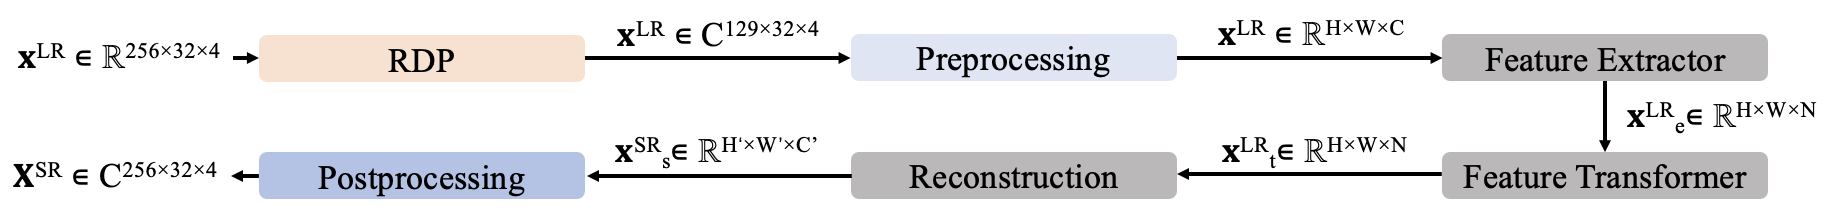
\includegraphics[scale=.5]{thesis/figures/dp-tf_transformer_architecture.png}
	\caption{DP-TF Transformer architecture, adapted from \cite{hinderer_blind_2022}.}
	\label{dp-tf_transformer_architecture}
\end{figure}

\begin{spacing}{1.5}
\textbf{\large{Feature Extractor}}
\end{spacing}

The feature extractor mainly includes two steps. The first step will perform a separable convolutional layer and a \gls{ln} to obtain an intermediate feature extractor representation $\mathrm{x^{LR}_{e1}}$ expressed as

\begin{equation}
    \centering
    \mathrm{x^{LR}_{e1} = LN(SeparableConv2D(x^{LR}))},
    \label{first separable conv2D equation in feature extractor}
\end{equation}

where $\mathrm{x^{LR}_{e1} \in \mathbb{R}^{H\times W\times N}}$ and H, W and N represent the height, width and channel size, respectively. In the second step, a SeparableConv2D layer and a \gls{ln} are also performed, where SeparableConv2D layer still sets stride as 1 and does not perform downsampling in our case. In addition, a \gls{relu} activation function layer will be used, written as

\begin{equation}
    \centering
    \mathrm{x^{LR}_{e2} = ReLU(LN(SeparableConv2D(x^{LR}_{e1})))},
    \label{second conv block after first conv in feature extractor}
\end{equation}

where $\mathrm{x^{LR}_{e2} \in \mathbb{R}^{H\times W\times N}}$ still. According to the paper, another convolutional layer is used. Although the downsampling operation is not performed in our case, we can still keep it. The output of the feature extractor can be written as

\begin{equation}
    \centering
    \mathrm{x^{LR}_{e} = LN(Conv2D(x^{LR}_{e2}))}.
    \label{third equation in feature extractor}
\end{equation}

\begin{spacing}{1.5}
\textbf{\large{Feature Transformer}}
\end{spacing}

The feature Transformer mainly includes three hierarchies, as shown in Figures \ref{feature_transformer_block}, \ref{dp_transformer_block}, and \ref{transformer_block}. Figure \ref{feature_transformer_block} shows the overall structure of the feature Transformer, Figure \ref{dp_transformer_block} shows the structure of the \gls{dp}-\gls{tf} Transformer block and the way to do the data segmentation, and Figure \ref{transformer_block} shows the structure of the \gls{te}.

\begin{figure}
	\centering
	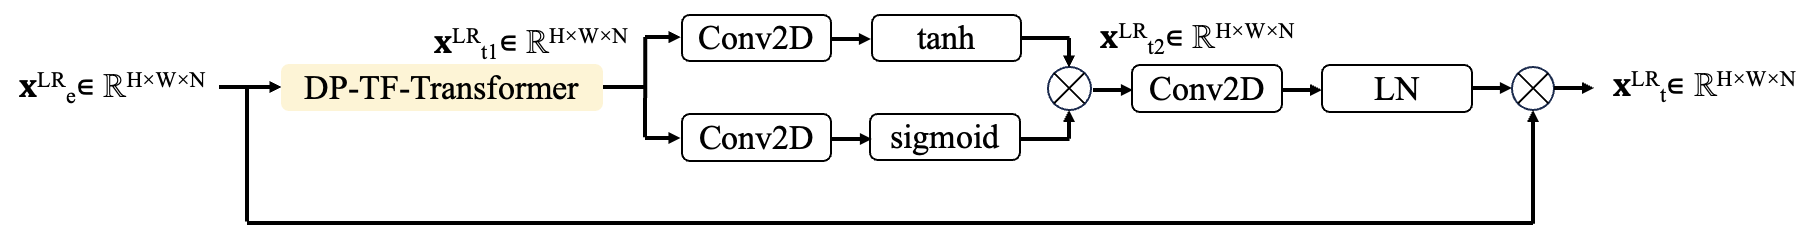
\includegraphics[scale=.48]{thesis/figures/feature_transformer_block.png}
	\caption{Feature Transformer block, adapted from \cite{hinderer_blind_2022}.}
	\label{feature_transformer_block}
\end{figure}

\begin{figure}
	\centering
	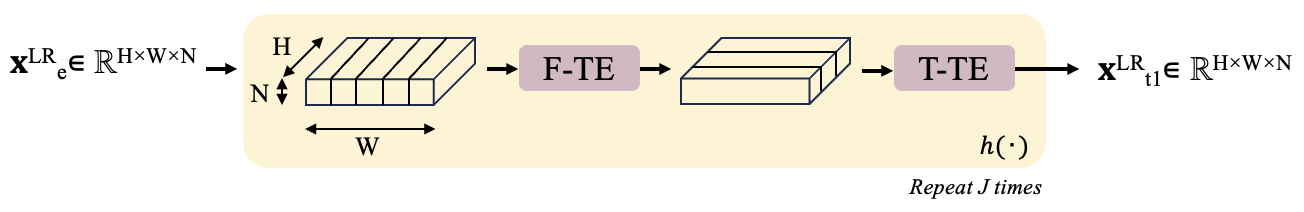
\includegraphics[scale=.66]{thesis/figures/dp_transformer_block.png}
	\caption{DP-TF Transformer block, adapted from \cite{hinderer_blind_2022}.}
	\label{dp_transformer_block}
\end{figure}

\begin{figure}
	\centering
	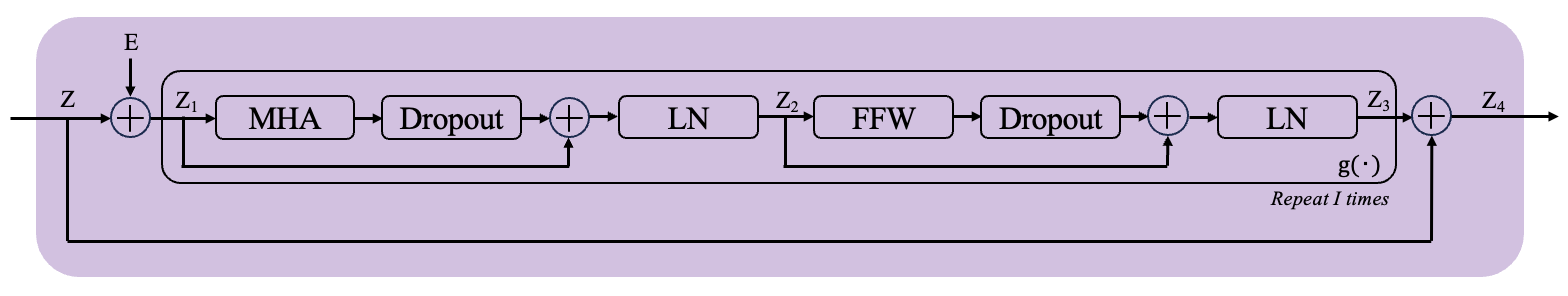
\includegraphics[scale=.55]{thesis/figures/transformer_block.png}
	\caption{TE block, adapted from \cite{hinderer_blind_2022}.}
	\label{transformer_block}
\end{figure}

In the first hierarchy of the feature Transformer, the data will be firstly operated by the \gls{dp}-\gls{tf} Transformer block. Subsequently, the output passes through the dual path which can be seen as a gating mechanism. Each path includes a convolutional layer and an activation function. The activation function as tanh keeps the main content into (-1, 1) while the other activation function uses sigmoid that leads the output into (0, 1). Then the two values are multiplied elementwise which is beneficial for remaining the useful information and discarding the feature with lower importance, namely
\begin{equation}
    \centering
    \mathrm{x^{LR}_{t2} = tanh(Conv2D(x^{LR}_{t1})) \circ sigmoid(Conv2D(x^{LR}_{t1}))}.
    \label{first equation in feature transformer}
\end{equation}

Furthermore, an additional convolutional layer and a layer normalization will be performed as well as a residual path, written as
\begin{equation}
    \centering
    \mathrm{x^{LR}_{t} = x^{LR}_{e} \circ LN(Conv2D(x^{LR}_{t2}))}.
    \label{second equation in feature transformer}
\end{equation}

In the second hierarchy, that is, in the \gls{dp}-\gls{tf} Transformer block, the data are divided along the range and velocity axes and each division has a \gls{te} block respectively, described as
\begin{equation}
    \centering
    \mathrm{x^{LR}_{t1}} = h^{j}\mathrm{(x^{LR}_{e})},
\end{equation}

where $h^{j}(\cdot)$ denotes $J$ times \gls{dp}-\gls{tf} Transformer block applications. Within the \gls{te} block, a sinusoidal positional encodings will be firstly added to the input as the representation of the order of the inputs, namely
\begin{equation}
    \centering
    \mathrm{Z_1 = Z + E},
\end{equation}

then a module $g(\cdot)$ as shown in Figure \ref{transformer_block} will be performed $I$ times on $\mathrm{Z_1}$ with a residual path with Z, written as
\begin{equation}
    \centering
    \mathrm{Z_4} = g^{I}\mathrm{(Z_1) + Z},
\end{equation}

where within this module, a multi-head attention block and a dropout layer will be performed on $\mathrm{Z_1}$, a residual path exists before the layer normalization, resulting in $\mathrm{Z_2}$
\begin{equation}
    \centering
    \mathrm{Z_2 = LN(Z_1 + Dropout(MHA(Z_1)))}.
\end{equation}

Moreover, another similar part will be performed, replace the MHA with a point-wise \gls{ffw} network, resulting in $\mathrm{Z_3}$
\begin{equation}
    \centering
    \mathrm{Z_3 = LN(Z_2 + Dropout(FFW(Z_2)))},
\end{equation}

where \gls{ffw} block contains two dense layers and a \gls{relu} activation function, that is,
\begin{equation}
    \centering
    \mathrm{Z'_2 = Dense(ReLU(Dense(Z_2)))},
    \label{ffw equation}
\end{equation}

\begin{spacing}{1.5}
\textbf{\large{Reconstruction}}
\end{spacing}

In the super-resolution data reconstruction, an upsampling layer will be performed firstly. If the transposed convolutional layer is used, it will combine with a layer normalization and a \gls{relu} activation function, namely
\begin{equation}
    \centering
    \mathrm{x^{SR}_{s1} = ReLU(LN(Conv2DTranspose(x^{LR}_t)))}.
    \label{separator1 equation}
\end{equation}

According to the input data representation, the unit of the last convolutional layer could be determined as either 1 or 2 with the linear activation, written as
\begin{equation}
    \centering
    \mathrm{x^{SR}_s = Conv2D(x^{SR}_{s1})}.
    \label{separator2 equation}
\end{equation}

\section{SwinIR Transformer architecture} \label{swinir transformer architecture}
According to \cite{liang_swinir_2021} mentioned in section \ref{overview of the state of the art}, in addition to dividing the data along the two dimensions of range and velocity, it can also be divided into multiple quadratic range velocity patches. The structure is shown in Figure \ref{swinir_architecture}, which mainly includes three parts: shallow feature extraction, deep feature extraction, and super-resolution image reconstruction.

\begin{figure}
	\centering
	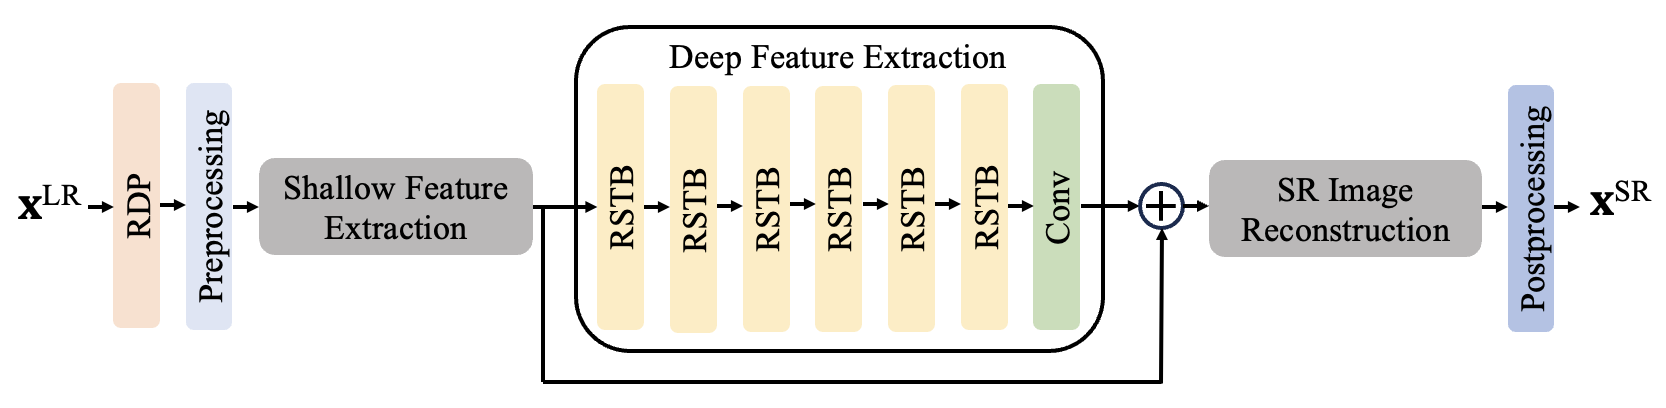
\includegraphics[scale=.53]{thesis/figures/swinir_architecture.png}
	\caption{SwinIR architecture, adapted from \cite{liang_swinir_2021}.}
	\label{swinir_architecture}
\end{figure}

In the paper, the \gls{swin} Transformer is used in the \gls{swinir} architecture, since we still have a \gls{dp}-\gls{tf} Transformer block, they can be combined as two models, namely SwinIR+Swin model and SwinIR+DP model.

\subsection{SwinIR+Swin model}

\begin{spacing}{1.5}
\textbf{\large{Shallow feature extraction}}
\end{spacing}

In the paper, the shallow feature extraction is seen as an encoder, which downsamples the data once. In order to mitigate the impact of information loss, a convolutional layer is still performed here but the stride is determined as 1, then the data size remains unchanged while only the channel is increased, namely
\begin{equation}
    \centering
    \mathrm{x^{LR}_s = Conv2D(x^{LR})}.
    \label{conv2D in shallow feature extraction equation}
\end{equation}

\begin{spacing}{1.5}
\textbf{\large{Deep feature extraction}}
\end{spacing}

In deep feature extraction, a dropout layer is performed first, then multiple \gls{rstb} and a convolutional layer are included, and the output of the deep feature extraction block is combined with the result of shallow feature extraction using the residual path, that is,
\begin{equation}
    \centering
    \text{x}^{\text{LR}}_\text{d} = \text{Conv2D}(\text{RSTB}^{J}(\text{Dropout}(\text{x}^{\text{LR}}_\text{s}))) + \text{x}^{\text{LR}}_\text{s},
    \label{first equation in deep feature extraction}
\end{equation}

where $J$ denotes the times of the \gls{rstb} applications. Figure \ref{rstb_block} illustrates the structure of the \gls{rstb}, where it contains multiple \gls{stl} blocks and a convolutional layer as well as the residual path, namely
\begin{equation}
    \centering
    \mathrm{{Z}_{R1}} = \text{Conv2D}(\text{STL}^{I}(\mathrm{Z_{R}})) + \mathrm{Z_{R}},
\end{equation}

where $I$ represents the times of the \gls{stl} applications. There are two parts inside the \gls{stl} block, one part includes a layer normalization, a \gls{msa} block as well as the residual part, described as
\begin{equation}
    \centering
    \mathrm{Z_{S1} = MSA(LN(Z_{S})) + Z_{S}},
\end{equation}

while another part contains a layer normalization, a \gls{mlp} and the residual path, namely
\begin{equation}
    \centering
    \mathrm{Z_{S2} = MLP(LN(Z_{S1})) + Z_{S1}}.
\end{equation}

In the \gls{mlp} block, five steps are carried out in sequence, namely dense layer, GeLU activation function, dropout layer, dense layer with linear activation function and dropout layer, denoted as
\begin{equation}
    \centering
    \mathrm{Z_{M1} = Dropout(GeLU(Dense(Z_{M})))},
    \label{mlp equation1}
\end{equation}

\begin{equation}
    \centering
    \mathrm{Z_{M2} = Dropout(Dense(Z_{M1}))}.
\end{equation}

\begin{figure}
    \centering
    \hspace{-0.4cm}
    \begin{subfigure}{0.49\textwidth}
        \centering
        \adjustbox{height=3.9cm}{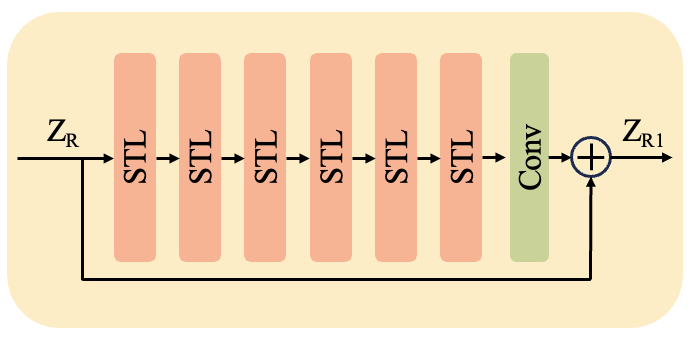
\includegraphics[scale=.24]{thesis/figures/rstb_block.png}}
        \caption{Structure of the \gls{rstb} block}
        \label{rstb_block}
    \end{subfigure}
    \begin{subfigure}{0.49\textwidth}
        \centering
        \adjustbox{height=3.75cm}{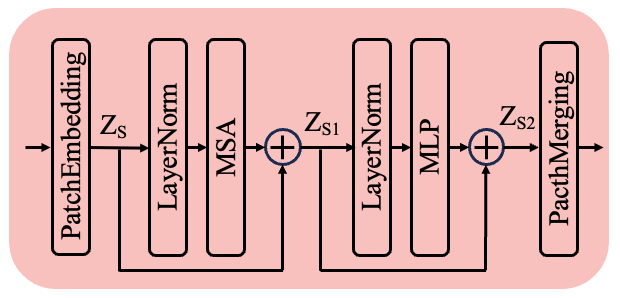
\includegraphics[scale=.24]{thesis/figures/stl_block.png}}
        \caption{Structure of the \gls{stl} block}
        \label{stl_block}
    \end{subfigure}
    \caption{The structure of \gls{rstb} and \gls{stl} blocks, adapted from \cite{liang_swinir_2021}.}
	\label{structure of the rstb and stl blocks}
\end{figure}

\begin{spacing}{1.5}
\textbf{\large{SR Image Reconstruction}}
\end{spacing}

The SR image reconstruction block includes three parts: the upsampling part as well as convolutional part before and after upsampling. There is a convolutional layer with the LeakyReLU activation function before the upsampling part, that is,
\begin{equation}
    \centering
    \mathrm{x^{LR}_{r} = LeakyReLU(Conv2D(x^{LR}_{d}))}.
\end{equation}

In the next step, the upsampling part is same as the reconstruction part in the section \ref{dp-tf transformer architecture}, namely the equation \ref{separator1 equation} and \ref{separator2 equation} resulting in $\mathrm{x^{SR}_{r1}}$ if using the transposed convolutional layer. After the upsampling part, another convolutional layer with the linear activation function is performed to make sure that the channel dimension of the output is according to the input data representation, namely the unit as either 1 or 2, written as
\begin{equation}
    \centering
    \mathrm{x^{SR}_r = Conv2D(x^{SR}_{r1})}.
\end{equation}

\subsection{SwinIR+DP model}
Combining with \gls{dp}-\gls{tf} Transformer block, the difference between SwinIR+Swin model is the \gls{stl} block. The structure of the \gls{stl} block as shown in Figure \ref{stl_block} can be replaced by the \gls{dp}-\gls{tf} Transformer block which is illustrated in Figure \ref{dp_transformer_block}.

\section{Comparison between the architectures} \label{comparison between the architecture}
According to all the models mentioned above, the differences between most models are relatively clear. For example, there is no downsampling process in the \gls{cnn} model. The difference between UNet and UNet concat models is mainly whether to combine the data of the encoder part with the corresponding decoder part. However, for the \gls{dp}-\gls{tf} Transformer model, the SwinIR+DP and SwinIR+Swin models, the data division is the main difference, but there are still some other small differences. Therefore, this section will focus on two parts, one is the difference between the \gls{dp}-\gls{tf} Transformer and \gls{swinir} architectures, and the other is the difference between the \gls{dp}-\gls{tf} and \gls{stl} Transformer blocks. The evaluation of this section will shown in the appendix.

\subsection{Differences between DP-TF and SwinIR Transformer architectures}
The main structures of the two architectures are very similar, both of which contain three parts: encoder, deep feature extraction, and decoder, so the differences will be listed in this order.

\begin{spacing}{1.5}
\textbf{\large{Encoder}}
\end{spacing}
They both have the encoder part, in \gls{dp}-\gls{tf} Transformer architecture it's called the feature extractor block, whereas in \gls{swinir} it's called shallow feature extraction.

\begin{enumerate}
    \item The feature extractor block of the \gls{dp}-\gls{tf} Transformer architecture uses the separable convolutional layer while in \gls{swinir} the normal convolutional layer, as written in formulas \ref{first separable conv2D equation in feature extractor} and \ref{conv2D in shallow feature extraction equation}.
    \item After the first separable convolutional layer, there's another layer normalization in the \gls{dp}-\gls{tf} Transformer architecture.
    \item In the feature extractor block, \gls{dp}-\gls{tf} Transformer architecture has an additional convolutional layer, layer normalization as well as the ReLU activation function layer, namely formula \ref{second conv block after first conv in feature extractor}.
\end{enumerate}

\begin{spacing}{1.5}
\textbf{\large{Transformer blocks}}
\end{spacing}
Both of the architectures use some blocks to loop the Transformer modules, feature Transformer in \gls{dp}-\gls{tf} architecture and deep feature extraction in \gls{swinir} architecture.

\begin{enumerate}[start=4]
    \item \gls{swinir} architecture has a dropout layer before the first \gls{rstb} block in the deep feature extraction block, as shown in formula \ref{first equation in deep feature extraction}.
    \item Before the \gls{dp}-\gls{tf} Transformer block in \gls{dp} architecture, another convolutional layer with layer normalization exists, that is, formula \ref{third equation in feature extractor}.
    \item \gls{swinir} architecture doesn't use dual path after the \gls{rstb} blocks as in \gls{dp}-\gls{tf} Transformer architecture shown in Figure \ref{feature_transformer_block}.
    \item \gls{swinir} sets a convolutional layer after \gls{rstb} and \gls{stl} blocks, whereas \gls{dp}-\gls{tf} architecture has convolutional layer with layer normalization after the dual path, i.e. in Figures \ref{swinir_architecture}, \ref{rstb_block} and \ref{feature_transformer_block}.
    \item In \gls{dp}-\gls{tf} Transformer architecture, the residual path in the feature Transformer uses multiply operation rather than adding, namely formula \ref{second equation in feature transformer}.
    \item \gls{swinir} architecture has an overall residual path, combining the output of the shallow feature extraction with the output of the deep feature extraction, as shown in Figure \ref{swinir_architecture}.
\end{enumerate}

\begin{spacing}{1.5}
\textbf{\large{Decoder}}
\end{spacing}
The decoder part is called reconstruction in \gls{dp}-\gls{tf} Transformer architecture while called SR image reconstruction in \gls{swinir} architecture. In this part, they don't have many differences, only one is that the kernel size in reconstruction is set as 1 by default while in SR image reconstruction block as a hyperparameter.

\subsection{Differences between DP-TF and Swin Transformer blocks}
Compared with the Transformer block as shown in Figure \ref{transformer_block} and \ref{stl_block}, some differences are existing as following:

\begin{enumerate}[start=10]
    \item According to the formulas \ref{ffw equation} and \ref{mlp equation1}, the activation functions are different, \gls{relu} in \gls{ffw} block while GeLU in \gls{mlp} block.
    \item The order of the items in the \gls{te} and \gls{stl} blocks is different.
    \item The residual path in both Transformer blocks are not the same, in \gls{swin} Transformer block there's no overall residual path but the layer normalization is inside the residual paths while in \gls{dp}-\gls{tf} Transformer block the layer normalization is after each residual paths.
\end{enumerate}

\section{cGAN architecture} \label{cgan architecture}
As mentioned in section \ref{overview of the state of the art}, some image upsampling papers use \gls{cgan} model. Although it may cause some loss functions to increase in value, the generator and discriminator can be trained mutually and the super-resolution range-Doppler map could be visually better.

\subsection{Generator} \label{generator}
In our task, generator refers to the model that learns from the source domain input as the low-resolution range-Doppler maps and generates super-resolution range-Doppler maps. All the models mentioned above can be used as the generator, but in order to reduce the complexity of combinations and evaluations, in the section \ref{models comparisons}, we will compare the performance of different models under various evaluation loss functions and select the good one as the generator.

\subsection{Discriminator} \label{discriminator}
The task of the discriminator is to distinguish between super-resolution range-Doppler map and truly high-resolution range-Doppler map. Through the learning and supervision of the discriminator, the output of the generator could look more realistic. The output of the discriminator will be a probability value, indicating the probability that the input data could be the truly high-resolution data. For the discriminator, its goal is to have the output probability approaching 0 when the input is the super-resolution data, and approaching 1 with the high-resolution data as input.

For the discriminator, we build two structures, depending on whether the input contains the corresponding low-resolution range-Doppler maps, as illustrated in Figure \ref{structures of the discriminator}. The discriminator in Keras tutorial \cite{team_keras_cgan} uses both source domain input as the low-resolution range-Doppler map and the target domain input as the super- or high-resolution range-Doppler map, while in some papers, such as \cite{ledig_photo-realistic_2017}, the low-resolution range-Doppler map is not input as additional information.

The structures of both discriminators are to obtain a probability value after a series of downsampling operations, and then performed by a dense layer with sigmoid as the activation function. The difference is that there is an extra concatenating operation in Figure \ref{discriminator inclusive low resolution image as input}. Furthermore, as the range-Doppler maps are given into the discriminator in the first step, the dimension processing type is determined as the convolutional layer, since the height is an odd value and the later convolutional layers set stride as 2 as well as the batch normalization layer and leaky \gls{relu} activation function, shown in Figure \ref{downsample block in discriminator}.

\begin{figure}
    \centering
    \hspace{-0.4cm}
    \begin{subfigure}{0.49\textwidth}
        \centering
        \adjustbox{height=7cm}{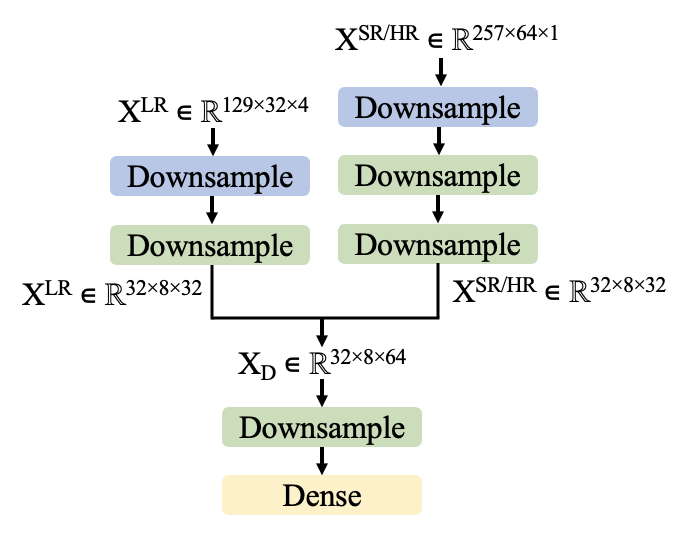
\includegraphics[scale=.24]{thesis/figures/discriminator_left.png}}
        \caption{Conditional discriminator inclusive low-resolution range-Doppler map as condition}
        \label{discriminator inclusive low resolution image as input}
    \end{subfigure}
    \begin{subfigure}{0.49\textwidth}
        \centering
        \adjustbox{height=7cm}{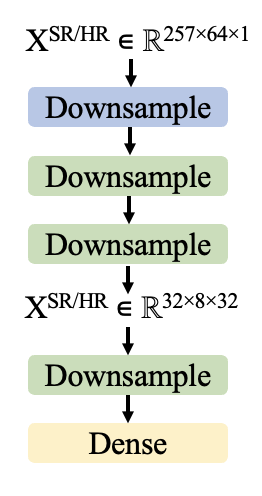
\includegraphics[scale=.24]{thesis/figures/discriminator_right.png}}
        \caption{Discriminator exclusive low-resolution range-Doppler map as input}
        \label{discriminator exclusive low resolution image as input}
    \end{subfigure}
    \caption{The structures of the discriminator in terms of the input}
	\label{structures of the discriminator}
\end{figure}

\begin{figure}
	\centering
	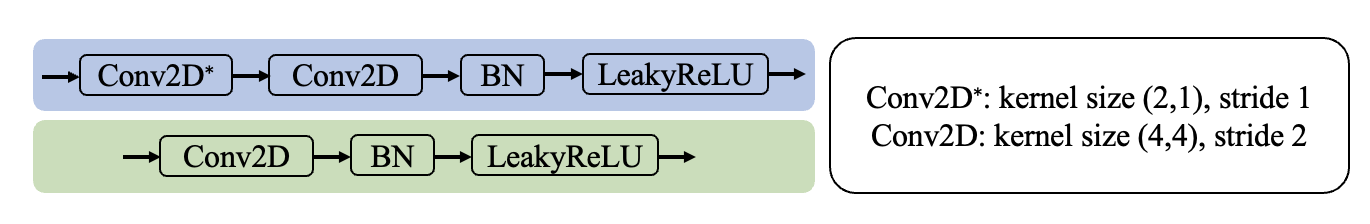
\includegraphics[scale=.62]{thesis/figures/discriminator_downsample.png}
	\caption{Downsample block in the discriminator}
	\label{downsample block in discriminator}
\end{figure}

\chapter{Loss functions} \label{loss functions}
In order to train the model with different settings, we tried many loss functions. This chapter will show all the loss functions used. The loss functions will be slightly different depending on the process, namely for the training and evaluation phases. There are a total of eight loss functions and their combined loss functions.

\section{MSE loss} \label{mse loss}
% show the MSE \& weighted MSE
\gls{mse} is a common loss function in machine learning. Its formula is written as
\begin{equation}
    \centering
    \mathcal{L}_{\text{MSE}} = \frac{1}{n} \sum_{i=1}^{n} (Y_i - \hat{Y}_i)^2,
\end{equation}

where $Y_i$ represents the ground truth, $\hat{Y}_i$ denotes the prediction and $n$ is the total number of the samples. $\mathcal{L}_{\text{MSE}}$ represents the \gls{mse} loss between the ground truth and prediction, and the goal of the model is to reduce this value. 

But in specific cases, the meaning of $Y_i$ and $\hat{Y}_i$ and the usage of this loss function will be different, that is, the format of the values in ground truth and prediction is depending on the processing methods, namely the red part shown in Figure \ref{postprocessing_block}. Furthermore, it can be formulated into two loss functions according to the needs in the range-Doppler map upsampling task, namely \gls{mse} and \gls{wmse}.

\subsection{MSE} \label{mse subsection}
In normal \gls{mse}, no additional weights are added to the loss function, but it is still performed depending on the different processes, training or evaluation phase.

\begin{spacing}{1.5}
\textbf{\large{Training\&validation phases}}
\end{spacing}
In the phase of training and validation, the meaning of the $Y_i$ and $\hat{Y}_i$ is firstly up to the input data representation, that is, in the case of real and imaginary representation type, the loss of both real and imaginary parts will be calculated separately, where $Y_i$ refers to them of the high-resolution data and $\hat{Y}_i$ denotes that of the super-resolution data accordingly, then both will be combined in the way of
\begin{equation}
    \centering
    \mathcal{L}_{\text{MSE}} = \mathcal{L}_{\text{MSE, Re}} + \mathcal{L}_{\text{MSE, Im}},
\end{equation}

whereas in the case of amplitude and phase representation type, the loss of amplitude and phase will be calculated respectively and combined as
\begin{equation}
    \centering
    \mathcal{L}_{\text{MSE}} = \mathcal{L}_{\text{MSE, Amp}} + \lambda \times \mathcal{L}_{\text{MSE, Ph}},
\end{equation}

where $\lambda$ as a hyperparameter can be tuned according to the processing methods. But if only amplitude, then the phase \gls{mse} loss will be neglected.

\begin{spacing}{1.5}
\textbf{\large{Evaluation phases}}
\end{spacing}
Since a lot of settings and combinations exist, in order to make the evaluation fair for all the cases and due to the importance of the amplitude in the range-Doppler map upsampling, only the amplitude loss will be taken into consideration, that is,
\begin{equation}
    \centering
    \mathcal{L}_{\text{MSE, Amp}} = \frac{1}{n} \sum_{i=1}^{n} (A_i - \hat{A}_i)^2,
\end{equation}

where $A$ and $\hat{A}$ are the amplitude of the high-resolution and super-resolution data, respectively. Note that in the training phase, the training loss is calculated between ground truth $Y$ and prediction $\hat{Y}$ which are before the postprocessing block as shown in Figure \ref{postprocessing_block}. However, in the evaluation phase, the amplitude of the ground truth $A$ and prediction $\hat{A}$ are converted back after the postprocessing block.

\subsection{WMSE}
The large dynamic range of radar signal amplitudes  causes relatively low MSE loss for weak signal parts in comparison to strong reflections. The model will not pay much attention on these signals. Therefore, we assign different weights according to the amplitude of the signal. In order to make the weaker signal also get enough attention and the weaker signals get a larger weight, and the formula of amplitude \gls{wmse} loss will become
\begin{equation}
    \centering
    \mathcal{L}_{\text{WMSE, Amp}} = \frac{1}{n} \sum_{i=1}^{n} \frac{(A_i - \hat{A}_i)^2}{A_i},
    \label{amplitude wmse loss equation}
\end{equation}

while the angle loss in \gls{wmse} is still same as in the \gls{mse} and combine them with an additional weight $\lambda$ as well in the case of the amplitude and phase representation type, namely
\begin{equation}
    \centering
    \mathcal{L}_{\text{WMSE}} = \mathcal{L}_{\text{WMSE, Amp}} + \lambda \times \mathcal{L}_{\text{MSE, Ph}},
\end{equation}

while in the evaluation process, only the amplitude loss part, namely formula \ref{amplitude wmse loss equation}, is used. The reason is same as the explanation in the section \ref{mse subsection}.

\section{SDR loss} \label{sdr loss}
% show the SDR \& SD-SDR
In the field of signal processing, a very important indicator is \gls{snr}. We hope to get a larger signal related to the noise. According to the paper \cite{roux_sdr_2018} by Jonathan et al., the classical \gls{snr} is equivalent to the \texttt{bss\_eval\_images}’s SDR in the case that there's only noise between the ground truth $A$ and prediction $\hat{A}$, that is, 
\begin{equation}
    \centering
    \mathcal{L}_{\text{SDR}} = 10 \log_{10} \left( \frac{\|A\|^2}{\|A - \hat{A}\|^2} \right).
    \label{sdr equation}
\end{equation}

As shown in Figure \ref{illustration of the snr and si-sdr}, Jonathan et al. proposed two loss functions as the variations of the \gls{sdr}, called \gls{si-sdr} and \gls{sd-sdr}, which are respectively written as
\begin{equation}
    \centering
    \mathcal{L}_{\text{SI-SDR}} = 10 \log_{10} \left( \frac{\| e_{\text{target}} \|^2}{\| e_{\text{res}} \|^2} \right) = 10 \log_{10} \left(\frac{\left\| \frac{\hat{Y}^{T} Y}{\|Y\|^2} Y \right\|^2}{\left\| \frac{\hat{Y}^{T} Y}{\|Y\|^2} Y - \hat{Y} \right\|^2}\right),
\end{equation}

\begin{equation}
    \centering
    \mathcal{L}_{\text{SD-SDR}} = 10 \log_{10} \left( \frac{\|\alpha s\|^2}{\|s - \hat{s}\|^2} \right) = \mathcal{L}_{\text{SDR}} + 10 \log_{10} \alpha^2,
\end{equation}

where the optimal scaling factor is $\alpha = \hat{Y}^{T} Y / \|Y\|^2$. The advantage of these two variations is the faster convergence, but the \gls{si-sdr} is sensitive to the scaling and \gls{sd-sdr} is not sure in the frequency domain. Therefore, we keep using the classical \gls{sdr} loss, namely formula \ref{sdr equation}. Moreover, the current \gls{sdr} is better when it's larger, so to make it decrease during the training process, a negative sign is added.

\begin{figure}
	\centering
	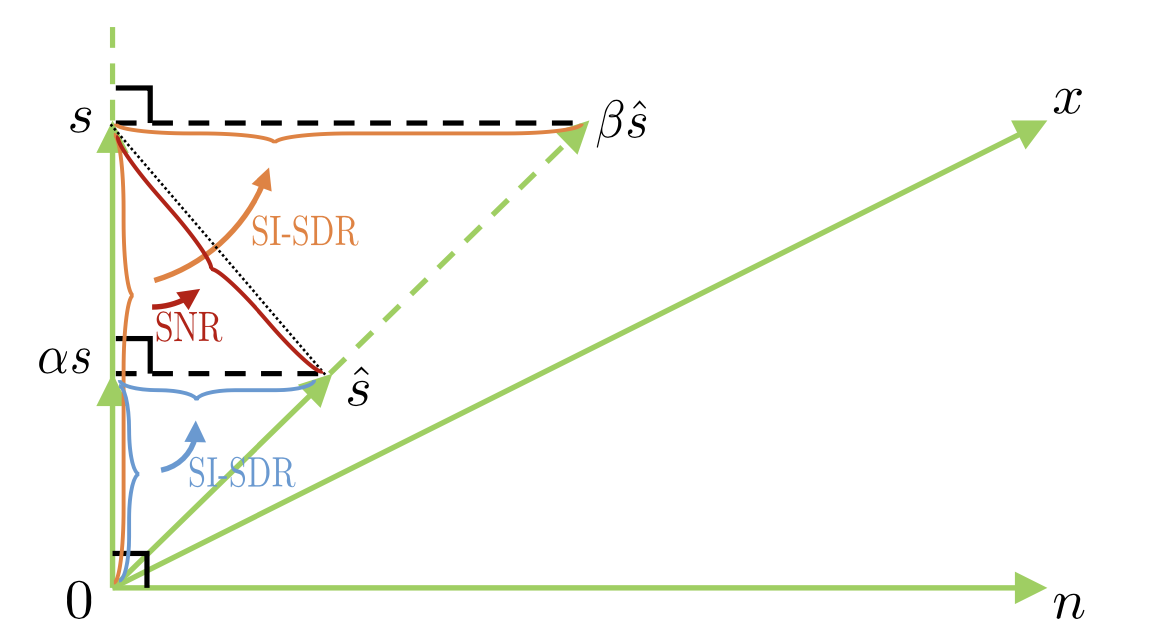
\includegraphics[scale=.55]{thesis/figures/sdr.png}
	\caption{Illustration of the SNR and SI-SDR \cite{roux_sdr_2018}}
	\label{illustration of the snr and si-sdr}
\end{figure}

\section{LSD loss} \label{lsd loss}
% show the LSD and PLSD
Braun et al. proposed two loss functions \cite{braun_consolidated_2020}, \gls{lsd} and \gls{plsd}, which add logarithmic operation on the amplitude compared to classical \gls{mse} and are beneficial for the range-Doppler maps with the significant amplitude fluctuation.

\subsection{LSD}
\gls{lsd} can be described as
\begin{equation}
    \centering
    \mathcal{L}_{\text{LSD, Amp}} = \left\langle \left| \log_{10} \hat{A} - \log_{10} A \right|^2 \right\rangle,
\end{equation}

where $A$ represents the amplitude of each point in the range-Doppler map and
\begin{equation}
    \centering
    \left\langle P(h, w) \right\rangle = \frac{1}{H W} \sum_{h,w} P(h, w).
\end{equation}

To improve the stability further, the root mean square operation can combine with the \gls{lsd} loss function, it turns to
\begin{equation}
    \centering
    \mathcal{L}_{\text{LSD, Amp}} = \left\{ \frac{1}{N} \sum_{n=1}^{N} \left[ \log_{10} A(n) - \log_{10} \hat{A}(n) \right]^p \right\}^{\frac{1}{p}},
    \label{final lsd equation}
\end{equation}

where $p$ is set as 2. With the use of logarithmic operations, the amplitude change will be obviously reduced. However, since the data with high amplitude in the range-Doppler map is relatively only a small part while the part in the longer range or velocity in range-Doppler map occupy the majority, the model will pay much attention on the background noise during the training process, affecting the final super-resolution range-Doppler map. Therefore, a mask is added on the \gls{lsd} loss to ignore much background noise during the training process. The threshold is set according to the median value or the percentile, only the loss of the part which has the amplitude over the threshold will be taken into consideration, otherwise will be neglected. The mask is still based on the logarithm amplitude. If the percentile is set as 50\%, i.e. 50\% data can over the threshold, the mask looks like Figure \ref{mask in the percentile of 70}, where Figure \ref{high resolution image with logarithic amplitude} shows the corresponding high-resolution range-Doppler map with the logarithmic amplitude and Figure \ref{masked high resolution image with logarithic amplitude} illustrates the masked high-resolution range-Doppler map.

\begin{figure}
    \centering
    \hspace{-0.6cm}
    \begin{subfigure}{0.32\textwidth}
        \centering
        \adjustbox{height=3cm}{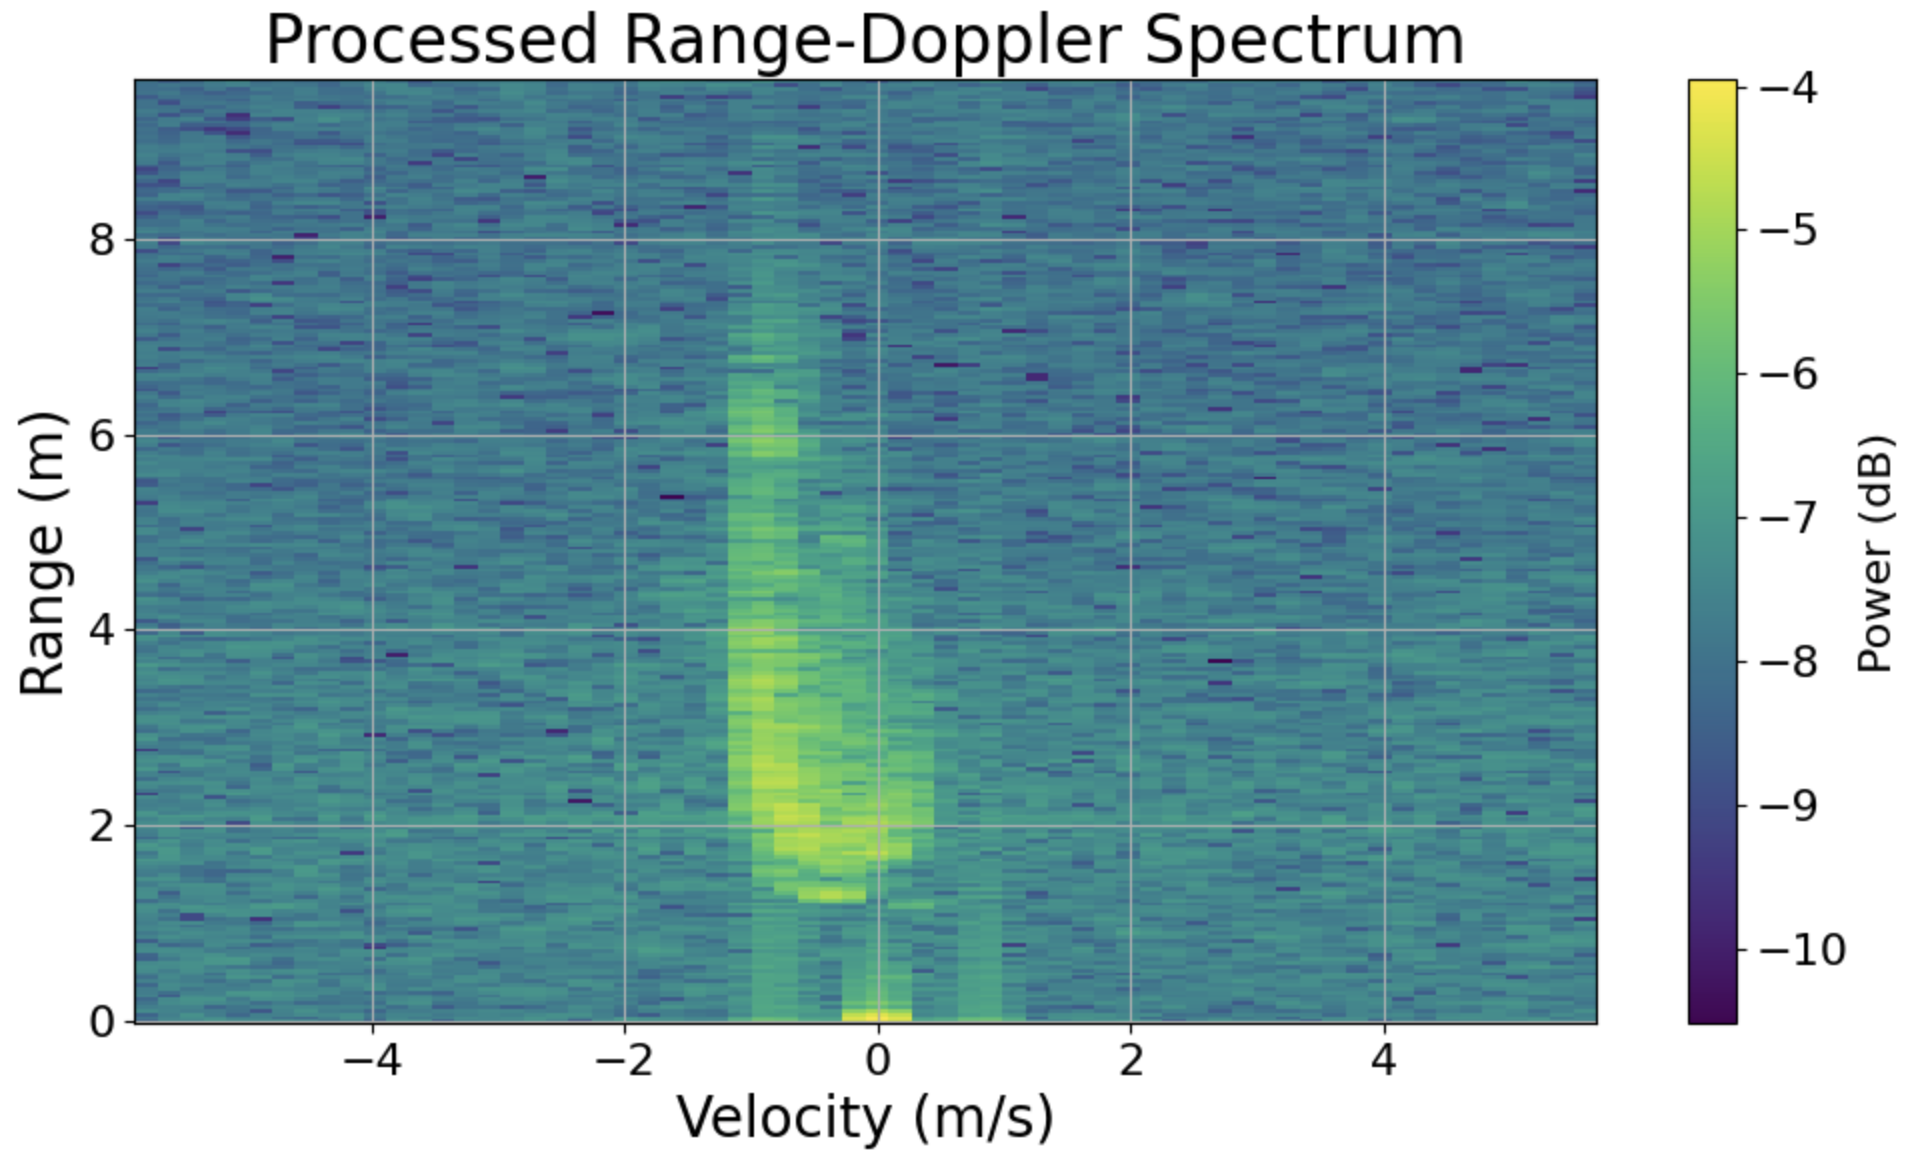
\includegraphics[scale=.24]{thesis/figures/gt_logamp.png}}
        \caption{Processed high-resolution range-Doppler map}
        \label{high resolution image with logarithic amplitude}
    \end{subfigure}
    \begin{subfigure}{0.32\textwidth}
        \centering
        \adjustbox{height=3cm}{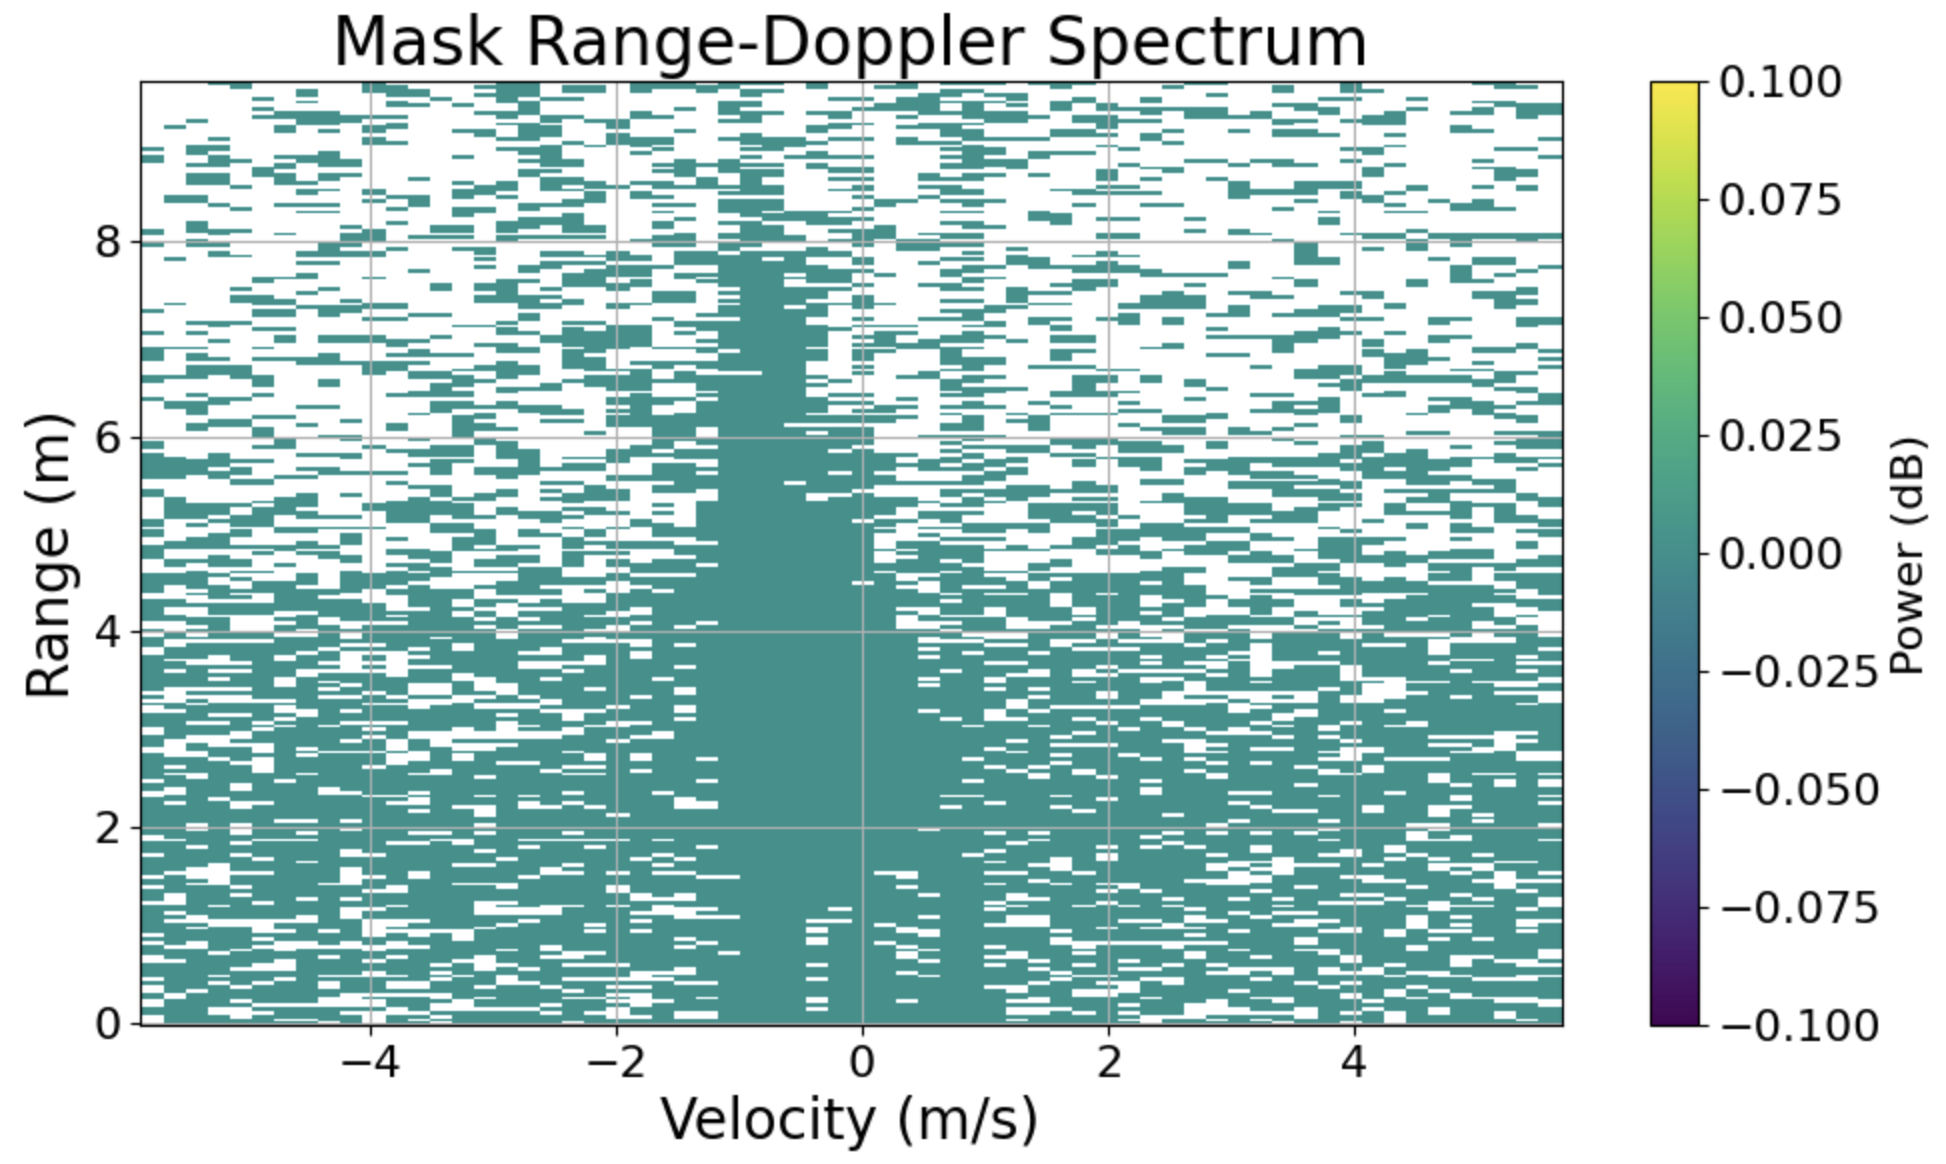
\includegraphics[scale=.24]{thesis/figures/mask.png}}
        \caption{The mask in the percentile of 50\%}
        \label{mask in the percentile of 70}
    \end{subfigure}
    \begin{subfigure}{0.32\textwidth}
        \centering
        \adjustbox{height=3cm}{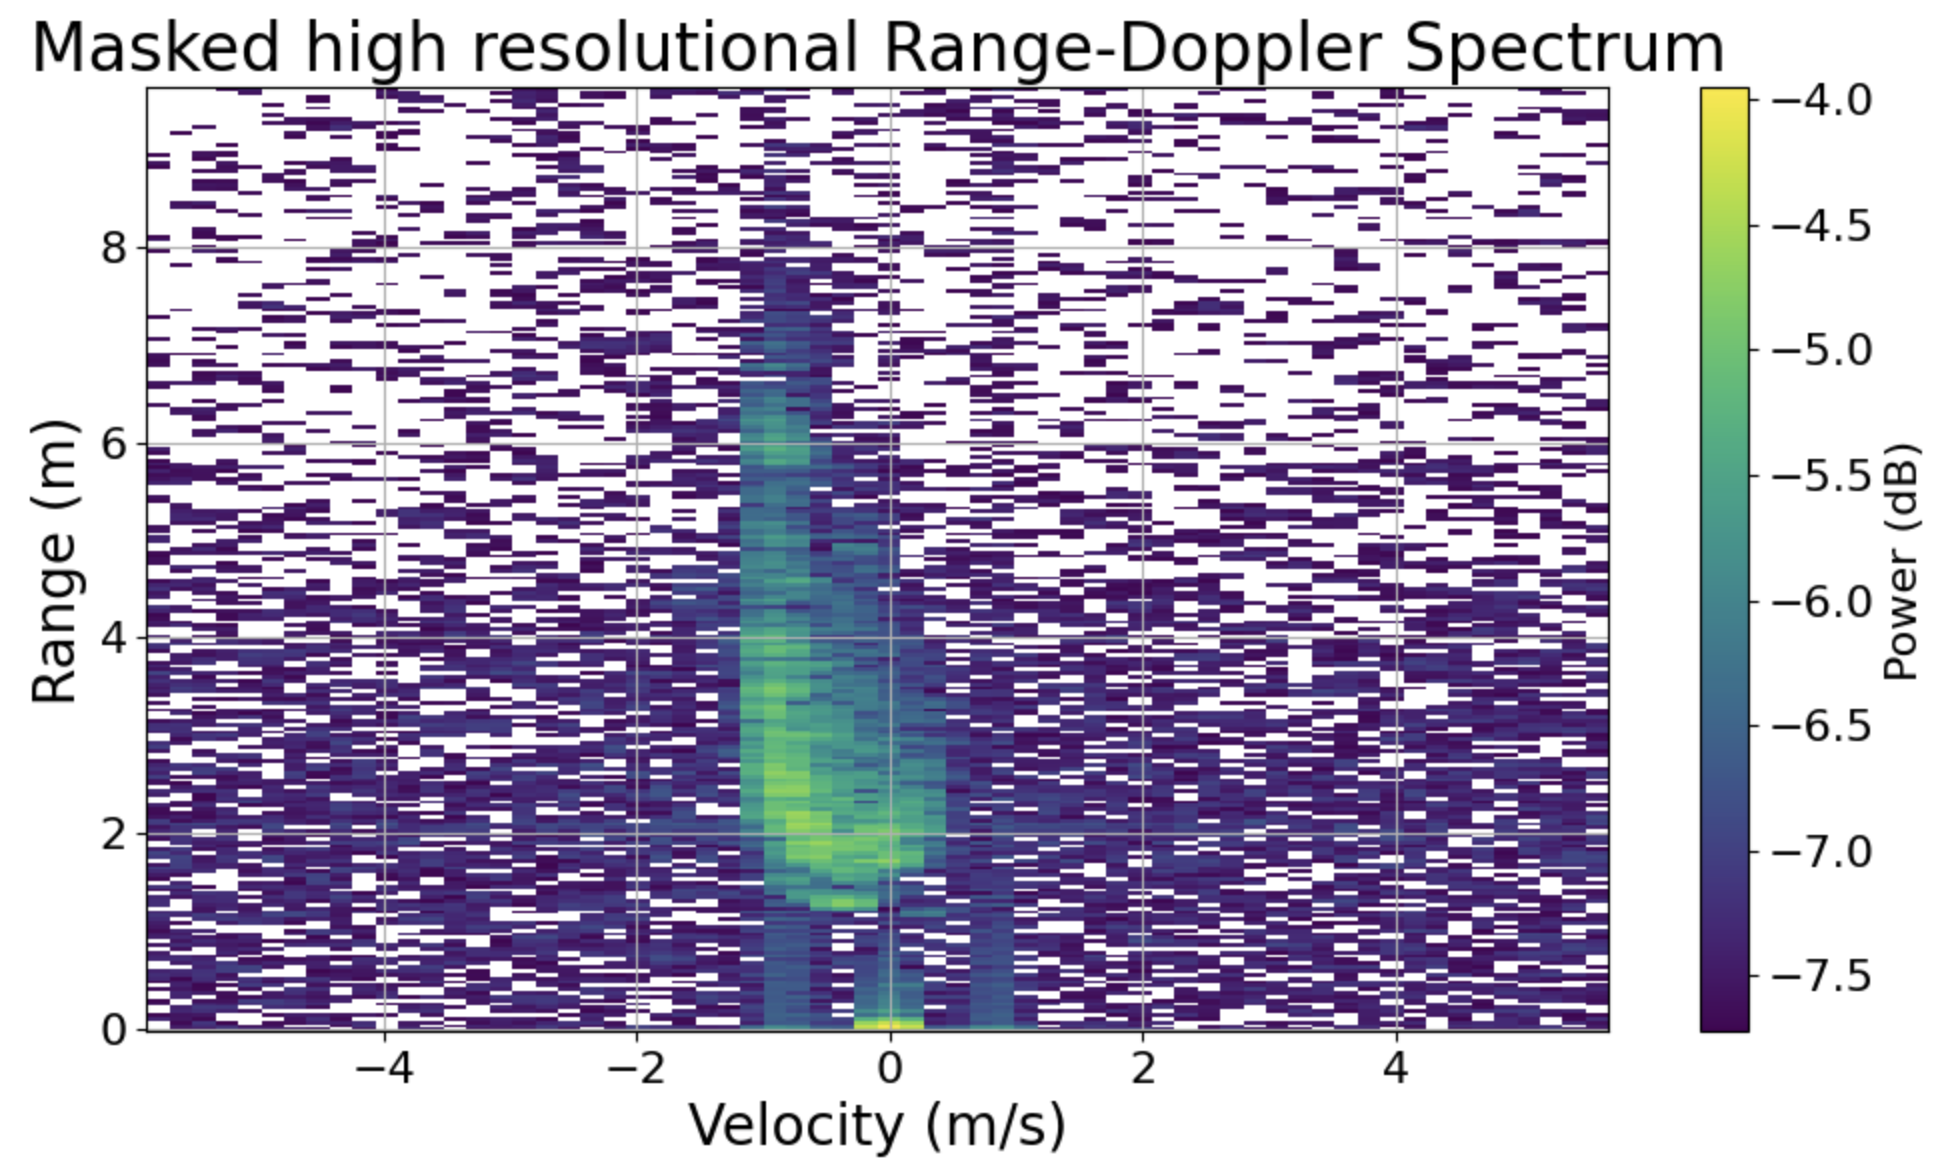
\includegraphics[scale=.24]{thesis/figures/masked_gt.png}}
        \caption{Masked high-resolution range-Doppler map}
        \label{masked high resolution image with logarithic amplitude}
    \end{subfigure}
    \caption{The mask operation on the high-resolution range-Doppler map with logarithic amplitude}
    \label{mask operation on the high resolution image with logarithic amplitude}
\end{figure}

In terms of the phase loss, the \gls{mse} can be used and combined with the scaling factor $\lambda$, namely
\begin{equation}
    \centering
    \mathcal{L}_{\text{LSD}} = \mathcal{L}_{\text{LSD, Amp}} + \lambda \times \mathcal{L}_{\text{MSE, Ph}},
\end{equation}

whereas in the evaluation phase, the scaling factor is set as zero, that is, only the amplitude \gls{lsd} loss is taken into consideration and the mask will not be used. Note that, if in the processing methods the logarithm is performed, both \gls{mse} and \gls{lsd} will have logarithmic operation on the amplitude, then the difference is only the square root in \gls{lsd} loss function. Conversely, if no logarithm operation in the processing methods, the \gls{lsd} loss function keeps using logarithm on the amplitude while the \gls{mse} doesn't have.

\subsection{PLSD}
Compared with the \gls{lsd} loss function, the difference of the \gls{plsd} loss function is that it doesn't use the \gls{mse} phase loss, that is,
\begin{equation}
    \centering
    \mathcal{L}_{\text{PLSD}} = \left\langle \left| \log_{10} \left| \frac{\hat{Y}}{Y} \right| \right| \times \left( 2 - \mathcal{R} \left\{ \frac{\hat{Y}}{Y} \right\} \right) \right\rangle,
\end{equation}

where
\begin{equation}
    \centering
    \mathcal{R} \left\{ \frac{\hat{Y}}{Y} \right\} = \cos{(\varphi_{\hat{Y}} - \varphi_{Y})}.
\end{equation}

\gls{plsd} loss function can be only used in training and validation phases if not amplitude representation type.

\section{Perceptual loss} \label{perceptual loss}
% show the different VGG layer
The \gls{vgg} \cite{simonyan_very_2015} are common models for image reconstruction, which is implemented using multiple blocks of the convolutional layers. Simonyan et al. proposed six \gls{vgg} configurations in different scales, each with the different number of layers and parameters, as shown in Table \ref{vgg configurations}, where the configuration E represents VGG19, which has the most parameters and the highest accuracy.

\begin{table}[t]
    \centering
    \caption{VGG configurations \cite{simonyan_very_2015}}
    \label{vgg configurations}
    % \renewcommand{\arraystretch}{1.3}
    \resizebox{0.99\textwidth}{!}{
    \begin{tabular}{|c|c|c|c|c|c|}
        \hline
        \multicolumn{6}{|c|}{\textbf{VGG Configuration}} \\ 
        \hline
        A & A-LRN & B & C & D & E \\ 
        \hline
        11 weight layers & 11 weight layers & 13 weight layers & 16 weight layers & 16 weight layers & 19 weight layers \\ 
        \hline
        \multicolumn{6}{|c|}{input (224 × 224 RGB image)} \\ 
        \hline
        conv3-64 & conv3-64 & conv3-64 & conv3-64 & conv3-64 & conv3-64 \\ 
          & \textbf{LRN} & \textbf{conv3-64} & conv3-64 & conv3-64 & conv3-64 \\ 
        \hline
        \multicolumn{6}{|c|}{maxpool} \\ 
        \hline
        conv3-128 & conv3-128 & conv3-128 & conv3-128 & conv3-128 & conv3-128 \\ 
          &   & \textbf{conv3-128} & conv3-128 & conv3-128 & conv3-128 \\ 
        \hline
        \multicolumn{6}{|c|}{maxpool} \\ 
        \hline
        conv3-256 & conv3-256 & conv3-256 & conv3-256 & conv3-256 & conv3-256 \\ 
        conv3-256 & conv3-256 & conv3-256 & conv3-256 & conv3-256 & conv3-256 \\ 
          &   &   & \textbf{conv1-256} & \textbf{conv3-256} & conv3-256 \\ 
          &   &   &   &   & \textbf{conv3-256} \\ 
        \hline
        \multicolumn{6}{|c|}{maxpool} \\ 
        \hline
        conv3-512 & conv3-512 & conv3-512 & conv3-512 & conv3-512 & conv3-512 \\ 
        conv3-512 & conv3-512 & conv3-512 & conv3-512 & conv3-512 & conv3-512 \\
          &   &   & \textbf{conv1-512} & \textbf{conv3-512} & conv3-512 \\
          &   &   &   &   & \textbf{conv3-512} \\
        \hline
        \multicolumn{6}{|c|}{maxpool} \\ 
        \hline
        conv3-512 & conv3-512 & conv3-512 & conv3-512 & conv3-512 & conv3-512 \\ 
        conv3-512 & conv3-512 & conv3-512 & conv3-512 & conv3-512 & conv3-512 \\
          &   &   & \textbf{conv1-512} & \textbf{conv3-512} & conv3-512 \\
          &   &   &   &   & \textbf{conv3-512} \\
        \hline
        \multicolumn{6}{|c|}{maxpool} \\ 
        \hline
        \multicolumn{6}{|c|}{FC-4096} \\  
        \hline
        \multicolumn{6}{|c|}{FC-4096} \\ 
        \hline
        \multicolumn{6}{|c|}{FC-1000} \\ 
        \hline
        \multicolumn{6}{|c|}{soft-max} \\ 
        \hline
    \end{tabular}
    }
\end{table}

Johnson et al. proposed a perceptual loss function based on the \gls{vgg} model, using the features extracted from different layers of the VGG model to calculate the loss between super-resolution and high-resolution data \cite{johnson_perceptual_2016}. Compared with the per-pixel loss function mentioned above, perceptual loss function can produce a more visually pleasing range-Doppler map. They proposed two types of the perceptual loss functions, one is about the feature reconstruction loss which is the Euclidean distance between the feature representation
\begin{equation}
    \centering
    \mathcal{L}_{\text{Perceptual}} (\hat{Y}, Y) = \frac{1}{H W C} \left\| \phi (\hat{Y}) - \phi (Y) \right\|_2^2,
\end{equation}

where $\phi(\cdot)$ denotes the feature extraction of the \gls{vgg} model and another type is based on the style of the image, namely
\begin{equation}
    \centering
    G^{\phi}(x)_{c, c'} = \frac{1}{H W C} \sum_{h=1}^{H} \sum_{w=1}^{W} \phi (\hat{Y})_{h,w,c} \phi (Y)_{h,w,c'}.
\end{equation}

In our case, the upsampling data is specifically the range-Doppler map, therefore, the feature reconstruction perceptual loss is used rather than the style. In \gls{vgg} model, with the deeper channel of blocks, the representation of each block changes. In the first two blocks, the shallow features are learned, such as margin, color and brightness. Since the third block, more deeper feature are represented, such as texture. And in fourth and fifth blocks, some distinguished features are extracted. Therefore, in the perceptual loss function of the pipeline, the last layer of the first four blocks in the pretrained \gls{vgg} model provided by TensorFlow are used to extract the feature representation by default, since it can mitigate the loss computation to be much expensive. Furthermore, since the channel dimension of the range-Doppler map is just one, while in the \gls{vgg} model, RGB image is used for pretraining, the range-Doppler map has to extend the channel dimension.

\section{Combination of the losses} \label{combination of the losses}
% combination of the loss functions such as LSD+Perceptual loss functions, as well as the pre-training with the single loss function firstly while combination.
According to the various loss functions mentioned above, their types and goals are somewhat different. For example, \gls{lsd} loss function uses logarithmic operations to pay more attention on the signal with low amplitude, while the perceptual loss function improves the overall perception of the range-Doppler map using the feature representation. Therefore, different types of loss functions can be combined with each other, such as
\begin{equation}
    \centering
    \mathcal{L}_{\text{Combination}} = \mathcal{L}_{\text{LSD}} + \lambda_c \times \mathcal{L}_{\text{Perceptual}},
    \label{loss combination equation}
\end{equation}

where $\lambda_c$ as a hyperparameter that can be tuned according to the importance or the values of both loss functions. Moreover, in order to improve the stability, the pretraining operation can be used, that is, the model can be trained with one loss of the loss combination and after a few epochs trained by both. Otherwise, at the very beginning of the training, if the perceptual loss is relatively large, it would cause too much attention on the perception rather than the target \gls{lsd} loss per pixels.

\section{Adversarial loss} \label{gan loss}
% show both generator loss and discriminator loss
In \gls{cgan} model, the generator and discriminator models will be trained mutually, whereas the loss functions for both are different. Therefore in this section, the generator loss function and discriminator loss function will be shown respectively.

\subsection{Generator loss}
For the generator model, on one hand, it should reduce the value of the loss combination, such as the \gls{lsd} combining with perceptual loss, after multiple epochs of training, and on the other hand, it should make the discriminator believe that the super-resolution range-Doppler map is the real high-resolution range-Doppler map. Since the output of the discriminator model is a probability value, the adversarial loss for the generator part should be regarded as the difference between this probability and 100\%, that is,
\begin{equation}
    \centering
    \mathcal{L}_{\text{GAN, Gen}} = \| 1 - P_{\text{Super}} \|_{2},
\end{equation}

where $P_{\text{Super}}$ represents the probability value of the super-resolution range-Doppler map as the real high-resolution range-Doppler map from the discriminator model. The total generator loss function should combine with the target loss function mentioned above, namely
\begin{equation}
    \centering
    \mathcal{L}_{\text{Gen}} = \mathcal{L}_{\text{Combination}} + \lambda_g \times \mathcal{L}_{\text{GAN, Gen}},
\end{equation}

\subsection{Discriminator loss}
For the discriminator model, its goal is to make the probability of identifying the super-resolution and ground truth as real high-resolution range-Doppler maps approaching 0 and 1 respectively. Therefore, the discriminator loss function also contains two parts, namely
\begin{equation}
    \centering
    \mathcal{L}_{\text{Disc}} = \| 1 - P_{\text{High}} \|_{2} + \| 0 - P_{\text{Super}} \|_{2},
\end{equation}

where $P_{\text{High}}$ is the probability value that the ground truth is really the high-resolution range-Doppler map.


\chapter{Training optimization} \label{training optimization}
In this chapter, the methods and settings to optimize the training process in the pipeline are shown, including but not limited to distributed training, early stopping, learning rate schedule and hyperparameter tuning.

\section{Distributed training} \label{distributed training}
In order to make full use of multiple \gls{gpu}s for training and speed up the training process, TensorFlow provides the distributed training \gls{api} to achieve parallel computing across multiple GPUs, machines or TPUs. Depending on the device, the strategy has five types, as shown in Table \ref{overview of the distributed training strategies in tensorflow}.

\begin{table}
    \centering
    \caption{Overview of the distributed training strategies in TensorFlow \cite{noauthor_distributed_nodate}}
    \label{overview of the distributed training strategies in tensorflow}
    \begin{tabular}{l|c|c|c|c|c}
        \hline
        \textbf{\makecell[l]{Training\\ API}} & \textbf{\makecell[c]{Mirrored \\ Strategy}} & \textbf{TPUStrategy} & \textbf{\makecell[c]{MultiWorker-\\ Mirrored\\ Strategy}} & \textbf{\makecell[c]{CentralStorage\\ Strategy}} & \textbf{\makecell[c]{ParameterServer\\ Strategy}} \\
        \hline
        \makecell[l]{Keras\\ Model.fit} & Supported & Supported & Supported & \makecell[c]{Experimental\\ Supported} & \makecell[c]{Experimental\\ Supported} \\
        \hline
        \makecell[l]{Custom\\ training\\ loop} & Supported & Supported & Supported & \makecell[c]{Experimental\\ Supported} & \makecell[c]{Experimental\\ Supported} \\
        \hline
        \makecell[l]{Estimator\\ API} & \makecell[c]{Limited\\ Support} & \makecell[c]{Not\\ Supported} & \makecell[c]{Limited\\ Support} & \makecell[c]{Limited\\ Support} & \makecell[c]{Limited\\ Support} \\
        \hline
    \end{tabular}
\end{table}

According to the case in our pipeline, the custom training loop is chosen and multiple GPUs with the same model in the same machine for each training are used, so the mirrored strategy is more in line with our needs. The principle is illustrated in Figure \ref{illustration of the mirrored distributed training strategy}, that is, it will divide the mini-batch data equally by the number of \glspl{gpu} into each \gls{gpu}, where each small divided data of the mini-batch is called a replica. The \gls{gpu}s contain the same model, and each \gls{gpu} uses the replica for training to update parameters, obtain loss and super-resolution range-Doppler maps. Once all GPUs have completed the training process, the obtained parameters and losses are averaged, and all super-resolution range-Doppler maps can be concatenated, then the training process of a batch of data is finished.

\begin{figure}
	\centering
	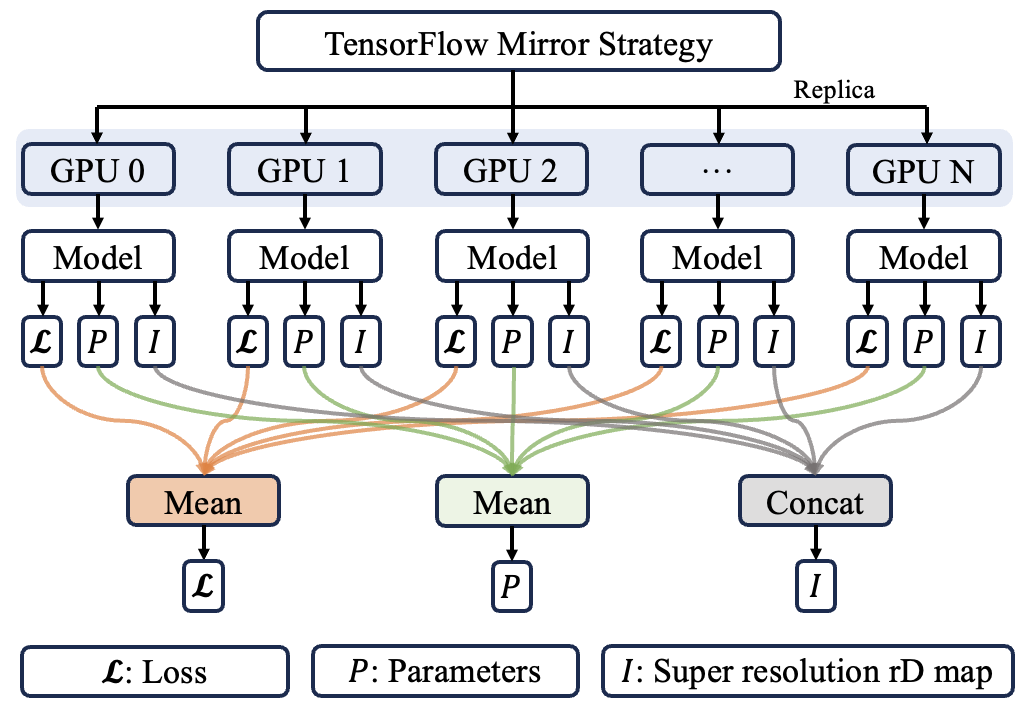
\includegraphics[scale=.65]{thesis/figures/distributed_training.png}
	\caption{Illustration of the mirrored distributed training strategy}
	\label{illustration of the mirrored distributed training strategy}
\end{figure}

Compared with the original custom training loop, the updates in the pipeline are using strategy to load the model and the optimizer, as well as set up the checkpoint. Additionally, the custom training loop should be run as a new loop within the strategy loop, so that the strategy will automatically divide the batch and average the loss and parameters. It is noted that the operation on the loss should be selected as sum by default, since the strategy will then automatically calculate the average of the sum value.

\section{Settings in the pipeline} \label{settings in the pipeline}
In this section, some settings are introduced in order to speed up the training process as well as save the checkpoints for restoring the model in the evaluation phase.

\begin{spacing}{1.5}
\textbf{\large{Early stopping}}
\end{spacing}
In the training loop, the training and validation losses are obtained after each epoch if not pretraining. Otherwise, after pretraining phase, each epoch has a validation loss. By default, the training loop is terminated if the validation loss does not decrease after 10 consecutive epochs to avoid that the training process doesn't have progress due to overfitting but occupies the resources for a long time after setting a higher number of epochs.

\begin{spacing}{1.5}
\textbf{\large{Learning rate schedule}}
\end{spacing}
In order to speed up the training process and adjust the learning rate at different training stages to help the model converge better, the learning rate schedule is used in the pipeline. According to the size of low-resolution training set as \texttt{(28353, 4, 32, 256)}. By default, after every 10,000 batches, the learning rate lowers by factor 0.96 and the initial learning rate as a hyperparameter can be determined according to the different cases. The learning rate goes as shown in Figure \ref{overview of the learning rate schedule} in the case that the number of the epochs is 200.

\begin{figure}
	\centering
	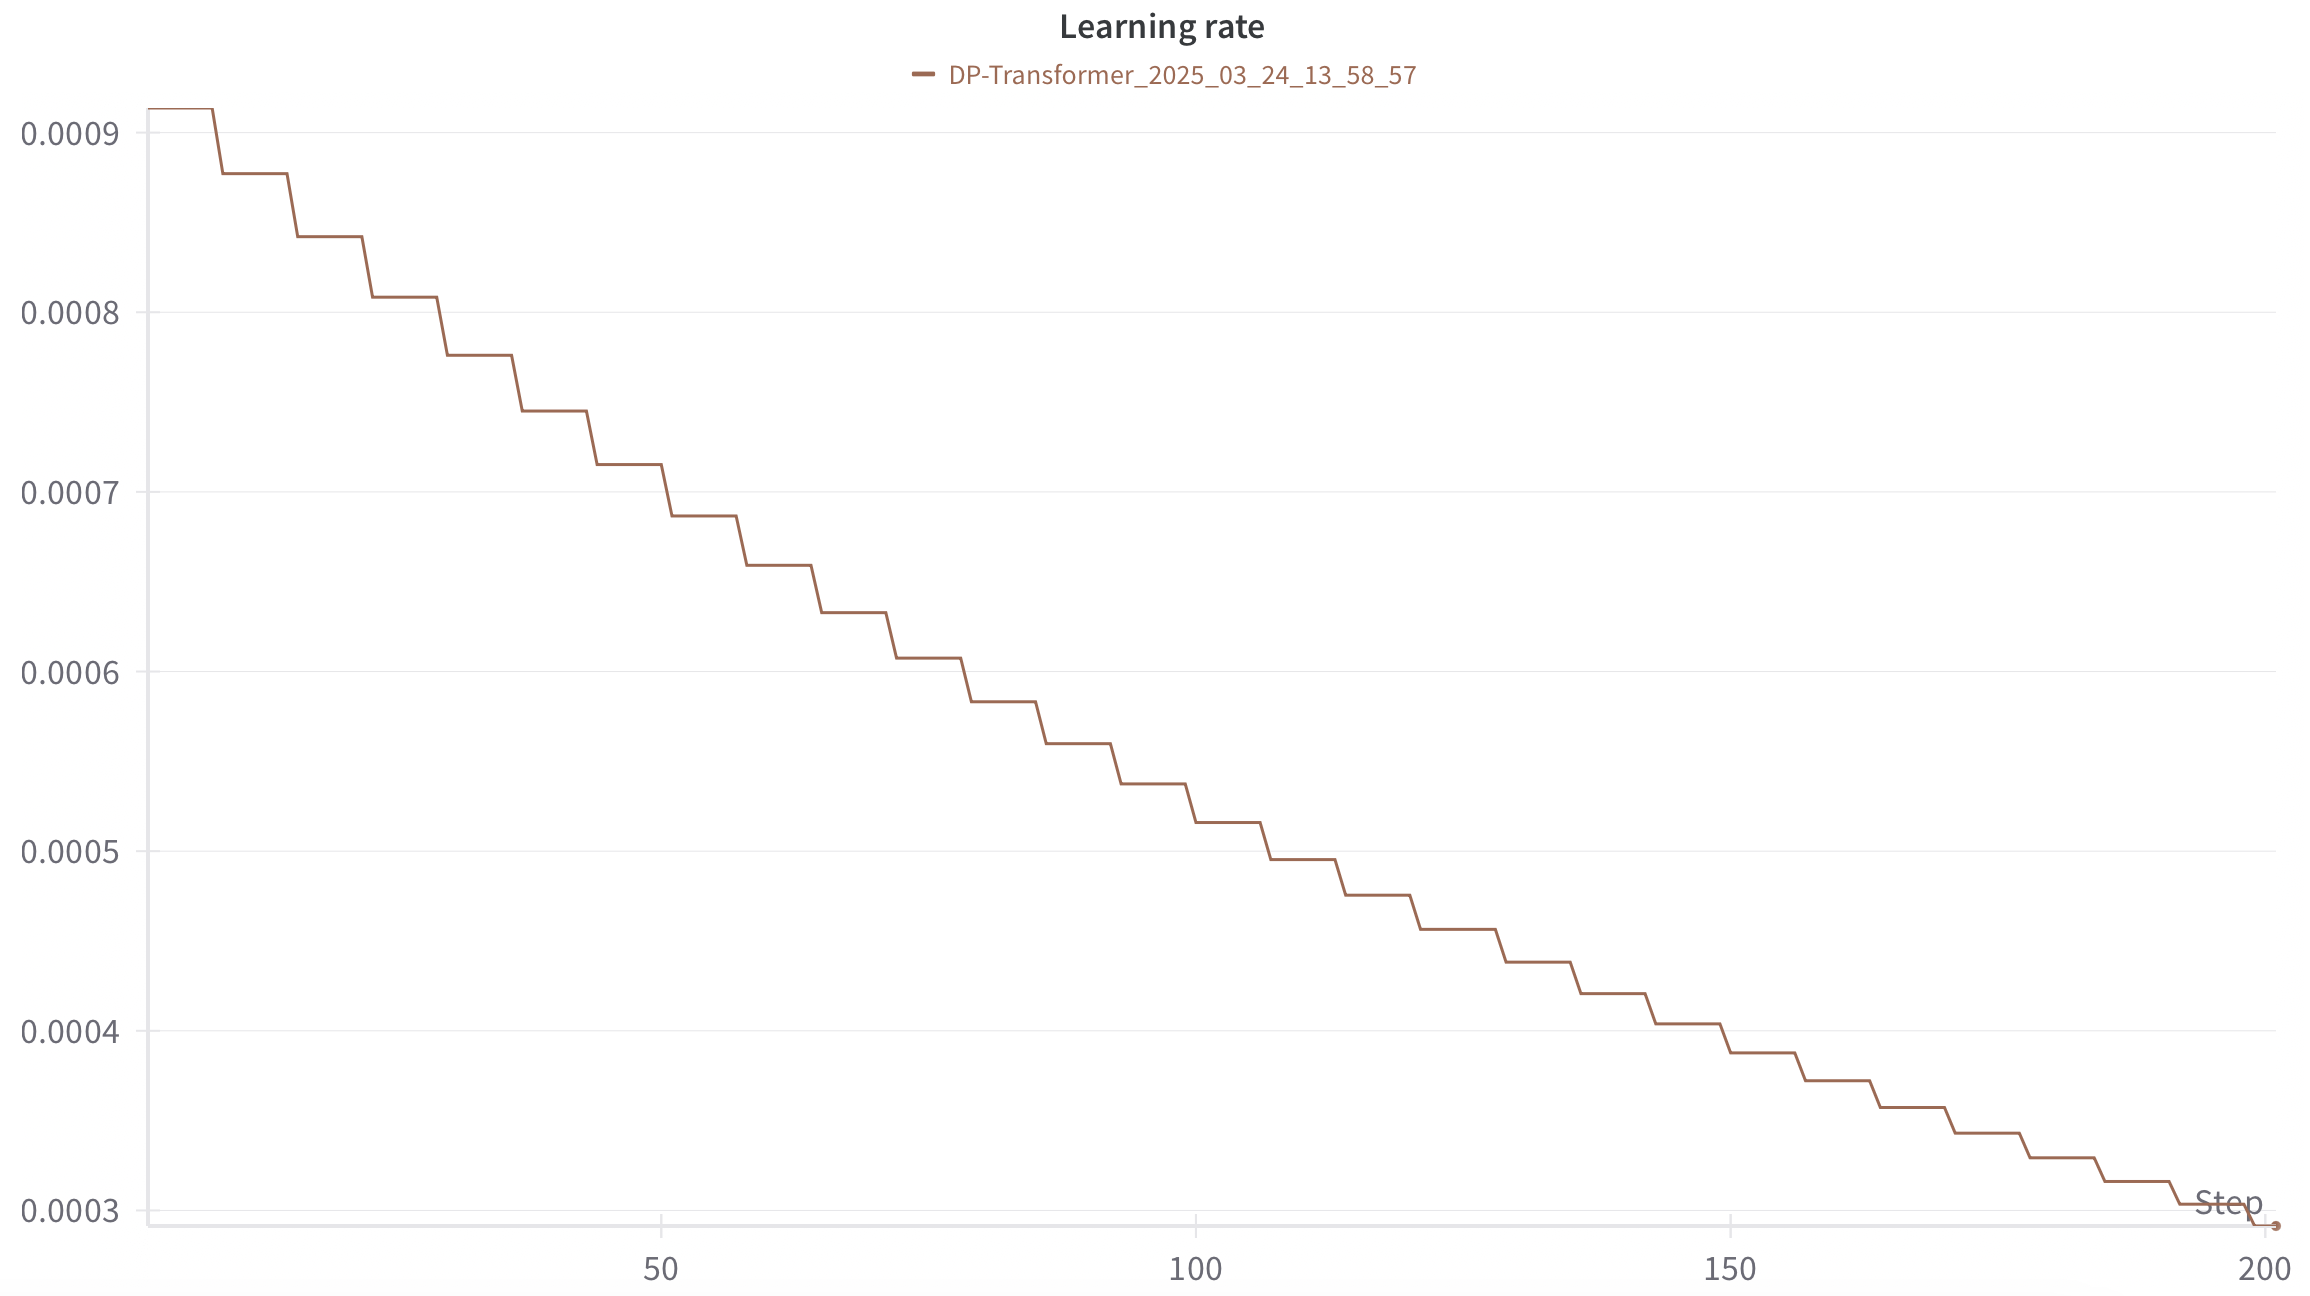
\includegraphics[scale=.3]{thesis/figures/learning_rate_schedule.png}
	\caption{Overview of the learning rate schedule in the case of 200 epochs, decay steps as 10,000, decay rate as 0.96 and initial learning rate as 9.1e-4.}
	\label{overview of the learning rate schedule}
\end{figure}

\begin{spacing}{1.5}
\textbf{\large{Checkpoint setting}}
\end{spacing}
In order to separate the training and evaluation phases and effectively prevent the interruption during the training process, the trainable parameters of the model can be saved in checkpoints. The strategy in the pipeline is by default to save the checkpoint immediately after the first epoch, and then save the current model parameters in the checkpoint as the validation loss decreases in the next epochs. To prevent storing too many checkpoints of the ealier stage, the default setting only retains the latest 5 checkpoints.

\begin{spacing}{1.5}
\textbf{\large{WandB}}
\end{spacing}
\gls{wandb} \cite{wandb_site_2025} is a tool that can be used to track, visualize, and collaborate on machine learning projects. It provides many functions, such as tracking indicators, storing data, tuning hyperparameters, and visualizing models. In our pipeline, \gls{wandb} is mainly used for recording and tuning. In the training loop, \gls{wandb} will record the low-resolution, super-resolution, and high-resolution range-Doppler map of both the training set and validation set in the last batch of each epoch, for a total of six range-Doppler maps. Meanwhile, it records the training loss, validation loss, current best validation loss, learning rate, and running time of each epoch, where Figure \ref{overview of the learning rate schedule} is recorded by \gls{wandb}. Furthermore, \gls{wandb} will automatically record some system usage, such as memory usage, power usage, etc. Additionally, in our pipeline, \gls{wandb} is also used for sweeping the hyperparameters to tune.

\begin{spacing}{1.5}
\textbf{\large{Optimizer}}
\end{spacing}
There are many choices for optimizers, among which \gls{bgd} and \gls{sgd} are the basic optimizers. Then the new methods were designed such as Momentum, which are used to speed up optimization and convergence. After that, optimizers such as \gls{adagrad} and \gls{rmsprop} were proposed, which will optimize the parameters according to the importance, namely larger updates to parameters with low importance but smaller updates to parameters with high importance, which greatly improves robustness as well. The most commonly used optimizer at present is \gls{adam}, which effectively combines the advantages of \gls{rmsprop} and Momentum and achieves better results \cite{kingma_adam_2017}.

In our pipeline, the Adam optimizer is used by default. During the tuning process, the other above-mentioned adaptive optimizers could be tested, such as \gls{rmsprop} and so on. Moreover, there are two \gls{api}s to load optimizer in TensorFlow, where the \texttt{tf.keras.optimizers.legacy} requires a higher version of TensorFlow but can provide faster speed, while the normal \texttt{tf.keras.optimizers} is suitable for lower versions, so the lower version is used by default in the server but can use the faster one in the local computer.

\begin{spacing}{1.5}
\textbf{\large{Pre-training}}
\end{spacing}
Since the training with \gls{vgg} perceptual loss and \gls{cgan} is not stable in the early epochs and in order to make sure that the optimization of the model goes to the ideal direction, we introduced the pretraining phase. As a training loss function is combined with perceptual loss, or when cGAN is used, the training processing will be only affected by the \gls{lsd} loss function in the first 50 epochs by default to ensure the stability in the early stage.


\section{Hyperparameter optimization} \label{hyperparameter optimization}
\gls{wandb} provides a sweep function that can be used to combine different hyperparameters and find the optimal solution based on the goal. In our pipeline, \gls{wandb} will record the best validation loss during training, and hence, the goal is set to minimize this value during tuning. Sweep function provides a variety of combination methods, such as grid, random, and Bayes, among which random combination of the hyperparameters is the most common method. In the pipeline, multiple specified configuration files of each model can be created to save the hyperparameters which are going to be tuned, so that the settings can be modified easily during the tuning process. For the training loop, some settings or hyperparameters can be tuned, such as the type of optimizer, learning rate, batch size, etc. In terms of the models, such as \gls{dp}-\gls{tf} Transformer model, the hyperparameters to be tuned could be the number of filters, the kernel size of encoder and decoder, as well as the number of the blocks, etc.

\chapter{Results} \label{results}
As mentioned in the previous chapters, compared with the upsampling approaches in other papers, this thesis has many updates in the model, data processing and loss function, so this chapter will mainly focus on the evaluation of these three aspects, but also some others. Since only its amplitude is useful in the visualization of range-Doppler map, the evaluation loss will be only based on the amplitude and only in the frequency domain as mentioned in chapter \ref{loss functions}. Furthermore, during the training process, the input of the model may be processed in many different ways, and the pipeline uses the processed output to calculate the training loss, whereas in the evaluation phase, the data will be converted back to the complex value without logarithm and normalization to calculate the evaluation loss.

Since there are too many combinations, in order to make an intuitive and clear comparison, each evaluation will ensure that other parameters are the same, and only one difference will be compared each time, and the most suitable one will be determined for the subsequent evaluations. Due to the large number of evaluation cases, the size of the model and data are selected as a small one, whereas a large model will be trained with the whole dataset at the end. The evaluation indicators are mainly divided into two parts, one is the values of the evaluation losses. The smaller the evaluation loss, the better the model. The other is the visual effect of the generated super-resolution range-Doppler map.

\section{Models comparison} \label{models comparisons}

Firstly, a model shall be determined to evaluate various subsequent processing methods and loss functions. Here, the classical loss function and common processing methods are used, namely the \gls{mse} loss function for training, convolutional layer as the dimension processing layer for the prime range shape and transposed convolutional layer as the upsampling layer, using the real and imaginary representation type, and without any logarithm or normalization operations, that is, the \gls{mse} loss function is calculated in linear scale.

\begin{table}
    \centering
    \caption{Evaluation losses of different models in the case of the MSE and common processing methods.}
    \label{models comparison in the case of the MSE and original processing methods}
    \begin{tabular}{l|c|c|c|c|c|c}
        \hline
        Models comparison & \#Params & MSE & SDR & LSD & WMSE & Perceptual \\
        \hline
        Interpolation & 0 & 3.570 & -3.620 & 0.750 & 0.774 & 28.010 \\
        \hline
        CNN\_simple & 103,684 & 2.164 & -5.028 & \textbf{0.441} & 3.599 & 25.133 \\
        \hline
        UNet\_simple & 93,162 & 1.352 & -2.872 & 0.600 & 1.034 & 22.014 \\
        \hline
        UNet\_concat & 96,746 & \textbf{1.275} & -3.609 & 0.552 & 0.968 & \textbf{21.847} \\
        \hline
        DP & 113,964 & 3.212 & -4.926 & 0.611 & \textbf{0.163} & 23.583 \\
        \hline
        SwinIR+DP & 97,252 & 1.754 & \textbf{-5.787} & 0.503 & 0.314 & 22.764 \\
        \hline
        SwinIR+Swin & 111,624 & 1.541 & -4.505 & 0.546 & 1.104 & 26.381 \\
        \hline
    \end{tabular}
\end{table}

\begin{figure}
    \centering
    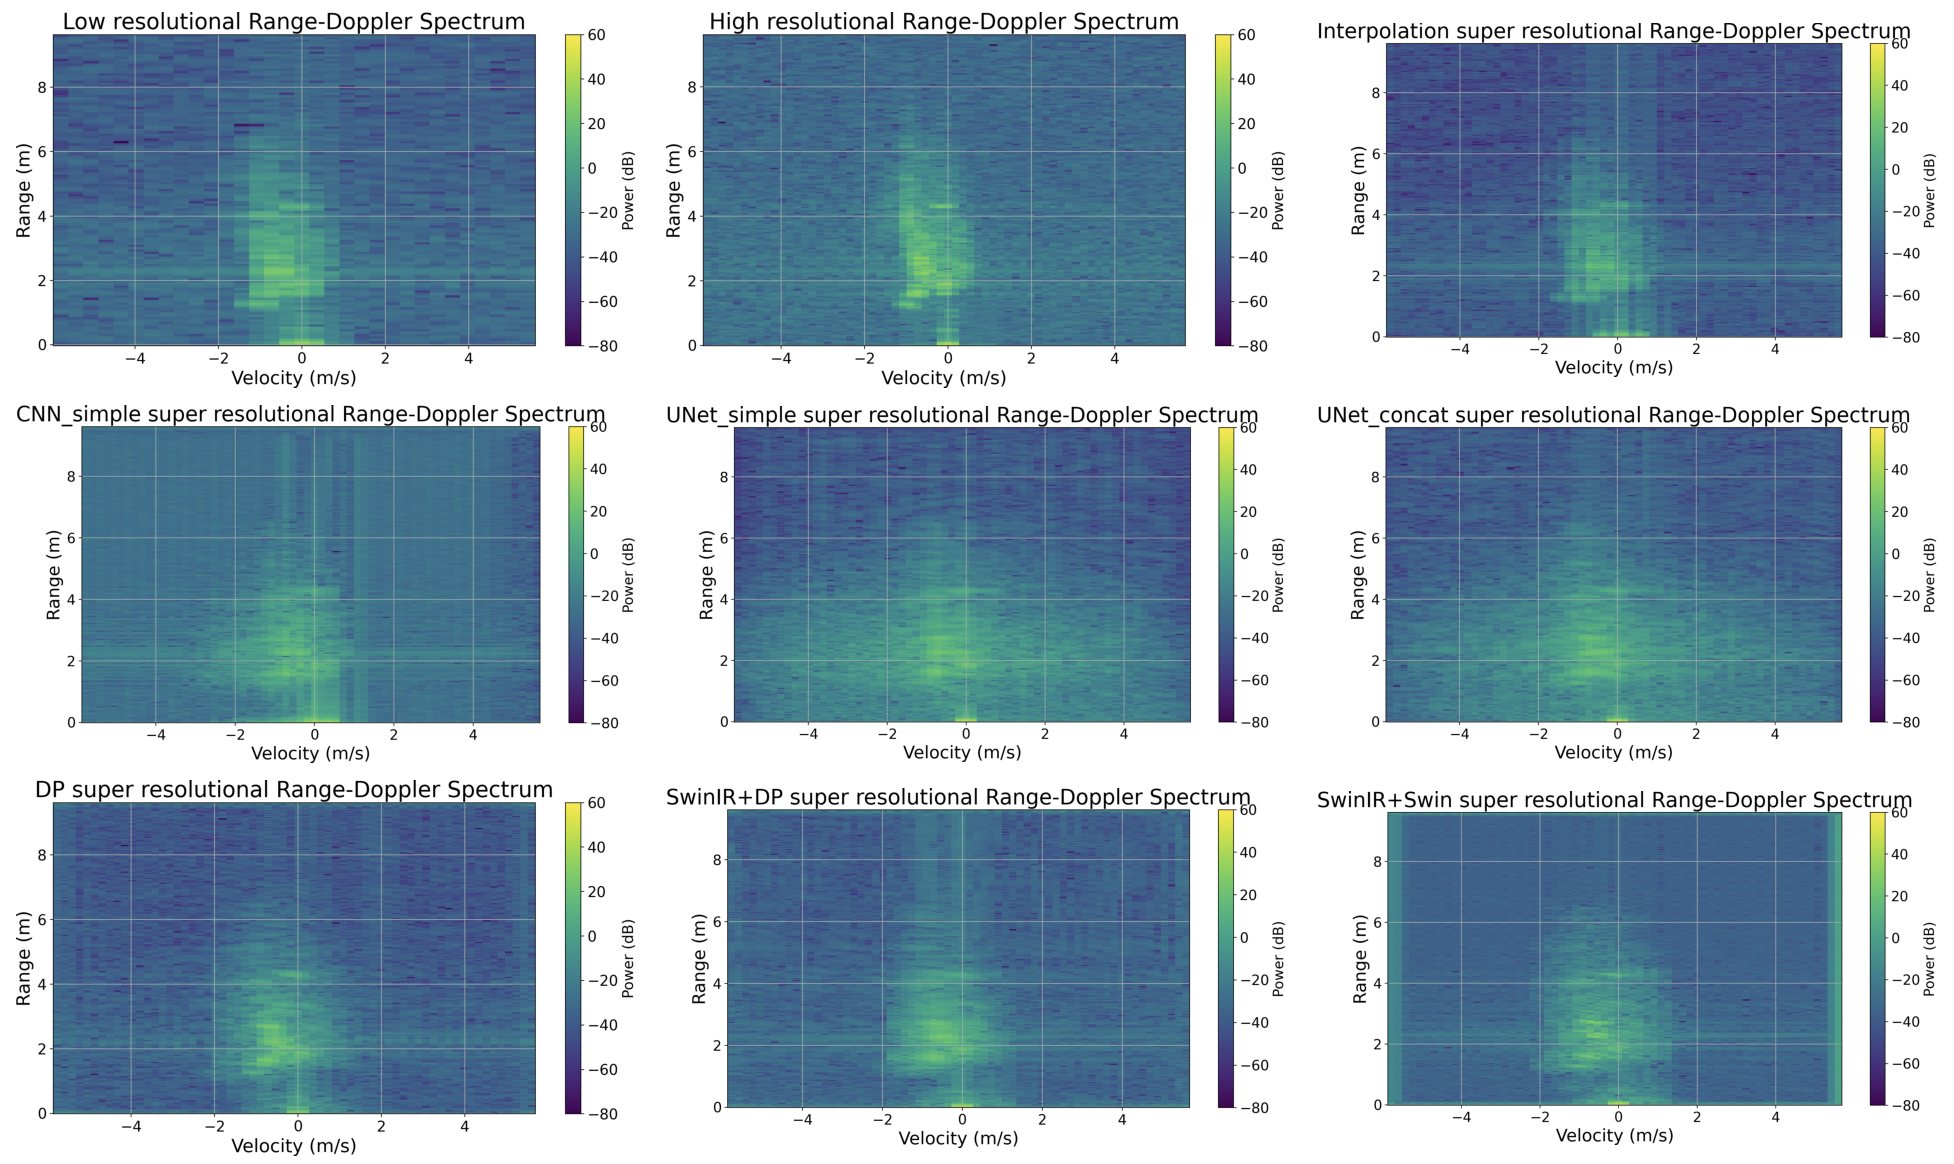
\includegraphics[scale=.45]{thesis/figures/evaluation_models_1.png}
    \caption{Super-resolution range-Doppler maps of different models in the case of the MSE and common processing methods.}
    \label{evaluation models 1}
\end{figure}

From the results of the evaluation losses in Table \ref{models comparison in the case of the MSE and original processing methods}, most models have one good result, but from the perspective of super-resolution range-Doppler maps shown in Figure \ref{evaluation models 1}, the basic \gls{cnn} model and both UNet models are not as good as the Transformer models, since there seems to be some information loss in the area of the strong signals. Among them, the \gls{dp}-\gls{tf} Transformer model and \gls{swinir} architecture with \gls{dp} Transformer block model seem to be better at present. The subsequent evaluations on the processing methods and training loss functions will temporarily use the \gls{dp}-\gls{tf} Transformer model.

According to the optimal processing methods evaluated in section \ref{processing methods comparisons} and the loss combination evaluated in section \ref{training loss functions evaluations}, we evaluate again the models. Table \ref{models comparison in the case of the LSD and new processing methods} and Figure \ref{evaluation models 2} show the evaluation losses and super-resolution range-Doppler maps in the new case.

\begin{table}
    \centering
    \caption{Evaluation losses of different models in the case of the loss combination and new processing methods.}
    \label{models comparison in the case of the LSD and new processing methods}
    \begin{tabular}{l|c|c|c|c|c}
        \hline
        Models comparison & MSE & SDR & LSD & WMSE & Perceptual \\
        \hline
        Interpolation & 2.485 & -6.825 & 0.435 & 1.305 & 21.898 \\
        \hline
        CNN\_simple & 3.574 & -7.722 & 0.345 & 0.227 & 26.649 \\
        \hline
        UNet\_simple & 3.126 & -7.918 & 0.338 & 0.225 & 19.148 \\
        \hline
        UNet\_concat & 1.992 & \textbf{-8.355} & \textbf{0.320} & 0.175 & 17.916 \\
        \hline
        DP & 1.731 & -5.375 & 0.380 & 0.179 & \textbf{12.320 }\\
        \hline
        % DP & 2.052 & -5.530 & 0.377 & 0.192 & 11.997 \\
        % \hline
        SwinIR+DP & 1.662 & -6.415 & 0.360 & \textbf{0.128} & 16.903 \\
        \hline
        SwinIR+Swin & \textbf{1.619} & -6.392 & 0.360 & 0.134 & 15.662 \\
        \hline
    \end{tabular}
\end{table}

\begin{figure}
    \centering
    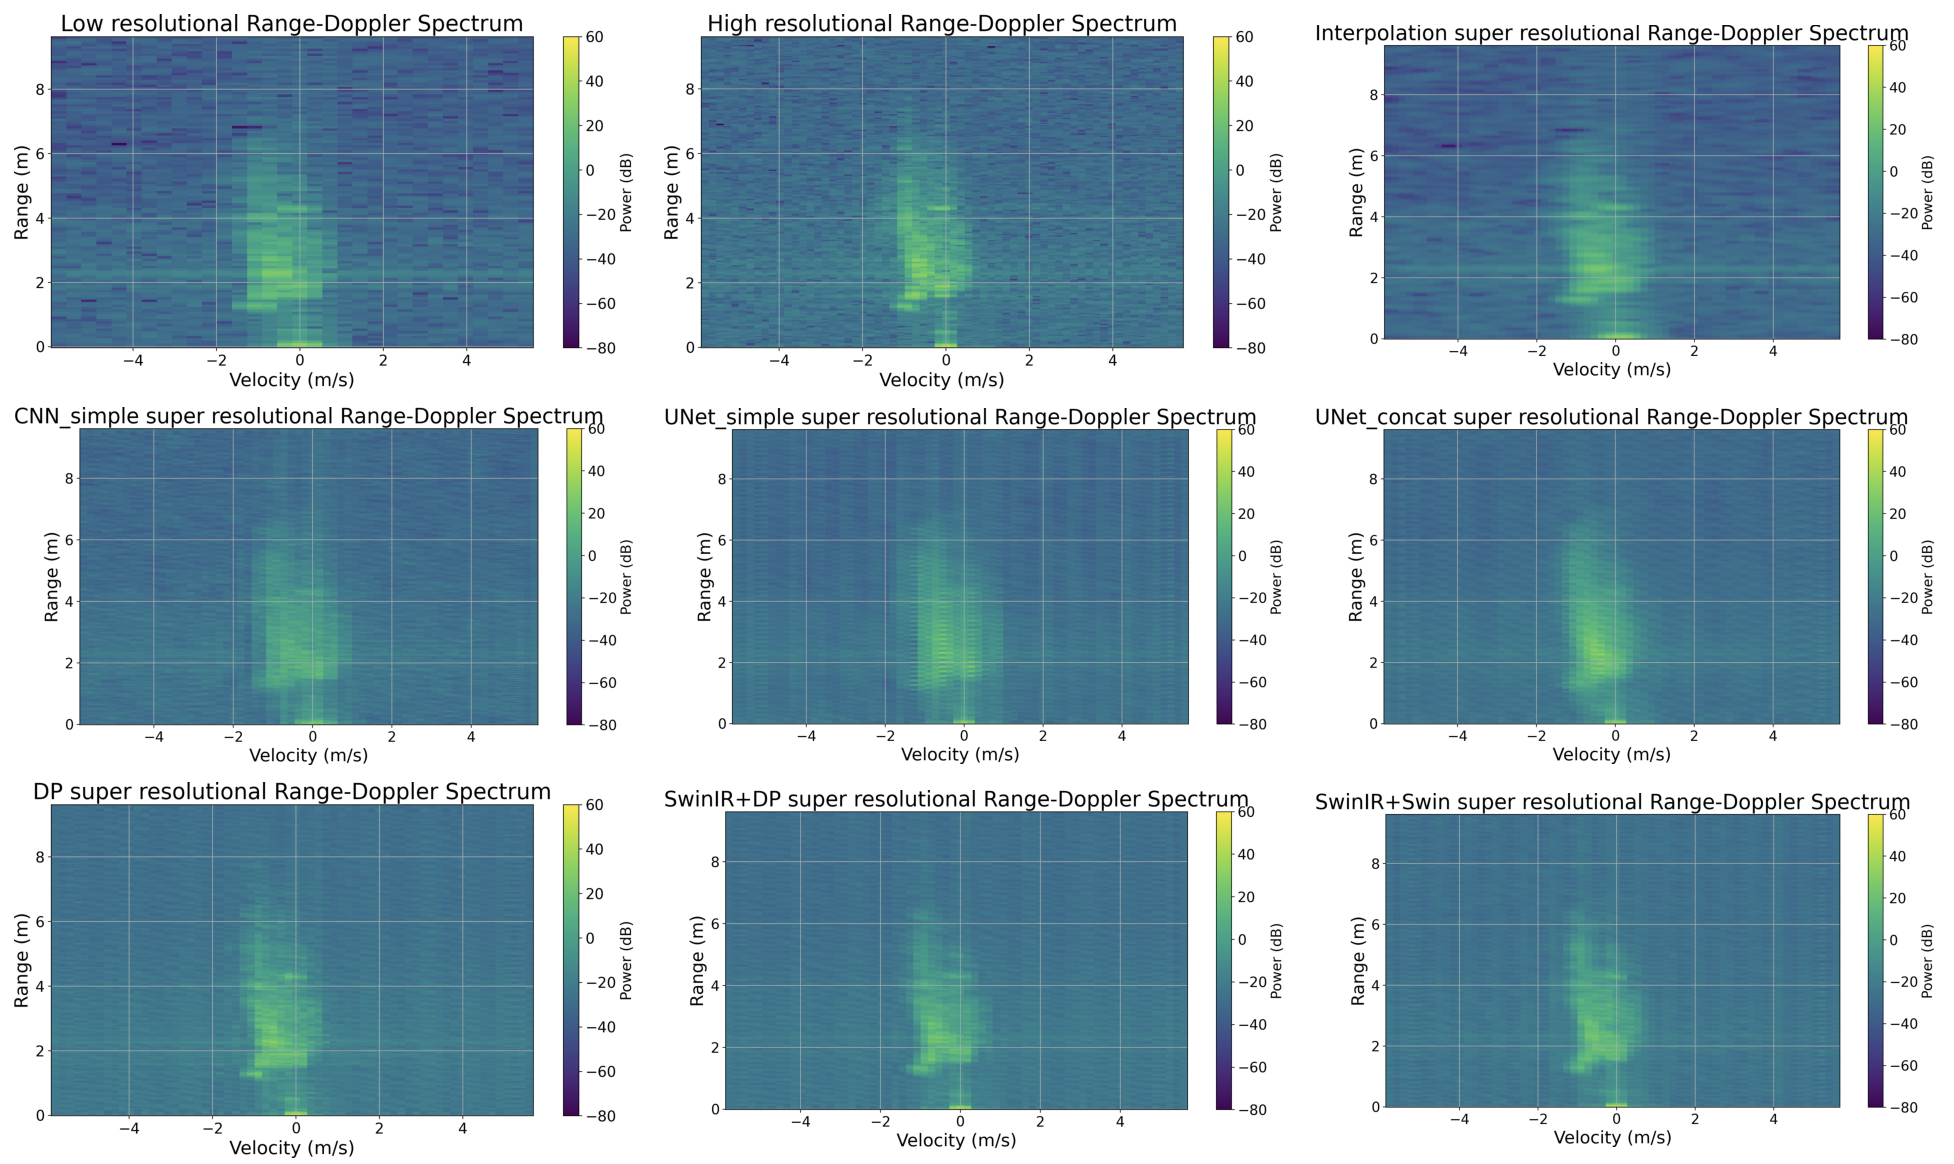
\includegraphics[scale=.45]{thesis/figures/evaluation_models_2.png}
    \caption{Super resolution range-Doppler maps of different models in the case of the loss combination and the new processing methods.}
    \label{evaluation models 2}
\end{figure}

After using the new combination of the processing methods and the loss combination, most of the evaluation losses are optimized. Furthermore, visual effect of the super-resolution range-Doppler map is improved as well. Some peaks in the high-resolution range-Doppler map can be clearly seen in the super-resolution range-Doppler map, especially in the Transformer models. Balanced by the evaluation losses and the visual effect, the \gls{dp}-\gls{tf} Transformer model and \gls{swinir}+\gls{dp} model are still better, where \gls{dp}-\gls{tf} Transformer model performs well in the perceptual loss while \gls{swinir}+\gls{dp} model is good at the other losses. Since the peaks look clearer in \gls{dp}-\gls{tf} Transformer model, following sections will keep using \gls{dp}-\gls{tf} Transformer model.


\section{Processing methods} \label{processing methods comparisons}
Based on the above \gls{dp}-\gls{tf} Transformer model, this section will compare the different combinations of the processing methods, namely input data representation, dimension processing types, upsampling types, logarithm and normalization operations.

\begin{spacing}{1.5}
\textbf{\large{Input data representation}}
\end{spacing}
While processing complex-valued data, there are three types of the input data representation, namely real and imaginary, amplitude as well as amplitude and phase. The other processing methods keep no dimension processing layer, the transposed convolutional upsampling layer, and do not use any logarithm and normalization operations, which means only the representation type is changed compared with the first case in section \ref{models comparisons}. The loss metrics and super-resolution range-Doppler map are shown in Table \ref{Evaluation losses of the separation types comparison} and Figure \ref{Super-resolution images of the separation types} respectively.

\begin{table}
    \centering
    \caption{Evaluation losses of different types of the input data representation, where A1 represents the real and imaginary representation, A2 is the amplitude representation and A3 denotes the amplitude and phase representation.}
    \label{Evaluation losses of the separation types comparison}
    \begin{tabular}{l|c|c|c|c|c}
        \hline
        Representation types & MSE & SDR & LSD & WMSE & Perceptual \\
        \hline
        A1 & 3.435 & -4.958 & 0.619 & \textbf{0.155} & 24.682 \\
        \hline
        A2 & \textbf{3.136} & \textbf{-7.778} & \textbf{0.385} & 0.181 & \textbf{18.101} \\
        \hline
        A3 & 3.213 & -5.068 & 0.493 & 0.241 & 20.126 \\
        \hline
    \end{tabular}
\end{table}

\begin{figure}
    \centering
    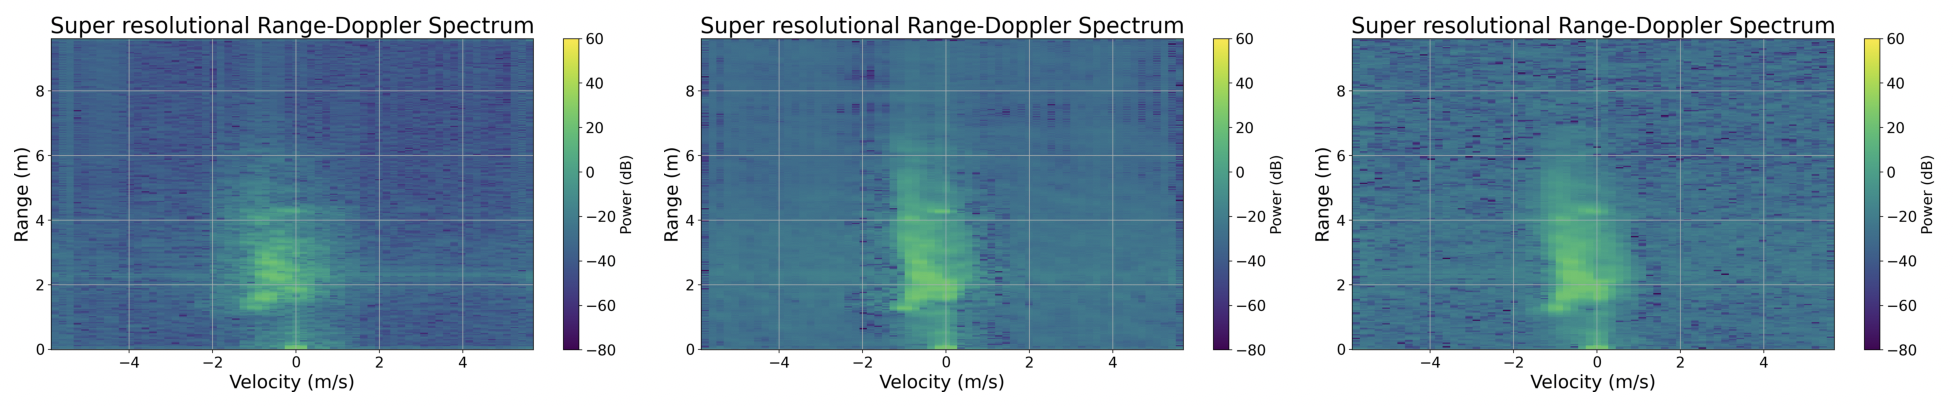
\includegraphics[scale=.45]{figures/evaluation_processing_mse_A.png}
    \caption{Super-resolution range-Doppler maps of different types of the input data representation, from left to right real and imaginary representation, amplitude representation as well as amplitude and phase representation, respectively.}
    \label{Super-resolution images of the separation types}
\end{figure}

Analyzed from the results, since the visualization of range-Doppler map is affected by amplitude, it is beneficial to use amplitude for training. From the perspective of evaluation losses, training with only amplitude is the best. However, since it loses the information of phase, and the amplitude and phase representation type is mostly better than real and imaginary representation type in terms of the evaluation losses and visual effect, the amplitude and phase representation type will be maintained in the subsequent evaluations.

\begin{spacing}{1.5}
\textbf{\large{Dimension processing types}}
\end{spacing}
Operated by the \gls{rfft}, the shape along the range axis turns to an prime value, which will affect both the Transformer division and the downsampling process. However, since there is no downsampling operation and segmentation along the axes in the \gls{dp}-\gls{tf} Transformer model, it can still run normally without additional dimension processing. Therefore, there are three dimensional processing types: no processing, padding, and convolution. Based on the amplitude and phase representation type and keeping other settings unchanged, the loss metrics in Table \ref{Evaluation losses of the dimension processing types comparison} and the super-resolution range-Doppler maps in Figure \ref{super-resolution images of the dimension processing types} are obtained.

\begin{table}
    \centering
    \caption{Evaluation losses of different dimension processing types, where B1 represents no processing type, B2 is the padding and B3 denotes the convolutional layer as the processing type.}
    \label{Evaluation losses of the dimension processing types comparison}
    \begin{tabular}{l|c|c|c|c|c}
        \hline
        Dimension processing & MSE & SDR & LSD & WMSE & Perceptual \\
        \hline
        B1 & 3.100 & -6.312 & 0.427 & 0.194 & 19.081 \\
        \hline
        B2 & 3.113 & \textbf{-6.611} & \textbf{0.420} & \textbf{0.190} & 19.092 \\
        \hline
        B3 & \textbf{2.349} & -5.908 & 0.451 & 0.206 & \textbf{16.259} \\
        \hline
    \end{tabular}
\end{table}

\begin{figure}
    \centering
    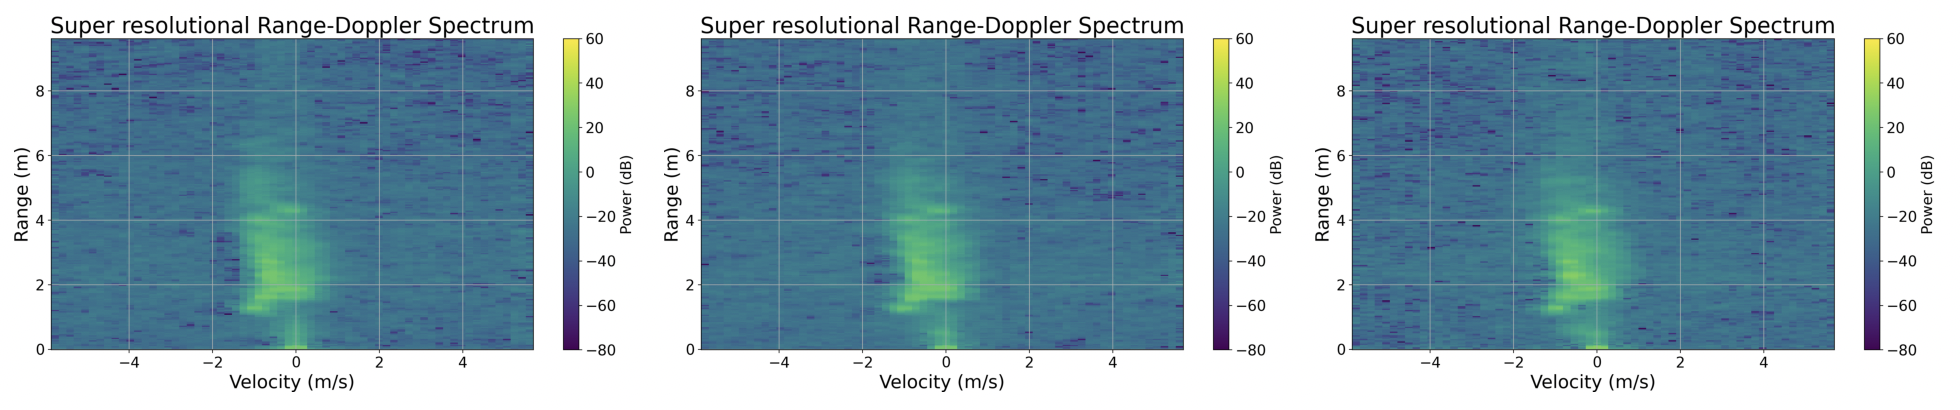
\includegraphics[scale=.45]{figures/evaluation_processing_mse_B.png}
    \caption{Super-resolution range-Doppler maps of different dimension processing types, from left to right no processing, padding and convolution layer, respectively}
    \label{super-resolution images of the dimension processing types}
\end{figure}

While the convolutional layer as the dimension processing type leads to more parameters, the padding processing type can still obtain a better result in multiple evaluation losses. The reason could be that using convolution layer to remove a dimension along the range axis may result in information loss. Subsequent evaluations will be based on the padding dimension processing type.

\begin{spacing}{1.5}
\textbf{\large{Upsampling types}}
\end{spacing}
The two most common upsampling methods are transposed convolutional layer and pixel shuffle approach. The block, containing transposed convolutional layer, \gls{ln} and \gls{relu} activation function, will result in a lot of new parameters, while the pixel shuffle operation does not generate any new parameters. Table \ref{Evaluation losses of the upsampling types comparison} and Figure \ref{super-resolution images of the upsampling types} show the performance of two approaches in terms of evaluation losses and super-resolution range-Doppler maps.

Although the transposed convolutional layer brings a large number of new parameters, it does not surpass pixel shuffle layer in all loss metrics, especially the perceptual loss is higher. Visually, the right range-Doppler map in Figure \ref{super-resolution images of the upsampling types} is even more reasonable for the dynamic range part. Therefore, the pixel shuffle layer will be used as the upsampling type in the subsequent evaluations.

\begin{table}
    \centering
    \caption{Evaluation losses of different upsampling types, where C1 represents the transposed convolutional layer and C2 denotes the pixel shuffle approach as the upsampling layer.}
    \label{Evaluation losses of the upsampling types comparison}
    \begin{tabular}{l|c|c|c|c|c|c}
        \hline
        Upsampling types & \#Params & MSE & SDR & LSD & WMSE & Perceptual \\
        \hline
        C1 & 113,866 & 3.113 & \textbf{-6.611} & \textbf{0.420} & \textbf{0.190} & 19.092 \\
        \hline
        C2 & 48,042 & \textbf{2.560} & -4.206 & 0.506 & 0.269 & \textbf{17.918} \\
        \hline
    \end{tabular}
\end{table}

\begin{figure}
    \centering
    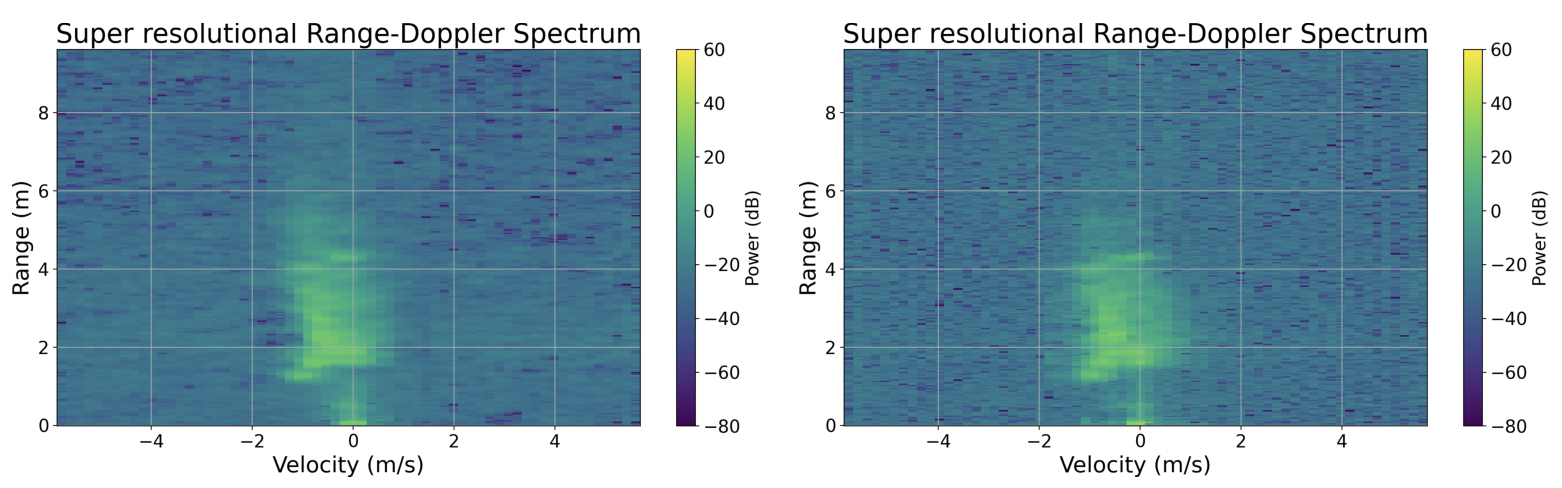
\includegraphics[scale=.45]{thesis/figures/evaluation_processing_C.png}
    \caption{Super-resolution range-Doppler maps of different upsampling types, left using the transposed convolutional layer and right with the pixel shuffle layer.}
    \label{super-resolution images of the upsampling types}
\end{figure}


\begin{spacing}{1.5}
\textbf{\large{Logarithm types}}
\end{spacing}
When the amplitude is part of the input, the range of the amplitude will affect the learning process, causing it to focus more on areas with higher signal power and ignore the loss caused by areas with less amplitude. Therefore, in this evaluation, the impact of the logarithm operation will be evaluated.

\begin{table}
    \centering
    \caption{Evaluation losses of the effect of the logarithm, where D1 represents no logarithm operation, D2 uses the base 10 logarithm operation. Accordingly, the \gls{mse} training loss in D1 case uses the amplitude in linear scale while in D2 uses the logarithmic amplitude.}
    \label{Evaluation losses of the logarithm types comparison}
    \begin{tabular}{l|c|c|c|c|c}
        \hline
        Logarithm types & MSE & SDR & LSD & WMSE & Perceptual \\
        \hline
        D1 & 2.560 & -4.206 & 0.506 & 0.269 & 17.918 \\
        \hline
        D2 & \textbf{1.740} & \textbf{-9.251} & \textbf{0.295} & \textbf{0.130} & \textbf{17.636} \\
        \hline
    \end{tabular}
\end{table}

\begin{figure}
    \centering
    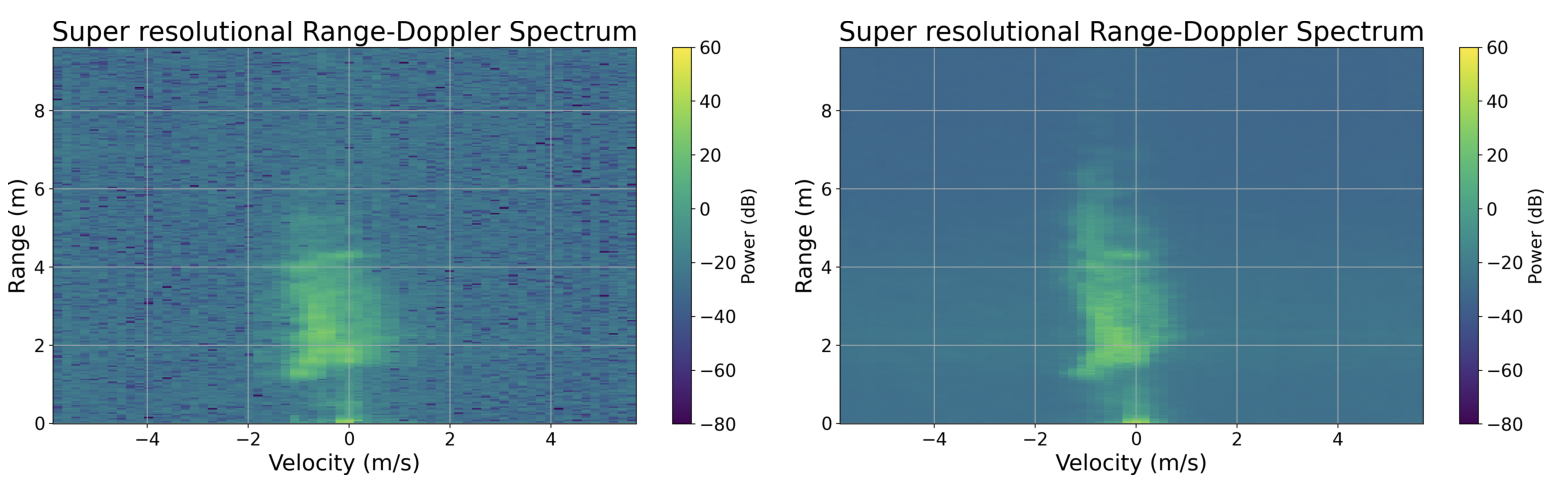
\includegraphics[scale=.45]{figures/evaluation_processing_D.png}
    \caption{Super-resolution range-Doppler maps of the cases without logarithm and with logarithm operation, from left to right, respectively.}
    \label{super-resolution images of the logarithm types}
\end{figure}

From Table \ref{Evaluation losses of the logarithm types comparison}, it can be clearly seen that after using the logarithm operation with base 10, significant improvements have been achieved in all evaluation losses. However, compared with the left range-Doppler map in Figure \ref{super-resolution images of the logarithm types}, the right super-resolution range-Doppler map has a blurring effect in the background. The reason would be that in the left range-Doppler map the model pays less attention on the low amplitude signal as well as the noise and uses smaller values instead. After using the logarithm, the signals with low amplitude get more attention while the noise is still hard to learn, so that the noise is mostly predicted as relatively low amplitude and then look blurry.

\begin{spacing}{1.5}
\textbf{\large{Amplitude normalization types}}
\end{spacing}
Similar to the idea of logarithm operation, the normalization operation can reduce the dynamic range of the data. According to the maximum and minimum values of each dataset, the amplitude of each dataset can be accordingly converted to the range of (-1, 1) or (0, 1) . In addition, it can also be not normalized. Furthermore, since the normalization will result in a small gradient, the learning rate is tuned by the cases, only the case without normalization uses the learning rate as 1e-5, otherwise the learning rate as 1e-3. The results of the evaluation losses and the super-resolution range-Doppler maps are shown in Table \ref{Evaluation losses of the amplitude normalization types comparison in the case of no angle normalization} and Figure \ref{evaluation processing E} respectively.

\begin{table}
    \centering
    \caption{Evaluation losses of different amplitude normalization types, where E1 represent no normalization operation, E2 is in the range of (-1, 1), E3 denotes in the range of (0,1).}
    \label{Evaluation losses of the amplitude normalization types comparison in the case of no angle normalization}
    \begin{tabular}{l|c|c|c|c|c}
        \hline
        Amplitude normalization & MSE & SDR & LSD & WMSE & Perceptual \\
        \hline
        E1 & 1.740 & \textbf{-9.251} & \textbf{0.295} & 0.130 & 17.636 \\
        \hline
        E2 & 1.711 & -6.841 & 0.349 & \textbf{0.108} & 14.770 \\
        \hline
        E3 & \textbf{1.073} & -6.327 & 0.358 & 0.119 & \textbf{14.639} \\
        \hline
    \end{tabular}
\end{table}

\begin{figure}
    \centering
    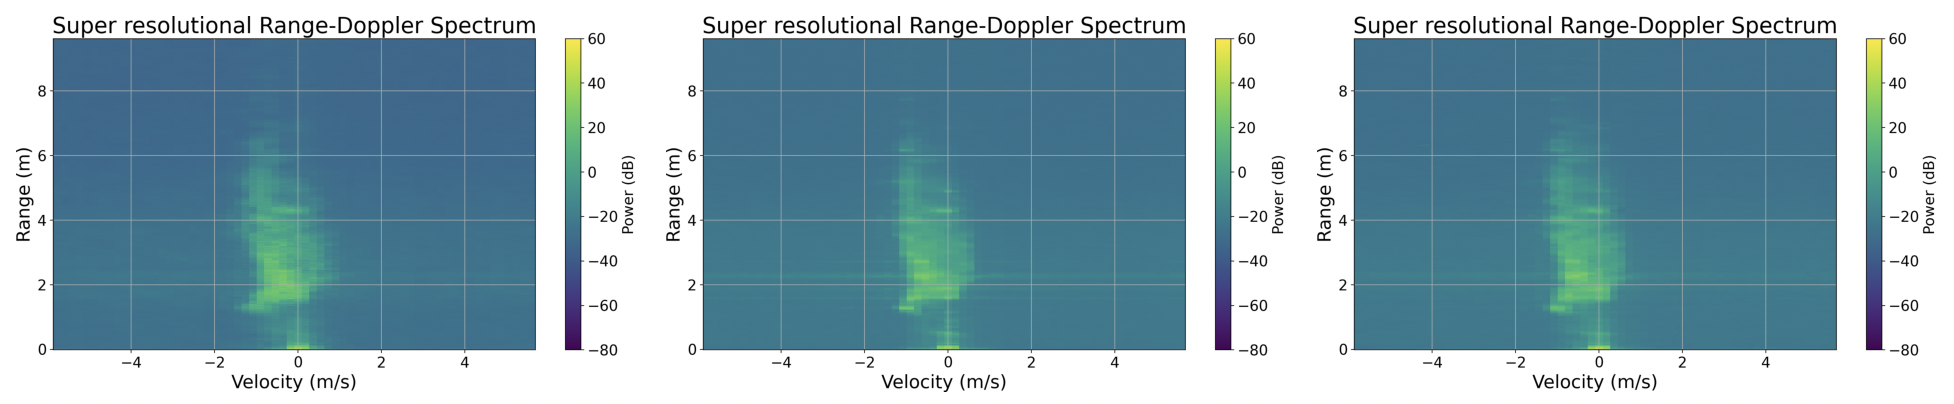
\includegraphics[scale=.45]{figures/evaluation_processing_E.png}
    \caption{Super-resolution range-Doppler maps of different amplitude normalization types, from left to right, no amplitude normalization, normalization in (-1, 1) and normalization in (0, 1), respectively.}
    \label{evaluation processing E}
\end{figure}

In general, the introduction of the normalization operation is conducive to reduce multiple evaluation losses, among which the optimization of perceptual loss is the most obvious, which represents visual optimization, since the \gls{vgg} expects the normalized input, ideally in the (0, 1) range. The normalization in (0, 1) form obtains the most balanced result, so the amplitude normalization will be kept in the range of (0, 1) in subsequent evaluations.

\begin{spacing}{1.5}
\textbf{\large{Angle normalization types}}
\end{spacing}
In the amplitude and phase representation type, in addition to the amplitude being normalized, the angle can also be normalized and converted to (-1, 1) divided by  $\mathrm{\pi}$. The results are shown in Table \ref{Evaluation losses of the angle normalization types comparison} and Figure \ref{evaluation processing F}.

From the results, the normalization of the angle doesn't bring much improvement in the most evaluation losses. The reason is that the angle itself is within the range of (-$\mathrm{\pi}$, $\mathrm{\pi}$), and its dynamic range is not that large as amplitude. Therefore, the normalization operation will not cause many differences.

\begin{table}
    \centering
    \caption{Evaluation losses of the effect of the angle normalization type, where F1 represent no angle normalization operation, F2 denotes the angle normalization in the range of (-1, 1).}
    \label{Evaluation losses of the angle normalization types comparison}
    \begin{tabular}{l|c|c|c|c|c}
        \hline
        Angle normalization & MSE & SDR & LSD & WMSE & Perceptual \\
        \hline
        F1 & \textbf{1.073} & \textbf{-6.327} & \textbf{0.358} & 0.119 & \textbf{14.639} \\
        \hline
        % F2 & 1.154 & \textbf{-6.814} & \textbf{0.349} & \textbf{0.115} & \textbf{14.607} \\
        % \hline
        F2 & 1.330 & -6.068 & 0.363 & \textbf{0.117} & 15.204 \\
        \hline
    \end{tabular}
\end{table}

\begin{figure}
    \centering
    \includegraphics[scale=.45]{thesis/figures/evaluation_processing_F_new.png}
    \caption{Super-resolution range-Doppler maps of the effect of the angle normalization type, left without angle normalization and right with angle normalization.}
    \label{evaluation processing F}
\end{figure}

In conclusion, based on the above evaluations and analysis, the combination of processing methods tends to use padding for dimensional processing, pixel shuffle approach as the upsampling type, amplitude and phase representation determined as the conversion of the complex-valued data, logarithm operation and normalization operation in the range of (0, 1) on the amplitude, but no additional normalization operation performed on the phase.

\section{Training loss functions} \label{training loss functions evaluations}
Different from the evaluation loss functions, there are six types of training loss functions. Based on the optimal combination of the processing methods combination obtained in the section \ref{processing methods comparisons} and \gls{dp}-\gls{tf} Transformer model, different training loss functions are used to train the model, so as to obtain one training loss function that is most suitable for the range-Doppler map upsampling task. The hyperparameters such as the ratio $\lambda$ between the amplitude loss and angle loss in the training loss function and learning rate will be adjusted according to their values according to a few batches at the very beginning. In addition, \gls{sdr} and perceptual loss functions require a pretraining phase by the \gls{lsd} training loss function, since they are not stable in the early stage. Table \ref{Evaluation losses of the training loss functions comparison} and Figure \ref{training loss functions comparison} are the results obtained by different training loss functions.


\begin{table}
    \centering
    \caption{Evaluation losses of different training loss functions, horizontal axis is the evaluation loss functions, vertical axis is the training loss functions.}
    \label{Evaluation losses of the training loss functions comparison}
    \begin{tabular}{l|c|c|c|c|c}
        \hline
        Loss comparison & MSE & SDR & LSD & WMSE & Perceptual \\
        \hline
        MSE & \textbf{1.073} & -6.327 & 0.358 & 0.119 & 14.639 \\
        \hline
        SDR & 1.110 & -5.683 & 0.370 & 0.121 & 14.163 \\
        \hline
        LSD & 1.232 & \textbf{-6.736} & \textbf{0.351} & \textbf{0.108} & 14.198 \\
        \hline
        PLSD & 1.424 & -6.434 & 0.356 & 0.124 & 16.999 \\
        \hline
        WMSE & 1.279 & -5.967 & 0.365 & 0.131 & 17.478 \\
        \hline
        Perceptual & 6.174 & -4.129 & 0.417 & 0.393 & \textbf{13.882} \\
        \hline
    \end{tabular}
\end{table}

\begin{figure}
    \centering
    \includegraphics[scale=.4]{thesis/figures/evaluation_loss_functions.png}
    \caption{Super-resolution range-Doppler maps of different training loss functions, in the first row from left to right MSE, SDR and LSD, in the second row from left to right PLSD, WMSE and perceptual loss functions.}
    \label{training loss functions comparison}
\end{figure}

From the results, it can be seen that the \gls{lsd} training loss function can obtain better results in most of the evaluation losses, but from the visual perspective of super-resolution range-Doppler maps, the range-Doppler maps trained by perceptual loss effectively eliminate the blurring problem, that is, the amplitude difference in the background can be seen. Therefore, the training loss function \gls{lsd} can be combined with the perceptual loss to take advantage of both pros.

\begin{spacing}{1.5}
\textbf{\large{Loss combination}}
\end{spacing} 
According to the loss combination as written in formula \ref{loss combination equation}, the relationship $\lambda_c$ between \gls{lsd} and perceptual loss should be determined. We compare a few loss values of the early batches and make sure that the main loss value comes from the \gls{lsd} loss but still influenced by the perceptual loss to a certain content, then Table \ref{Evaluation losses of the training loss functions combination comparison} and Figure \ref{lsd+perceptual combination} are obtained.

\begin{table}
    \centering
    \caption{Evaluation losses of the training loss combination with different ratios.}
    \label{Evaluation losses of the training loss functions combination comparison}
    \begin{tabular}{l|c|c|c|c|c}
        \hline
        LSD combination & MSE & SDR & LSD & WMSE & Perceptual \\
        \hline
        Lambda=1 & 2.464 & -5.270 & 0.383 & 0.220 & 13.779 \\
        \hline
        Lambda=0.5 & 1.731 & -5.375 & 0.380 & 0.179 & \textbf{12.320 }\\
        \hline
        Lambda=1e-1 & 1.347 & -5.829 & 0.369 & 1.150 & 12.979 \\
        \hline
        Lambda=1e-2 & 1.288 & -6.514 & 0.355 & 0.116 & 13.213 \\
        \hline
        Lambda=1e-3 & 1.486 & \textbf{-7.268} & \textbf{0.341} & \textbf{0.108} & 13.729 \\
        \hline
        Lambda=1e-4 & \textbf{1.265} & -6.405 & 0.357 & 0.115 & 14.138 \\
        \hline
    \end{tabular}
\end{table}

\begin{figure}
    \centering
    \includegraphics[scale=.45]{figures/evaluation_loss_combination.png}
    \caption{Super-resolution range-Doppler maps of the training loss combination with different ratios, in the first row from left to right are lambda as 1, 0.5 and 0.1, while in the second row from left to right 1e-2, 1e-3, 1e-4.}
    \label{lsd+perceptual combination}
\end{figure}

The overall relationship between the \gls{lsd} loss function and perceptual loss function is that with the importance of the perceptual loss increasing in the loss combination, the evaluation perceptual loss decreases while the other evaluation losses is increasing. Since the loss combination is going to optimize the perceptual loss, the hyperparameter $\lambda_C$ is determined as 0.5, that is, the training loss function written as
\begin{equation}
    \centering
    \mathcal{L}_{\text{Combination}} = \mathcal{L}_{\text{LSD}} + 0.5 \times \mathcal{L}_{\text{Perceptual}}.
    \label{loss combination}
\end{equation}


\section{cGAN comparison} \label{cGAN comparison}
With the mutual supervision of the generator and discriminator, the output of generator can be visually more pleasing. Therefore, in this section, the \gls{cgan} model is evaluated, the generator keeps using the \gls{dp}-\gls{tf} Transformer model, and target training loss function is the loss combination from section \ref{training loss functions evaluations}. The generator loss is denoted as
\begin{equation}
    \centering
    \mathcal{L}_{\text{Gen}} = \mathcal{L}_{\text{LSD}} + 0.5 \times \mathcal{L}_{\text{Perceptual}} + \lambda_g \times \mathcal{L}_{\text{GAN, Gen}},
    \label{loss combination}
\end{equation}

where $\lambda_g$ is going to be tuned. Furthermore, as said in section \ref{discriminator}, the discriminator has two types, no low-resolution range-Doppler maps or with low-resolution range-Doppler maps as input. Therefore, both cases have been evaluated, where Table \ref{Evaluation losses of the cGAN model comparison in the case of discriminator without low-resolution image as input} and Figure \ref{Super-resolution images of the cGAN model no low-res} show the results in the case of the discriminator without any low-resolution information while Table \ref{Evaluation losses of the cGAN model comparison in the case of discriminator with low-resolution image as input} and Figure \ref{Super-resolution images of the cGAN model with low-res} are the results given the low-resolution range-Doppler maps.

\begin{table}
    \centering
    \caption{Evaluation losses of the adversarial loss combination with different ratios in the case of the discriminator without low-resolution range-Doppler maps as input.}
    \label{Evaluation losses of the cGAN model comparison in the case of discriminator without low-resolution image as input}
    \begin{tabular}{l|c|c|c|c|c}
        \hline
        cGAN & MSE & SDR & LSD & WMSE & Perceptual \\
        \hline
        $\lambda_g$=5e-1 & 1.802 & -5.216 & 0.383 & 0.186 & 13.543 \\
        \hline
        $\lambda_g$=1e-1 & 1.621 & -5.183 & 0.384 & 0.172 & 12.898 \\
        \hline
        $\lambda_g$=5e-2 & \textbf{1.447} & -5.463 & 0.379 & 0.181 & 13.311 \\
        \hline
        $\lambda_g$=1e-2 & 1.640 & -5.690 & 0.374 & \textbf{0.169} & \textbf{11.881} \\
        \hline
        $\lambda_g$=5e-3 & 1.525 & -5.305 & 0.382 & 0.193 & 12.956 \\
        \hline
        $\lambda_g$=1e-3 & 2.072 & \textbf{-5.845} & \textbf{0.370} & 0.182 & 14.396 \\
        \hline
    \end{tabular}
\end{table}

\begin{figure}
    \centering
    \includegraphics[scale=.45]{thesis/figures/evaluation_cGAN_no_low_res.png}
    \caption{Super-resolution range-Doppler maps of the adversarial loss combination with different ratios in the case of the discriminator without low-resolution range-Doppler maps as input, in the first row from left to right are $\lambda_g$ as 5e-1, 1e-1 and 5e-2, while in the second row from left to right 1e-2, 5e-3, 1e-3.}
    \label{Super-resolution images of the cGAN model no low-res}
\end{figure}

It can be seen that \gls{cgan} model is able to improve the perceptual loss, no matter with or without the low-resolution range-Doppler map. Both cases are better, especially when the adversarial loss ratio sets as 1e-2, whereas the discriminator without the low-resolution range-Doppler map gets a relatively better perceptual evaluation loss. The reason could be that the concatenating operation of the low-resolution and high(super)-resolution range-Doppler map would confuse the discriminator, that is, the discriminator focuses more on the mapping relationship between low- and super-resolution range-Doppler map, rather than on the super-resolution range-Doppler map itself, and additionally, the loss calculation in the perceptual loss has no inputs of the low-resolution range-Doppler map. Perhaps the comparison directly between the super- and high-resolution range-Doppler maps is simple for the discriminator rather than with the low-resolution range-Doppler map as the medium. In conclusion, the discriminator without low-resolution range-Doppler map will be used and the generator loss turns to be

\begin{equation}
    \centering
    \mathcal{L}_{\text{Gen}} = \mathcal{L}_{\text{LSD}} + 0.5 \times \mathcal{L}_{\text{Perceptual}} + 0.01 \times \mathcal{L}_{\text{GAN, Gen}}.
    \label{loss combination}
\end{equation}


\begin{table}[!htp]
    \centering
    \caption{Evaluation losses of the adversarial loss combination with different ratios in the case of the discriminator with low-resolution range-Doppler maps as input, where the number of parameters of the generator is 48,042 while that of the discriminator is 76,267.}
    \label{Evaluation losses of the cGAN model comparison in the case of discriminator with low-resolution image as input}
    \begin{tabular}{l|c|c|c|c|c}
        \hline
        cGAN & MSE & SDR & LSD & WMSE & Perceptual \\
        \hline
        $\lambda_g$=1e-1 & 1.592 & -5.361 & 0.381 & 0.164 & 13.861 \\
        \hline
        $\lambda_g$=5e-2 & 1.491 & -5.628 & \textbf{0.374} & \textbf{0.158} & 12.126 \\
        \hline
        $\lambda_g$=1e-2 & \textbf{1.339} & -5.103 & 0.385 & 0.177 & \textbf{11.926} \\
        \hline
        $\lambda_g$=5e-3 & 1.628 & -5.461 & 0.379 & 0.165 & 13.511 \\
        \hline
        $\lambda_g$=1e-3 & 1.920 & \textbf{-5.648} & 0.375 & 0.159 & 13.257 \\
        \hline
        $\lambda_g$=1e-4 & 3.593 & -5.331 & 0.381 & 0.190 & 14.148 \\
        \hline
    \end{tabular}
\end{table}

\begin{figure}[!htp]
    \centering
    \includegraphics[scale=.45]{thesis/figures/evaluation_cGAN_with_low_res.png}
    \caption{Super-resolution range-Doppler maps of the adversarial loss combination with different ratios in the case of the discriminator with low-resolution range-Doppler maps as input, in the first row from left to right are $\lambda_g$ as 1e-1, 5e-2 and 1e-2, while in the second row from left to right 5e-3, 1e-3 and 1e-4.}
    \label{Super-resolution images of the cGAN model with low-res}
\end{figure}


\section{VGG layers in the perceptual loss} \label{vgg layers comparison}
In this section, different combinations of the \gls{vgg} layers are evaluated, by default the last convolutional layers of the first four blocks are used. Table \ref{Evaluation losses of different VGG layers} and Figure \ref{Super-resolution images of different VGG layers} show the results trained by the loss combination with different \gls{vgg} layers used. With the deeper layer to be used, many evaluation losses decrease. However, in order to improve the perceptual loss, the default combination is still better one.

\begin{table}[!htp]
    \centering
    \caption{Evaluation losses of different combinations of the VGG layers in the training loss combination.}
    \label{Evaluation losses of different VGG layers}
    \begin{tabular}{l|c|c|c|c|c}
        \hline
        VGG layers comparison & MSE & SDR & LSD & WMSE & Perceptual \\
        \hline
        b1c2+b2c2+b3c4 & 1.975 & -5.366 & 0.380 & 0.167 & 12.793 \\
        \hline
        b1c2+b2c2+b3c4+b4c4 & 1.731 & -5.375 & 0.380 & 0.179 & \textbf{12.320} \\
        \hline
        b1c2+b2c2+b3c4+b4c4+b5c4 & 1.731 & \textbf{-6.082} & \textbf{0.366} & \textbf{0.157} & 13.714 \\
        \hline
        b2c2+b3c4+b4c4 & \textbf{1.730} & -5.530 & 0.379 & 0.186 & 14.857 \\
        \hline
    \end{tabular}
\end{table}

\begin{figure}[!htp]
    \centering
    \includegraphics[scale=.45]{thesis/figures/evaluation_vgg.png}
    \caption{Super-resolution range-Doppler maps of different combinations of the VGG layers in the training loss combination, in the first row from left to right as b1c2+b2c2+b3c4 and b1c2+b2c2+b3c4+b4c4, in the second row as b1c2+b2c2+b3c4+b4c4+b5c4 and b2c2+b3c4+b4c4.}
    \label{Super-resolution images of different VGG layers}
\end{figure}


\section{Number of frames} \label{FOL comparison}
Since the range-Doppler map is always collected dynamically, that is, the continuous frames will have some relationship and the model could get more motion information. In this thesis, everything discussed previously is based on the setting that the number of frames in the inputs is 4. In this section, the effects of different numbers of frames values on the model will be evaluated. Table \ref{Evaluation losses of FOL comparison} and Figure \ref{Super-resolution images of different FOL values} illustrate the difference between the two cases.

From the evaluation losses from different cases, when the number of frames is chosen as 4, it can achieve a better result. Therefore, the continuous motion information is useful for the model and it verifies the previous assumption as well.

\begin{table}[!htp]
    \centering
    \caption{Evaluation losses of different numbers of frames values.}
    \label{Evaluation losses of FOL comparison}
    \begin{tabular}{l|c|c|c|c|c}
        \hline
        \#Frames comparison & MSE & SDR & LSD & WMSE & Perceptual \\
        \hline
        \multicolumn{6}{c}{\textbf{\#Frames = 1}}\\
        \hline
        DP & \textbf{1.379} & -5.239 & 0.381 & 0.191 & 12.778 \\
        \hline
        cGAN & 1.950 & -3.930 & 0.409 & 0.236 & 13.063 \\
        \hline
        \multicolumn{6}{c}{\textbf{\#Frames = 4}}\\
        \hline
        DP & 1.731 & \textbf{-5.375} & \textbf{0.380} & \textbf{0.179} & \textbf{12.320} \\
        \hline
        cGAN & \textbf{1.640} & \textbf{-5.690} & \textbf{0.374} & \textbf{0.169} & \textbf{11.881} \\
        \hline
    \end{tabular}
\end{table}

\begin{figure}[!htp]
    \centering
    \begin{subfigure}{0.95\textwidth}
        \centering
        \includegraphics[width=\textwidth]{thesis/figures/evaluation_FOL1.png}
        \caption{Super-resolution range-Doppler maps with one frame as input, where in the second row the left from DP-TF Transformer model and the right from cGAN model.}
        \label{Super-resolution image while FOL value as 1}
    \end{subfigure}
    \vspace{0.3cm}
    \begin{subfigure}{0.95\textwidth}
        \centering
        \includegraphics[width=\textwidth]{thesis/figures/evaluation_FOL4_under.png}
        \caption{Super-resolution range-Doppler maps with four frames as input, where the left from DP-TF Transformer model and the right from cGAN model.}
        \label{Super-resolution image while FOL value as 4}
    \end{subfigure}
    \caption{Super-resolution range-Doppler maps of different numbers of frames}
    \label{Super-resolution images of different FOL values}
\end{figure}

\section{Resampling rate} \label{Resampling rate comparison}
With the optimal processing methods and loss combination, the case that the 4$\times$ downsampled low-resolution range-Doppler map is evaluated with both \gls{dp}-\gls{tf} Transformer model and \gls{cgan} model in this section. Table \ref{Evaluation losses while the resampling rate as 4} and Figure \ref{Super-resolution images while the resampling rate as 4} show the results. However, the evaluation losses as well as the super-resolution range-Doppler maps look not as good as the case of 2$\times$ downsampled low-resolution range-Doppler map. The reason is that too much information is lost, only the shape of the part with high signal power can be seen.

\begin{table}[!htp]
    \centering
    \caption{Evaluation losses while the resampling rate as 4.}
    \label{Evaluation losses while the resampling rate as 4}
    \begin{tabular}{l|c|c|c|c|c}
        \hline
        Resampling rate & MSE & SDR & LSD & WMSE & Perceptual \\
        \hline
        DP & 2.208 & 5.811 & 0.620 & 0.491 & 22.347 \\
        \hline
        cGAN & 2.307 & 5.166 & 0.600 & 0.429 & 22.162 \\
        \hline
    \end{tabular}
\end{table}

\begin{figure}[!htp]
    \centering
    \includegraphics[scale=.45]{thesis/figures/evaluation_resampling4.png}
    \caption{Super-resolution range-Doppler maps while the resampling rate as 4, where in the second row the left from DP-TF Transformer model and the right from cGAN model.}
    \label{Super-resolution images while the resampling rate as 4}
\end{figure}

\section{Distributed training speed} \label{Distributed training evaluation}
To speed up the training process, the distributed training is used in the pipeline. The speed comparison is illustrated in Figure \ref{Evaluation of the speed by the distributed training}, which is recorded as the distributed training was successfully implemented, where \gls{dp}-\gls{tf} Transformer model is used in a large scale. The time taken in each epoch decreases from roughly 1800 seconds to under 400 seconds, that is, it uses multiple \gls{gpu}s successfully.


\begin{figure}[!htp]
    \centering
    \includegraphics[scale=.45]{thesis/figures/evaluation_distributed_training.png}
    \caption{Evaluation of the speed by the distributed training, where the red line represents the pipeline without distributed training while cyan line with.}
    \label{Evaluation of the speed by the distributed training}
\end{figure}


\section{Hyperparameters tuning} \label{hyperparameters tuning evaluation}
The hyperparameters of the model and training process have an impact on the result, such as the number of blocks, the number of filters, etc. Therefore, in this section, the sweep function in \gls{wandb} is used to combine and evaluate some hyperparameters to find a better combination that minimizes the loss. Figure \ref{Hyperparameters tuning by WandB} shows the sweep process of \gls{wandb}. With optimal combination of the hyperparameters, the evaluation losses and the visual effect of the super-resolution range-Doppler maps have improved as shown in Table \ref{Evaluation losses after hyperparameters tuning} and Figure \ref{Super-resolution images after the hyperparameters tuning}.

\begin{figure}[!htp]
    \centering
    \includegraphics[scale=.54]{thesis/figures/evaluation_hyperparameters_tuning.png}
    \caption{Hyperparameter tuning by WandB}
    \label{Hyperparameters tuning by WandB}
\end{figure}

\begin{table}[!htp]
    \centering
    \caption{Evaluation losses after hyperparameters tuning}
    \label{Evaluation losses after hyperparameters tuning}
    \begin{tabular}{l|c|c|c|c|c}
        \hline
        Hyperparameters tuning & MSE & SDR & LSD & WMSE & Perceptual \\
        \hline
        DP & 1.225 & -5.625 & 0.373 & 0.146 & 11.753 \\
        \hline
        cGAN & 1.223 & -5.187 & 0.382 & 0.157 & 10.915 \\
        \hline
    \end{tabular}
\end{table}

\begin{figure}[!htp]
    \centering
    \includegraphics[scale=.4]{thesis/figures/evaluation_tune.png}
    \caption{Super-resolution range-Doppler maps after the hyperparameters tuning, in the second row left on trained by DP-TF Transformer model while right one trained by cGAN model.}
    \label{Super-resolution images after the hyperparameters tuning}
\end{figure}


\section{Final result} \label{final result evaluation}
Keeping the same tuned hyperparameters as evaluated in section \ref{hyperparameters tuning evaluation}, after running more epochs with the large model as well as the whole dataset, the evaluation losses and super-resolution range-Doppler maps are further improved as shown in Table \ref{Evaluation losses with large models and whole dataset} and Figure \ref{Super-resolution images trained by large models and whole dataset}.
% The reason about the perceptual loss from \gls{cgan} model no longer smaller than \gls{dp}-\gls{tf} Transformer model would be that the scale of the discriminator is not large enough, when the large generator and the whole dataset are used, the generator improves a lot while the limit of the discriminator is reached.

\begin{table}[!htp]
    \centering
    \caption{Evaluation losses with large models and whole dataset, where the number of parameters of the DP-TF Transformer model and the generator is 329,410 while that of the discriminator is still 766,187.}
    \label{Evaluation losses with large models and whole dataset}
    \begin{tabular}{l|c|c|c|c|c}
        \hline
        Final result & MSE & SDR & LSD & WMSE & Perceptual \\
        \hline
        DP & 0.968 & -6.008 & 0.363 & 0.123 & 9.079 \\
        \hline
        cGAN & 0.803 & -5.619 & 0.371 & 0.120 & 8.740 \\
        \hline
    \end{tabular}
\end{table}

\begin{figure}[!htp]
    \centering
    \includegraphics[scale=.4]{thesis/figures/evaluation_large_new.png}
    \caption{Super-resolution range-Doppler maps trained by large models and whole dataset, in the second row left one trained by DP-TF Transformer model while right one trained by cGAN model.}
    \label{Super-resolution images trained by large models and whole dataset}
\end{figure}

\chapter{Summary \& Outlook} \label{summary and outlook}
This chapter summarizes the results and improvements of the range-Doppler map upsampling task and give an outlook on the future research.

\section{Summary} \label{summary}
In summary, the thesis uses the combination of multiple data processing methods, models, and loss functions to upsample the range-Doppler map with lower resolution. The range-Doppler map is collected in the indoor environment, that is, it has more information and the dynamic range of the amplitude is wide, which poses the high requirement on the training process. However, through a series of optimizations, the final result is significantly improved compared to the general image upsampling approaches.

Firstly, the motivation of this task is introduced. Although chirp sequence radar can achieve high resolution, it cannot achieve the ideal resolution in practice due to the influence of the whole system or regulation. However, the range-Doppler map is an important part of the subsequent positioning and other operations, so a super-resolution one is needed. Meanwhile, we introduce some state-of-the-art upsampling models and papers.

Since the collection scenarios of many public datasets about the range-Doppler map are not sufficient to cope with complex environment, we choose to collect them by ourselves. Using the radar device of Infineon to dynamically collect data in the corridor, the range-Doppler map will contain both range and velocity information, and can ensure the complexity. Furthermore, by loading the data into the \gls{tfrecord} files to speed up the training process, the data is also processed, such as downsampling, loading it with the certain number of frames, and converting it from the time domain to the frequency domain using \gls{rdp}. Moreover, three methods for preprocessing the data are introduced, namely the input data representation on the complex-valued data in frequency domain, logarithm and normalization operation. According to the comparison and evaluation in section \ref{processing methods comparisons}, we choose the amplitude and phase representation type, logarithm and normalization operations in the range of (0, 1) on the amplitude, but no additional operations are performed on the phase. The resolution and maximum values of the range and velocity are derived as well, which are necessary for the visualization of the range-Doppler map.

According to the image upsampling models in the state of the art introduced above, we built seven models, namely the basic \gls{cnn} model, the basic UNet model, the UNet model with concatenating structure, three Transformer models according to different data division methods, and the \gls{cgan} model. Through the two times comparisons in section \ref{models comparisons}, the \gls{dp}-\gls{tf} Transformer model and SwinIR+DP model look better in evaluation loss and super-resolution range-Doppler maps, especially the \gls{dp}-\gls{tf} Transformer model. The reason is that division along the dimensions of range and velocity is conducive for the Transformer model to better learn the relationship between them. In addition, affected by \gls{rdp}, there are prime numbers in the range dimension, so a variety of processing methods are introduced, among which the padding method was determined according to the evaluation in section \ref{processing methods comparisons}. For the upsampling layer, we also have two methods. In order to reduce the training complexity and ensure the training results, the pixel shuffle approach is selected as the upsampling type. Subsequently, the above optimal solution is combined with \gls{cgan}. According to the results obtained in section \ref{cGAN comparison}, the evaluation losses and the visual effect of the super-resolution range-Doppler map have been optimized to a certain extent through the supervision of the discriminator.

In order to effectively train the upsampling model based on range-Doppler map, a variety of loss functions are used, namely \gls{mse}, \gls{sdr}, \gls{lsd}, \gls{wmse}, \gls{plsd} and \gls{vgg} perceptual loss functions. Through the comparison in section \ref{training loss functions evaluations}, \gls{lsd} achieved a better effect. In order to improve its visual effect, it is combined with perceptual loss, and the ratio is 1:0.5. Furthermore, due to the instability of perceptual loss in the early steps, only \gls{lsd} loss will be used for pretraining in the first 50 epochs. In the subsequent combination with \gls{cgan}, the adversrial loss will be combined. According to the evaluation results in section \ref{cGAN comparison}, 1:0.5:1e-2 is a relatively good loss ratio.

In addition, we also use a series of methods such as distributed training, learning rate schedule, early stopping, and using \gls{wandb} for hyperparameters tuning to improve the training efficiency and final effect of the entire pipeline, which has been verified in section \ref{Distributed training evaluation}, \ref{hyperparameters tuning evaluation} and \ref{final result evaluation}, respectively.

\section{Outlook} \label{outlook}

At the end, by combining multiple data processing methods and loss functions, the \gls{dp}-\gls{tf} Transformer model has made significant progress in upsampling the range-Doppler map in complex indoor environment. However, there are still some possible improvements in the future research.

The content and scale of the currently collected dataset can be further enriched, such as adding more environments. The current data is collected in the corridor of different floors, and the environment is relatively simple. It can be collected in different places such as laboratories, cafes, or subway stations. Although there are other students or scholars passing by in the corridor, areas with more people such as subway stations and cafes will bring more dynamic information. In addition, although there are two types of tempo in the dataset, the overall difference is not large. An alternative is collecting the data while running to make the range-Doppler map get a larger value in the velocity dimension.

For the models based on the Transformer, we can combine the ideas of \gls{swin} Transformer and \gls{dp}-\gls{tf} Transformer blocks. \gls{swin} Transformer divides the range-Doppler map into different small patches and windows, while \gls{dp}-\gls{tf} Transformer block divides the data into a column or a row along the dimensions of range or velocity. Therefore, we can try to divide data into different widths along two dimensions in \gls{dp}-\gls{tf} Transformer block and shift the window between them to see if the results can be improved. Furthermore, since the amplitude has been applied the logarithm and normalization, that is, the range of the amplitude is between 0 and 1, some activation function in the last convolutional layer of the decoder could be used to limit the output.

The selection of many hyperparameters can still be optimized. For example, the relationship between the amplitude loss and the phase loss in each loss function is currently determined based on a rough estimate of the results obtained in the first few batches to ensure that the amplitude accounts for the larger proportion. In further research, different ratios can be tried to improve the selection of this hyperparameter. Meanwhile, although a series of parameters $\lambda_c$ have been compared, more fine-tuning can still be done in the combination ratio between the \gls{lsd} and perceptual loss functions as well as with adversarial loss.

Furthermore, since there are a large number of different settings and combinations in this thesis, in order to make it clear, the evaluation process is currently carried out step by step, that is, the next setting proceed in the case that the last setting is determined, but this may cause some potentially better combinations to be ignored. More combinations could be tried in future research.

In addition, the perceptual loss can be calculated by the features not only obtained by the \gls{vgg} model, but also some other better models or other masking method such as \gls{cfar}. Meanwhile, more loss functions can be chosen to train the model as well.

Last but not least, although many hyperparameters in the model have been tuned, due to resource limit, many parameter ranges are not set very large to prevent the occurrence of out of memory situations. In the future, a relatively larger model or richer alternatives of the hyperparameters could be run on a server with stronger \gls{gpu}s.



\appendix
\chapter{Appendix}

Following Table \ref{Evaluation losses of the differences comparison between architectures and Transformer blocks} as well as Figure \ref{Super-resolution images from the DP-TF Transformer and SwinIR+DP models} and \ref{Super-resolution images from the conditions subsequently as true} show the evaluation of the difference mentioned in the section
\ref{comparison between the architecture}.

\begin{table}[!htp]
    \centering
    \caption{Evaluation losses of the differences between architectures and Transformer blocks}
    \label{Evaluation losses of the differences comparison between architectures and Transformer blocks}
    \begin{tabular}{l|c|c|c|c|c|c}
        \hline
        Transformer difference & \#Params & MSE & SDR & LSD & WMSE & Perceptual \\
        \hline
        DP & 48,042 & 1.731 & -5.375 & 0.380 & 0.179 & 12.320\\
        \hline
        SwinIR+DP & 30,562 & 1.662 & -6.415 & 0.360 & 0.128 & 16.903 \\
        \hline
        Condition1 & 84,258 & 1.562 & -5.784 & 0.372 & 0.155 & 12.866 \\
        \hline
        Condition2 & 84,130 & 1.490 & -5.367 & 0.380 & 0.363 & 13.102 \\
        \hline
        Condition3 & 47,074 & 1.779 & -5.333 & 0.382 & 0.176 & 13.343 \\
        \hline
        Condition4 & 47,074 & 1.364 & -4.986 & 0.388 & 0.170 & 13.436 \\
        \hline
        Condition5 & 42,786 & 1.671 & -5.215 & 0.384 & 0.164 & 14.410 \\
        \hline
        Condition6 & 34,466 & 2.040 & -5.181 & 0.387 & 0.206 & 15.945 \\
        \hline
        Condition7 & 30,178 & 4.415 & -5.718 & 0.377 & 0.272 & 17.011 \\
        \hline
        Condition8 & 30,178 & 1.435 & -6.523 & 0.359 & 0.150 & 15.112 \\
        \hline
        Condition9 & 30,178 & 1.568 & -5.805 & 0.373 & 0.166 & 14.807 \\
        \hline
        Condition10 & 30.178 & 2.026 & -5.980 & 0.369 & 0.169 & 15.887 \\
        \hline
        Condition11 & 30.178 & 5.004 & -7.837 & 0.338 & 0.256 & 20.567 \\
        \hline
        Condition12 & 30.178 & 3.474 & -7.513 & 0.343 & 0.265 & 19.121 \\
        \hline
    \end{tabular}
\end{table}


\begin{figure}[t]
    \centering
    \begin{subfigure}{0.95\textwidth}
        \centering
        \includegraphics[width=\textwidth]{thesis/figures/evaluation_difference_0.png}
        \caption{Super-resolution range-Doppler map from the DP-TF Transformer model}
        \label{Super-resolution image from the DP-TF Transformer model}
    \end{subfigure}
    \vspace{0.3cm}
    \begin{subfigure}{0.95\textwidth}
        \centering
        \includegraphics[width=\textwidth]{thesis/figures/evaluation_difference_0+.png}
        \caption{Super-resolution range-Doppler map from the SwinIR+DP model}
        \label{Super-resolution image from the SwinIR+DP model}
    \end{subfigure}
    \caption{Super-resolution range-Doppler maps from both models}
    \label{Super-resolution images from the DP-TF Transformer and SwinIR+DP models}
\end{figure}

\begin{figure}[t]
    \centering
    \begin{subfigure}{0.95\textwidth}
        \centering
        \includegraphics[width=\textwidth]{thesis/figures/evaluation_difference_1-6.png}
        \caption{Super-resolution range-Doppler maps as the condition 1 - 6 subsequently as true}
        \label{Super-resolution images from the condition 1 to condition 6 subsequently as true}
    \end{subfigure}
    \vspace{0.3cm}
    \begin{subfigure}{0.95\textwidth}
        \centering
        \includegraphics[width=\textwidth]{thesis/figures/evaluation_difference_7-12.png}
        \caption{Super-resolution range-Doppler maps as the condition 7 - 12 subsequently as true}
        \label{Super-resolution images from the SwinIR+DP model}
    \end{subfigure}
    \caption{Super-resolution range-Doppler maps from the conditions subsequently as true}
    \label{Super-resolution images from the conditions subsequently as true}
\end{figure}



% -------------------> end writing here <------------------------
% *****************************************************************
\listoffigures
\listoftables

\ifthenelse{\equal{\doclang}{german}}{
	\bibliographystyle{IEEEtran_ISSger}
}{
	\bibliographystyle{IEEEtran_ISS}
}

\printbibliography{}
%\bibliography{refs}

% *****************************************************************
%% Additional page with Declaration ("Eidesstattliche Erklrung");
%% completed automatically
\begin{titlepage}
      \vfill
      \LARGE \ifthenelse{\equal{\doclang}{german}}{\textbf{Erkl\"arung}}{\textbf{Declaration}}
      \vfill

      \ifthenelse{\equal{\doclang}{german}}{
         Hiermit erkl\"are ich, dass ich diese Arbeit selbstst\"andig verfasst und keine anderen als die angegebenen
         Quellen und Hilfsmittel benutzt habe.
      }
      {
         Herewith, I declare that I have developed and written the enclosed thesis entirely by myself and that I have not used sources or means except those declared.
      }

      \vspace{1cm}

      \ifthenelse{\equal{\doclang}{german}}{
         Die Arbeit wurde bisher keiner anderen Pr\"ufungsbeh\"orde vorgelegt und auch noch nicht ver\"offentlicht.
      }
      {
         This thesis has not been submitted to any other authority to achieve an academic grading and has not been published elsewhere.
      }

      \vfill

      
      Stuttgart, \signagedate
      \hfill
      \begin{tabular}{l}
          \hline
          \student
      \end{tabular}
\end{titlepage}



\end{document}
